% ============================================================================
%  RTO Management System - Mini Project Report
%  Build:  pdflatex main  (run three times)   or upload the whole folder to Overleaf
%  Front-page structure follows the airCrypt mini-project report template.
% ============================================================================
\documentclass[12pt,a4paper]{report}

% ---------- page, fonts, spacing -------------------------------------------
\usepackage[T1]{fontenc}
\usepackage[utf8]{inputenc}
\usepackage{newtxtext,newtxmath}
\usepackage[a4paper,left=3cm,right=2.5cm,top=2.5cm,bottom=2.5cm]{geometry}
\usepackage{setspace}
\setstretch{1.12}
\usepackage{microtype}
\usepackage{fancyhdr}
\usepackage{titlesec}
\usepackage{tocloft}
\usepackage{enumitem}
\setlist{itemsep=2pt,topsep=4pt,parsep=0pt}

% ---------- graphics, tables, floats ---------------------------------------
\usepackage{graphicx}
\usepackage{float}
\usepackage{booktabs}
\usepackage{longtable}
\usepackage{array}
\usepackage{tabularx}
\usepackage{multirow}
\usepackage{xcolor}
\usepackage{pdflscape}
\usepackage[font=small,labelfont=bf,skip=4pt]{caption}
\usepackage{amsmath}
\usepackage{pgfplots}
\pgfplotsset{compat=1.16}
\usepackage{subcaption}
\usepackage{listings}
\usepackage{xurl}
\usepackage[colorlinks=true,linkcolor=black,citecolor=black,urlcolor=blue!40!black]{hyperref}

\graphicspath{{figures/screens/}{figures/diagrams/}}
\setlength{\parindent}{0pt}
\setlength{\parskip}{6pt}
\renewcommand{\arraystretch}{1.18}
\setlength{\emergencystretch}{2em}
\raggedbottom

% inline code / identifiers (breaks at underscores and dots)
\DeclareRobustCommand{\cd}[1]{{\small\path{#1}}}
% inline SQL / code that contains spaces
\DeclareRobustCommand{\cmd}[1]{\texttt{\small\detokenize{#1}}}
\newcolumntype{C}{>{\centering\arraybackslash}X}
\newcolumntype{L}[1]{>{\raggedright\arraybackslash}p{#1}}
\newcommand{\figw}{\linewidth}
% figure helper: \fig{file}{caption}{label}{max-height}
\newcommand{\fig}[4]{\begin{figure}[H]\centering
  \includegraphics[width=\linewidth,height=#4\textheight,keepaspectratio]{#1}
  \caption{#2}\label{#3}\end{figure}}

\lstset{basicstyle=\ttfamily\footnotesize,breaklines=true,columns=fullflexible,
  frame=single,framerule=0.3pt,rulecolor=\color{black!35},xleftmargin=4pt,xrightmargin=4pt,
  aboveskip=6pt,belowskip=6pt,showstringspaces=false,keywordstyle=\bfseries,
  morekeywords={SELECT,FROM,WHERE,FOR,UPDATE,JOIN,LEFT,ON,AND,OR,AS,WITH,OVER,PARTITION,BY,ORDER,GROUP,HAVING,INSERT,INTO,VALUES,CREATE,TABLE,INDEX,TRIGGER,BEFORE,AFTER,BEGIN,END,IF,THEN,SIGNAL,SET,START,TRANSACTION,COMMIT,ROLLBACK,PROCEDURE,CALL,DECLARE,ALTER,ADD,CONSTRAINT,CHECK,NOT,NULL,IS,IN,EXISTS,LIMIT,DESC,ASC,CASE,WHEN,ELSE,USING}}

% ---------- headings ---------------------------------------------------------
\titleformat{\chapter}[hang]{\bfseries\huge}{\thechapter}{0.6em}{\huge}
\titlespacing*{\chapter}{0pt}{-10pt}{14pt}
\titleformat{\section}{\bfseries\Large}{\thesection}{0.5em}{}
\titleformat{\subsection}{\bfseries\large}{\thesubsection}{0.5em}{}
\titleformat{\subsubsection}{\bfseries\normalsize}{\thesubsubsection}{0.5em}{}
\titlespacing*{\section}{0pt}{14pt}{6pt}
\titlespacing*{\subsection}{0pt}{10pt}{4pt}
\titlespacing*{\subsubsection}{0pt}{8pt}{2pt}
\setcounter{secnumdepth}{3}
\setcounter{tocdepth}{2}
\renewcommand{\cftchapfont}{\bfseries}
\renewcommand{\cftchappagefont}{\bfseries}
\renewcommand{\cftchapaftersnum}{.}
\setlength{\cftbeforechapskip}{6pt}

\pagestyle{fancy}
\fancyhf{}
\fancyfoot[C]{\thepage}
\renewcommand{\headrulewidth}{0pt}
\fancypagestyle{plain}{\fancyhf{}\fancyfoot[C]{\thepage}\renewcommand{\headrulewidth}{0pt}}

% ---------- project constants ------------------------------------------------
\newcommand{\ProjectTitle}{RTO Management System}
\newcommand{\ProjectSub}{A Normalised, Auditable and Role-Secured Platform for Regional Transport Office Workflows}
\newcommand{\MemberA}{Vaibhavi Pednekar}\newcommand{\UidA}{2024300177}
\newcommand{\MemberB}{Simrit Kaur}\newcommand{\UidB}{2024300276}
\newcommand{\MemberC}{Vansh Bhimani}\newcommand{\UidC}{2024300277}
\newcommand{\Guide}{Prof. Govind Gaundalkar}
\newcommand{\GroupNo}{68}
\newcommand{\AY}{2026--2027}

\renewcommand{\bibname}{References}
\begin{document}

% ============================== FRONT MATTER ================================
\pagenumbering{gobble}
\thispagestyle{empty}
\begin{center}
\vspace*{1.2cm}
{\Huge\bfseries \ProjectTitle}\\[0.5cm]
{\Large \ProjectSub}\\[1.4cm]
{\LARGE\bfseries Mini Project Report}\\[1.6cm]
{\large Submitted by}\\[0.6cm]
{\large\bfseries \MemberA \quad (UID: \UidA)}\\[0.2cm]
{\large\bfseries \MemberB \quad (UID: \UidB)}\\[0.2cm]
{\large\bfseries \MemberC \quad (UID: \UidC)}\\[1.0cm]
{\large Group No.\ \GroupNo}\\[1.4cm]
{\large under the guidance of}\\[0.4cm]
{\Large\bfseries \Guide}\\[0.1cm]
{\large Project Guide / Mentor}\\[1.8cm]
% To add the institute logo, place logo.png in figures/ and uncomment:
% \includegraphics[width=3.2cm]{../logo.png}\\[0.6cm]
{\large\bfseries Department of Computer Engineering}\\[0.2cm]
{\large Sardar Patel Institute of Technology}\\[0.2cm]
{\large Mumbai}\\[0.5cm]
{\large Academic Year \AY}
\end{center}

\clearpage
\pagenumbering{roman}
\setcounter{page}{1}
\chapter*{Certificate}
\thispagestyle{plain}
\vspace{0.5cm}
This is to certify that the mini-project report entitled
``\textbf{\ProjectTitle: \ProjectSub}'', submitted by
\textbf{\MemberA} (UID: \UidA), \textbf{\MemberB} (UID: \UidB) and
\textbf{\MemberC} (UID: \UidC), students of the Department of Computer Engineering,
Sardar Patel Institute of Technology, Mumbai (Group No.\ \GroupNo), has been
prepared under the guidance of \textbf{\Guide} in partial fulfilment of the
requirements of the Third-Year Engineering Mini Project of the B.Tech Computer
Engineering programme for the academic year \AY.

The signatures and the institutional endorsement below are to be added by the
authorised persons after they have reviewed the work. This page is not a signed
approval until they do so.

\vspace{1.5cm}
\begin{tabular}{@{}p{7cm}p{7cm}@{}}
\textbf{\Guide} & \textbf{Head of Department}\\
Project Guide / Mentor & Department of Computer Engineering\\[1.2cm]
Signature: \rule{4.5cm}{0.4pt} & Signature: \rule{4.5cm}{0.4pt}\\[0.5cm]
Date: \rule{4.5cm}{0.4pt} & Date: \rule{4.5cm}{0.4pt}\\[1.8cm]
\textbf{Principal} & \\
Sardar Patel Institute of Technology & \\[1.2cm]
Signature: \rule{4.5cm}{0.4pt} & Date: \rule{4.5cm}{0.4pt}
\end{tabular}
\clearpage

\chapter*{Approval Certificate}
\thispagestyle{plain}
\vspace{0.5cm}
The report entitled ``\textbf{\ProjectTitle: \ProjectSub}'', prepared by
\textbf{\MemberA} (UID: \UidA), \textbf{\MemberB} (UID: \UidB) and
\textbf{\MemberC} (UID: \UidC), is submitted for academic evaluation as part of the
Third-Year Engineering Mini Project in Computer Engineering. Approval is subject to
review and to completion of the signatures below.

\vspace{1.2cm}
\begin{tabular}{@{}p{7cm}p{7cm}@{}}
\textbf{Project Guide} & \textbf{External Examiner}\\[0.8cm]
Signature: \rule{4.5cm}{0.4pt} & Signature: \rule{4.5cm}{0.4pt}\\[0.5cm]
Name: \Guide & Name: \rule{4.5cm}{0.4pt}\\[0.5cm]
Date: \rule{4.5cm}{0.4pt} & Date: \rule{4.5cm}{0.4pt}\\[1.8cm]
\textbf{Head of Department} & \textbf{Principal}\\[0.8cm]
Signature: \rule{4.5cm}{0.4pt} & Signature: \rule{4.5cm}{0.4pt}\\[0.5cm]
Name: \rule{4.5cm}{0.4pt} & Name: \rule{4.5cm}{0.4pt}\\[0.5cm]
Date: \rule{4.5cm}{0.4pt} & Date: \rule{4.5cm}{0.4pt}
\end{tabular}

\vspace{1.5cm}
\textit{Institute seal, if required, to be applied by the Institute.}
\clearpage

\chapter*{Declaration}
\thispagestyle{plain}
\vspace{0.5cm}
We declare that this report is the work of our project team and has been prepared for
academic submission only. The system it describes was designed, built and tested by us
under the guidance of \Guide. Wherever we relied on published books, papers, the
official documentation of the tools we used, or public government sources, we have
cited them in the references.

Every figure quoted in the testing and performance chapters comes from a test or
measurement that we ran on the submitted build; the commands and raw outputs are kept
with the project so that the results can be repeated. Where something was designed but
not measured, or measured only in a limited setting, the report says so. We have not
copied the text of any earlier report or of any other student's work, and we have not
fabricated or altered any result, data item or source.

\vspace{1.5cm}
\begin{tabular}{@{}p{4.9cm}p{4.9cm}p{4.9cm}@{}}
\textbf{\MemberA} & \textbf{\MemberB} & \textbf{\MemberC}\\
UID: \UidA & UID: \UidB & UID: \UidC\\[1.0cm]
Signature: \rule{2.8cm}{0.4pt} & Signature: \rule{2.8cm}{0.4pt} & Signature: \rule{2.8cm}{0.4pt}
\end{tabular}

\vspace{1.0cm}
Place and date: \rule{6cm}{0.4pt}
\clearpage

\chapter*{Acknowledgement}
\thispagestyle{plain}
\vspace{0.3cm}
We thank our project guide, \Guide, for steering this work from a broad idea to a
system with a clear scope. His questions during our reviews, especially about what the
database itself should guarantee and how we would know it did, shaped the
way we designed, tested and wrote about the project.

We are grateful to the Department of Computer Engineering at Sardar Patel Institute of
Technology for the courses that this project draws on: Object Oriented Programming,
Database Management, Software Engineering, Data Structures and Design and Analysis of
Algorithms. The project is, in a very direct sense, an attempt to use all five of them
on one realistic problem.

We also acknowledge the documentation and tools that made the work possible: the
MySQL 8.0 Reference Manual, the Spring Boot and Spring Security documentation, the
Hibernate ORM guide, the Apache Maven and Thymeleaf documentation, and the public
pages of the Ministry of Road Transport and Highways and its Parivahan portal, which
helped us understand the domain.

Finally, we thank our classmates and families for their patience during the weeks in
which this project, and the testing that went with it, took most of our time.

\vspace{1.2cm}
\hfill\begin{tabular}{@{}r@{}}
\MemberA\\ \MemberB\\ \MemberC
\end{tabular}
\clearpage

\chapter*{Abstract}
\thispagestyle{plain}
A Regional Transport Office (RTO) issues licences, registers vehicles, transfers
ownership, grants permits, fines offenders and collects fees. Almost everything it does
is a record that moves through states under rules, which makes it a natural place to
apply database management in depth. This project is a complete RTO Management System in
which the database is treated as the final authority on correctness, and the
application layers on top of it add security, workflow and usability.

The data layer is a normalised MySQL 8 schema of 63 tables and 91 foreign keys, grouped
into 13 modules, with CHECK and UNIQUE rules, generated columns that restrict a
vehicle to one current owner, 25 additional indexes, 6 views, 5 triggers and 3 stored
procedures. A Spring Boot 3 / Java 21 REST backend exposes 225 operations; it resolves
permissions from the database on every request, uses JSON Web Tokens and BCrypt, takes
row locks in a fixed order, writes an audit row for every important change, and sends
notifications only after a transaction has committed. A second Spring Boot application
renders a role-aware web portal with Thymeleaf and Tailwind CSS.

The work was verified rather than assumed. The backend's 185 integration tests, which
include real concurrent-request tests, pass on a real MySQL server. A crawl of about
820 requests over every portal page, as an administrator and as a citizen, recorded 125
failing requests, almost all caused by one defect in error handling, which was fixed and re-tested. In a
local load test the API averaged 22.6~ms per request for one user and sustained about
380 requests per second with 20 concurrent users and no errors. On 500,000 rows, a
lookup that took 405.9~ms as a table scan took 1.4~ms through the project's index.
Testing also exposed real defects in the supplied database scripts, which are reported.

The system is an academic prototype: notifications use a mock provider, payments use a
simulated gateway reference, and it does not integrate with national registers.
Capacity beyond the tested single-machine load is not claimed.

\vspace{0.6cm}
\textbf{Keywords:} relational database design, integrity constraints, transactions and
locking, role-based access control, REST API, Spring Boot, MySQL, audit trail.
\clearpage


\tableofcontents
\clearpage
\listoffigures
\clearpage
\listoftables
\clearpage
\chapter*{List of Abbreviations and Symbols}
\addcontentsline{toc}{chapter}{List of Abbreviations and Symbols}
\thispagestyle{plain}
\begingroup\small
\begin{longtable}{@{}p{0.9cm}p{2.9cm}p{9.4cm}@{}}
\toprule \textbf{No.} & \textbf{Abbreviation} & \textbf{Full form} \\ \midrule \endhead
1 & ACID & Atomicity, Consistency, Isolation, Durability\\
2 & API & Application Programming Interface\\
3 & BCrypt & Adaptive password-hashing function based on the Blowfish cipher\\
4 & CRUD & Create, Read, Update, Delete\\
5 & CSS & Cascading Style Sheets\\
6 & CTE & Common Table Expression\\
7 & DBMS & Database Management System\\
8 & DDL / DML & Data Definition Language / Data Manipulation Language\\
9 & DFD & Data Flow Diagram\\
10 & DL / LL & Driving Licence / Learner Licence\\
11 & DTO & Data Transfer Object\\
12 & ER & Entity--Relationship\\
13 & FK / PK / UK & Foreign Key / Primary Key / Unique Key\\
14 & FR / NFR & Functional Requirement / Non-Functional Requirement\\
15 & HTML / HTTP & HyperText Markup Language / Transfer Protocol\\
16 & JDBC & Java Database Connectivity\\
17 & JPA & Jakarta Persistence API\\
18 & JSON & JavaScript Object Notation\\
19 & JVM & Java Virtual Machine\\
20 & JWT & JSON Web Token\\
21 & KPI & Key Performance Indicator\\
22 & MoRTH & Ministry of Road Transport and Highways (India)\\
23 & MVC & Model--View--Controller\\
24 & NIC & National Informatics Centre\\
25 & ORM & Object--Relational Mapping\\
26 & PUC & Pollution Under Control (certificate)\\
27 & RBAC & Role-Based Access Control\\
28 & RC & Registration Certificate (of a vehicle)\\
29 & RDBMS & Relational Database Management System\\
30 & REST & Representational State Transfer\\
31 & RTO & Regional Transport Office\\
32 & SLA & Service Level Agreement (days allowed to finish a service)\\
33 & SQL & Structured Query Language\\
34 & SRS & Software Requirements Specification\\
35 & UI & User Interface\\
36 & UML & Unified Modeling Language\\
37 & UTC / IST & Coordinated Universal Time / Indian Standard Time\\
38 & XSS & Cross-Site Scripting\\
\bottomrule
\end{longtable}
\endgroup

\vspace{0.4cm}
\textbf{Symbols and notation used in the algorithm chapters}

\begingroup\small
\begin{longtable}{@{}p{0.9cm}p{2.9cm}p{9.4cm}@{}}
\toprule \textbf{No.} & \textbf{Symbol} & \textbf{Meaning} \\ \midrule \endhead
1 & $O(1)$ & Constant time\\
2 & $O(\log n)$ & Logarithmic time (for example, a B-tree index lookup)\\
3 & $O(n)$ & Linear time (for example, a full table scan)\\
4 & $O(n\log n)$ & Linearithmic time (comparison sorting)\\
5 & $n$ & Number of rows in a table, or items in a collection\\
6 & $k$ & Number of rows that actually match a query\\
7 & $s$ & Number of slots locked together in one operation\\
8 & $V,\;E$ & Number of tables (vertices) and foreign keys (edges) in the dependency graph\\
9 & $p$ & Page size used for pagination\\
10 & $\rightarrow$ & Direction of a foreign key or of a state transition\\
\bottomrule
\end{longtable}
\endgroup
\clearpage


% ============================== MAIN MATTER =================================
\clearpage
\pagenumbering{arabic}
\setcounter{page}{1}

\chapter{Introduction and Problem Definition}\label{ch:intro}

\section{Project Background}
Every motor vehicle on an Indian road is tied to a Regional Transport Office. The RTO
is the state-level office that registers vehicles, issues learner and driving
licences, grants permits for commercial transport, collects road tax and fees, and
enforces the Motor Vehicles Act, 1988 by issuing challans (traffic fines). The Ministry
of Road Transport and Highways (MoRTH) lays down the national framework, and the
National Informatics Centre (NIC) builds the common systems, Vahan for vehicle
registration and Sarathi for driving licences, whose data is compiled into state and
national registers \cite{parivahan-about}. What happens at the counter of one office,
however, is still a long chain of small decisions made by different people on
different days: a clerk checks documents, an officer approves, an accountant records
a payment, an inspector passes a test.

Each of those decisions leaves a record, and the records are tightly connected. A
vehicle has an owner, the owner has a licence, the licence has classes, the vehicle
has insurance and a fitness certificate, a violation is committed with a vehicle and
produces a challan, the challan is paid through a payment that can be retried or
refunded. If any link is wrong, for example two current owners for one vehicle or a
challan paid twice, the damage reaches the citizen, the office and the revenue.

This project, the \textbf{RTO Management System}, models that world end to end. It
consists of three parts that depend on each other in a clear order: a MySQL 8 database
of 63 tables that carries the rules, a Spring Boot REST backend that adds security,
workflow and transactions, and a Spring Boot web portal that lets each kind of staff
member and citizen use the system without knowing any SQL.

\section{Problem Statement}
Office work of this kind is usually described as ``data entry'', but it is really a
correctness problem. The system must guarantee, whoever the user is and however many
users act at once, that:
\begin{itemize}
\item a vehicle has exactly one current owner at any moment, and its ownership history is never lost;
\item an appointment slot is never booked beyond its capacity;
\item a fee or a fine is never recorded as paid twice, even if the payment request is repeated;
\item every status change follows a legal path and leaves a trace of who changed it, when and why;
\item each person can see and do only what their role allows, and a citizen sees only their own records.
\end{itemize}
Systems built around paper files, spreadsheets or loosely validated forms cannot make
these guarantees. The problem addressed here is therefore to design and build a
centralised RTO management system whose \emph{database enforces these rules itself},
so that a mistake in an application, a script or a person cannot put wrong data in,
and to demonstrate with tests that the rules actually hold.

\section{Motivation}
We chose an RTO for three reasons. First, the domain is rich enough to need a
real design: the final schema has 63 tables and 91 foreign keys, far beyond the
handful of tables of a typical course exercise, so normalisation, keys, constraints,
indexes and views have to be used for real reasons and not for show. Second, almost
every topic of our database course has a natural home in it. History tables record
status changes, a trigger protects active vehicles from deletion, a stored procedure
transfers ownership in one transaction, row locks protect the last appointment seat,
and window functions rank offices by workload. Third, the problem is familiar. Anyone
who has queued at a transport office, lost a document or paid an agent to push a
form through understands why traceable, rule-driven processing matters.

A further motivation was to test our own work honestly. We wanted claims such as ``two
users cannot book the last seat'' to be backed by an automated test that fires
concurrent requests at a real MySQL server, not merely stated in a report.

\section{Objectives}
The objectives of the project are:
\begin{enumerate}
\item To design a normalised relational schema for the complete RTO domain and to keep the business rules inside the database as constraints, generated columns, triggers and procedures.
\item To build a secure Java REST backend with permissions stored in the database, transactional workflows, safe concurrent updates and an audit trail.
\item To build a web portal in which every role sees only the screens and actions its permissions allow.
\item To show advanced database features working together: indexes, views, triggers, stored procedures, transactions, locking and analytical SQL.
\item To verify the system with automated tests, a crawl of the whole user interface, a load test and measured index experiments, and to report defects found along the way.
\item To apply the concepts of five courses (Object Oriented Programming, Database Management, Software Engineering, Data Structures, and Design and Analysis of Algorithms) to one working system.
\end{enumerate}

\section{Scope of the Project}
\subsection{In scope}
The system covers: citizens, addresses and applicants; offices, counters, departments,
designations and employees with their postings; users, roles and permissions; service
applications with documents, status history and appointments; learner licences,
driving tests, driving licences and licence classes; driving schools and instructors;
vehicles, ownership history and ownership transfers; inspections, fitness, pollution
and insurance certificates and road-tax records; routes and commercial permits;
violations and challans; fee structures, payments, payment attempts and refunds;
complaints, appeals, notifications and an audit log; and a management dashboard.

\subsection{Out of scope}
The project is an academic prototype. It does not connect to Aadhaar, DigiLocker, the
national Vahan and Sarathi registers or a live payment gateway; notifications go to a
mock provider and no real SMS or e-mail is sent; there is no mobile application; and
no claim is made about capacity beyond the single-machine load tests reported in
Chapter~\ref{ch:perf}.

\subsection{Users and environment}
There are seven seeded roles: administrator, RTO officer, counter clerk, inspector,
enforcement officer, accountant and citizen. The backend runs on Java 21 and listens on
port 8000; the portal runs on its own port 8080; both use a MySQL 8.0 server. A normal
web browser is all a user needs.

\section{Proposed Solution}
The solution is organised as three tiers, shown in Chapter~\ref{ch:design}, that are
built and tested in dependency order.

\begin{enumerate}
\item \textbf{Database tier.} Thirteen module scripts (files 02 to 14) create the 63
tables in a fixed dependency order. A second set of scripts adds CHECK constraints, indexes, views, triggers and
stored procedures. A seed script loads realistic data so that every status and filter
can be demonstrated, and a SQL test script checks the enhancements.
\item \textbf{Application tier.} A layered Spring Boot backend: controllers receive
requests; an interceptor enforces authentication and permissions before any controller
code runs; services hold the business rules inside transactions; a small data-access
helper provides locking, paging and auditing.
\item \textbf{Presentation tier.} A server-rendered Thymeleaf portal styled with
Tailwind CSS. It holds the login token in a server-side session, calls the backend,
and shows each user only the menu items their permissions allow.
\end{enumerate}

\section{Novelty and Originality}
Individually, none of the techniques here is new: foreign keys, row locking and JWT
are standard. The contribution lies in how they are combined and in how carefully the
result is checked.
\begin{itemize}
\item \textbf{Two layers guard each important rule.} For instance, the one-current-owner rule is enforced by a unique key on a generated column in the database and, independently, by a locked, ordered check in the service. Either alone would be enough on a good day; together they are enough on a bad one.
\item \textbf{Permissions are data.} Roles and 62 permissions live in tables, so an administrator can change access from the portal without a deployment.
\item \textbf{A deliberate division of labour between triggers and Java.} Triggers were added only where the backend does not already write the row, which avoids duplicate history entries (Section~\ref{sec:trigdesign}).
\item \textbf{Evidence over assertion.} The report states real results, including defects the testing uncovered in the supplied scripts.
\end{itemize}

\section{Feasibility Analysis}
\subsection{Technical feasibility}
Everything used is mature and open source: MySQL 8, Java 21, Spring Boot 3.3.5,
Hibernate, Thymeleaf and Tailwind CSS. The work divides cleanly along the schema and the
REST contract, so the three tiers could be developed in parallel by different team
members and joined later.

\subsection{Economic feasibility}
No licence fees are involved. The whole system runs on one ordinary laptop (Intel Core
i5-1335U, 16~GB RAM, Windows~11) and a free MySQL Community Server. A real deployment
would add hosting, backups and an SMS or e-mail gateway.

\subsection{Operational feasibility}
Staff use a browser. The menu adapts to each role, and error pages are written in plain
language, so a clerk is not shown a stack trace. Reference data such as fees, offices
and slots can be changed from the portal.

\subsection{Schedule feasibility}
The repository history shows the order in which the work was done: the schema first,
then the backend, a first version of the portal, the database enhancements, and finally
the complete portal and the final validation (Section~\ref{sec:timeline}).

\section{Social Relevance and Practical Applications}
Delays, repeated visits and opaque fees at transport offices are everyday experiences.
A traceable system, in which every fee comes from a published table and every status
change has a name and a time attached, lowers the room for informal charges and makes
complaints and appeals easier to resolve. The design could serve as the core of a
state-level pilot, a teaching reference for relational design, or the starting point for
a citizen mobile application, because the REST API is documented with Swagger and is
independent of the portal. It is not a replacement for the national systems and makes
no such claim.

\section{Success Criteria and Key Performance Indicators}
Table~\ref{tab:kpi} lists the measurable criteria we set, how each is measured and
where the result is reported. The results themselves appear in Chapters~\ref{ch:perf}
and~\ref{ch:test}.

\begin{table}[H]
\centering\small
\caption{Key performance indicators and how they are measured}\label{tab:kpi}
\begin{tabularx}{\linewidth}{@{}p{3.1cm}Xp{3.3cm}@{}}
\toprule
\textbf{KPI} & \textbf{Measurement method} & \textbf{Reported in}\\ \midrule
Functional correctness & Share of backend integration tests that pass on a real MySQL server & Section~\ref{sec:unit}\\
Rule enforcement under concurrency & Parallel-request tests for slot booking, payments, refunds, status changes and ownership approval & Section~\ref{sec:conc}\\
Schema integrity & Number of foreign keys with orphan rows; schema audit test; SQL test suite & Sections~\ref{sec:schemaaudit}, \ref{sec:sqltests}\\
UI robustness & Crawl of all reachable pages and edge-case URLs; count of server errors (5xx) & Section~\ref{sec:crawl}\\
Response time & Average and 95th-percentile latency of read operations at 1, 5, 10 and 20 concurrent users & Section~\ref{sec:loadres}\\
Index effectiveness & Lookup time with and without the project's indexes on 10\,000 to 500\,000 rows & Section~\ref{sec:indexres}\\
Access control & Permission checks per role; a low-privilege account cannot reach administrator pages & Sections~\ref{sec:rbactest}, \ref{sec:crawl}\\
\bottomrule
\end{tabularx}
\end{table}

\chapter{Literature Review and Study of Existing Systems}\label{ch:lit}

\section{Study of Existing Systems}
\subsection{The national systems}
India's transport administration runs on a small family of national systems that sit on
top of state-level transport departments. According to the Parivahan portal, MoRTH
entrusted the National Informatics Centre with standardising and deploying
\textbf{Vahan}, used for vehicle registration, and \textbf{Sarathi}, used for driving
licences, and with compiling their data into state and national registers
\cite{parivahan-about}. The citizen-facing front is the \textbf{Parivahan Sewa} portal.
Enforcement uses \textbf{e-challan}, in which traffic penalties are issued and paid
electronically, and the Motor Vehicles (Amendment) Act, 2019 \cite{mva2019} widened the
use of electronic monitoring and revised penalties. States run their own portals and
fee rules on top of these systems.

We studied these systems from their public descriptions only. Their internal designs
are not public, so we make no claim about how they are built. What the public material
does show, and what we used as a requirements source, is the \emph{range of services}:
learner and permanent licences, renewals and duplicates, vehicle registration, transfer
of ownership, fitness, pollution and insurance records, permits, challans and fee
payment.

\subsection{Typical office practice}
Below the national systems, the work done at a counter is still organised around
paper files and shared logins in many offices. This is a general observation, not a
measured one, and we do not attribute it to any particular office. We use it only to
motivate the design questions: who changed a record, what was the previous state, and
can two staff act on the same file at once?

\subsection{Typical student projects}
A common way to build such a system in a course is a small CRUD application with five to
eight tables and rules written only in application code. That approach is simple, but a
second program, a manual SQL fix or a bug can break the rules without anyone noticing.
Our project is deliberately at the other end: the rules are in the schema as well as in
the services.

\begin{table}[H]
\centering\small
\caption{Approaches to RTO record-keeping and what this project takes from each}\label{tab:existing}
\begin{tabularx}{\linewidth}{@{}p{3.2cm}XX@{}}
\toprule
\textbf{Approach} & \textbf{Strength} & \textbf{Limitation for our purpose}\\ \midrule
Paper files and spreadsheets & Flexible, needs no software & No enforced rules, no audit trail, no concurrency control\\
National portals (Vahan, Sarathi, Parivahan Sewa, e-challan) \cite{parivahan-about} & Nationwide scale, uniform services & Internal design not public; cannot be studied or extended by a student team\\
Small CRUD course project & Easy to build and explain & Few tables; rules only in application code; usually untested for concurrency\\
\textbf{This project} & 63 tables, rules in the database and the services, tested concurrency and measured performance & Single-machine prototype; no integration with national registers\\
\bottomrule
\end{tabularx}
\end{table}

\section{Review of Technical Literature and Resources}
\subsection{The relational model and normalisation}
Codd's 1970 paper \cite{codd1970} introduced the relational model: data held as
relations, queried by their content, with integrity kept independent of programs. The
standard textbooks \cite{silberschatz2019,elmasri2016} develop the working tools that
we used: keys, referential integrity, the normal forms and the argument for splitting a
table to remove update anomalies.
\emph{Relevance:} the 63-table design is a direct application; reference data such as
vehicle types and licence classes sit in their own tables, and a person is stored once
while citizens and employees extend that row.
\emph{Limit:} normalisation reduces redundancy but does not decide which rules belong in
the database; that is a design judgement we discuss in Chapter~\ref{ch:design}.

\subsection{Transactions and concurrency}
The idea that a group of operations should succeed or fail as a unit is usually
summarised by the ACID properties, a term from H\"arder and Reuter's survey of
recovery \cite{harder1983}, and treated at length by Gray and Reuter \cite{gray1993}.
Locking reads such as \cmd{SELECT ... FOR UPDATE} are the practical tool: in InnoDB the
statement takes exclusive locks on the rows it reads, other writers wait, and the locks
are released only when the transaction commits or rolls back \cite{mysql-locking}.
\emph{Relevance:} slot booking, ownership transfer, payments and refunds all follow this
pattern, with the added rule that locks are always taken in the same order so that two
transactions cannot wait on each other forever (Chapter~\ref{ch:algo}).
\emph{Limit:} pessimistic locking serialises competing writers; it is the right choice
for hot rows such as the last seat of a slot, but it is not free.

\subsection{Constraints and what a database can enforce}
SQL lets a schema state rules as primary, foreign and unique keys, NOT NULL, CHECK
constraints and generated columns. MySQL 8 enforces CHECK constraints, but its manual
limits what a CHECK expression may contain: ``literals, deterministic built-in
functions, and operators are permitted'', and functions such as \cmd{NOW()} are named as
non-deterministic and therefore not allowed \cite{mysql-check}.
\emph{Relevance:} this rule matters in practice. Two constraints in the supplied script
used the current date and are rejected by the server (Section~\ref{sec:defects}).

\subsection{Role-based access control}
Sandhu et al.\ \cite{sandhu1996} describe role-based access control, in which users are
assigned roles and roles are assigned permissions, so that administrators manage a small
number of roles instead of many user-by-user rules.
\emph{Relevance:} users, roles, permissions and their two junction tables are ordinary
tables in the schema. A permission check is a join, not a hard-coded rule, and the
administrator edits roles from the portal.
\emph{Limit:} RBAC answers ``may this role do this kind of thing'' but not ``may this
user see this particular record''. We added an ownership rule on top: permissions such
as \cmd{application.view_own} restrict a citizen to their own records.

\subsection{Web APIs, tokens and passwords}
Fielding's thesis \cite{fielding2000} defines the REST style: stateless requests, uniform
resource addresses and standard verbs. JSON Web Tokens are specified in RFC~7519
\cite{rfc7519}. Passwords should never be stored in recoverable form; the adaptive
BCrypt scheme of Provos and Mazi\`eres \cite{provos1999} is deliberately slow, and OWASP's
guidance \cite{owasp-pw} recommends such a scheme with a per-password salt.
\emph{Relevance:} the backend is a stateless REST service with short-lived access
tokens and rotating refresh tokens, and passwords are stored as BCrypt hashes
(Section~\ref{sec:security}).

\subsection{Software engineering and algorithm analysis}
The process and documentation practices follow standard texts
\cite{sommerville2015,pressman2019}: a requirements specification with numbered
requirements, UML models, layered design, incremental implementation and testing at
several levels. The analysis of the critical operations in Chapter~\ref{ch:algo}
uses the standard tools of algorithm analysis \cite{cormen2022}, namely asymptotic
cost, ordering arguments, and graph methods such as topological ordering.

\section{Comparative Analysis}
Table~\ref{tab:compare} compares the approaches on the qualities that this project
cares about. The entries for the national systems say ``not publicly documented''
where we could not verify a claim; we do not guess.

\begin{table}[H]
\centering\small
\caption{Comparison on design qualities (``n/p'' means not publicly documented)}\label{tab:compare}
\begin{tabularx}{\linewidth}{@{}p{3.4cm}CCCC@{}}
\toprule
\textbf{Quality} & \textbf{Paper / spreadsheet} & \textbf{National portals} & \textbf{Small CRUD project} & \textbf{This project}\\ \midrule
Rules enforced in the database & No & n/p & Rarely & Yes (CHECK, UNIQUE, generated columns, triggers)\\
Full status history & Manual & n/p & Rarely & Yes (history tables, audit log)\\
Row-level concurrency control & No & n/p & Rarely & Yes (ordered row locks, guarded updates)\\
Permissions stored as data & No & n/p & Rarely & Yes (7 roles, 62 permissions)\\
Idempotent payments & No & n/p & Rarely & Yes (gateway reference)\\
Automated tests published & No & n/p & Rarely & 185 integration tests plus SQL tests\\
Integration with national registers & No & Yes & No & No\\
\bottomrule
\end{tabularx}
\end{table}

\section{Limitations of Existing Approaches}
\begin{enumerate}
\item \textbf{Rules live outside the data.} When rules exist only in forms or application code, any other route to the data can break them.
\item \textbf{History is overwritten.} A single status column shows the present but not the path, which makes audits and appeals harder.
\item \textbf{No concurrency discipline.} Two people acting on the same file at the same moment is the normal case in an office, yet simple systems ignore it.
\item \textbf{Access is coarse.} A few fixed access levels either give staff too much or block them from doing their work, and citizens often cannot be limited to their own records.
\item \textbf{Retries are dangerous.} A repeated payment request can charge twice unless the system recognises it.
\item \textbf{Claims are untested.} Reports often state that a feature works without saying how it was checked.
\end{enumerate}

\section{Identified Engineering Gap}
Existing material covers the individual ideas well: the relational model, transactions,
RBAC, REST and JWT. What is hard to find, at a size that a student team can inspect, is
a worked example that \emph{puts them together on one realistic domain and then proves
the combination holds}, including under concurrent load and with an honest list of the
defects found. That is the gap this project tries to fill.

\section{Proposed Improvements}
We respond to the limitations above as follows:
\begin{itemize}
\item rules are placed in the schema and repeated in the services;
\item every status that matters has a history table, and an append-only audit log records changes with the user and the time;
\item row locks are taken in a fixed order inside transactions, with guarded updates and a database CHECK as the last line of defence;
\item roles and permissions are tables, with an own-records rule for citizens;
\item payments are idempotent by gateway reference, and failed or timed-out attempts are kept as attempts;
\item all of this is covered by automated tests whose results are reported, together with the defects they exposed.
\end{itemize}

\chapter{Software Requirements Specification}\label{ch:srs}

\section{Purpose and Scope of the SRS}
This chapter states what the RTO Management System must do and how well it must do it.
It follows the usual structure of a requirements specification \cite{sommerville2015}:
each requirement has an identifier, a short statement, an acceptance criterion and, in
our case, a pointer to the test that checks it. The identifiers are used again in
Chapter~\ref{ch:test} so that every requirement can be traced to its evidence.

The scope is the set of RTO workflows listed in Section~1.5. The system is intended for
use inside one transport office or one state-level deployment. It is not a replacement
for the national Vahan and Sarathi systems.

\section{Intended Users and Stakeholders}
The system has seven roles. Table~\ref{tab:roles} lists them with the number of
permissions each holds by default (the full matrix is in Appendix~\ref{app:perms}).

\begin{table}[H]
\centering\small
\caption{Roles, default permission counts and typical tasks}\label{tab:roles}
\begin{tabularx}{\linewidth}{@{}p{3.3cm}cX@{}}
\toprule
\textbf{Role} & \textbf{Permissions} & \textbf{Typical tasks}\\ \midrule
Administrator & 62 & Manage users, roles, offices, reference data and fees; view everything\\
RTO officer & 41 & Verify and approve applications, issue and suspend licences, approve ownership transfers, issue permits\\
Counter clerk & 21 & Register citizens, create applications, upload documents, manage appointment slots, record payments\\
Inspector & 8 & Conduct driving tests and vehicle inspections, record violations\\
Enforcement officer & 8 & Record violations, issue and manage challans\\
Accountant & 7 & Record payments and refunds, view the audit log and dashboard\\
Citizen & 9 & Apply for services, upload own documents, book own appointments, file complaints and appeals, view own notifications\\
\bottomrule
\end{tabularx}
\end{table}
\textit{Note.} The default grants in the source code give the RTO officer 41
permissions. The demonstration seed grants two more (\cd{citizen.view_sensitive} and
\cd{licence.manage_schools}), so the demonstration database shows 43. Because
permissions are data, an administrator can change any role at run time.

Other stakeholders are the Department of Computer Engineering, which evaluates the
project, and future maintainers, who need a clear schema and API contract.

\section{Overall Product Description}
\subsection{Product perspective}
The product is a three-tier web application (Figure~\ref{fig:arch} in
Chapter~\ref{ch:design}). A browser talks only to the portal. The portal talks to the
backend with JSON over HTTP and an \cd{Authorization: Bearer} token. Only the backend
touches the database.

\subsection{Major functions}
\begin{enumerate}
\item Sign-in, token refresh, sign-out and permission-based access.
\item Registration of citizens, employees, offices and reference data.
\item Service applications with documents, appointments, fees and a controlled workflow.
\item Learner and driving licences, driving tests and driving schools.
\item Vehicle registration, ownership history, ownership transfer and compliance records.
\item Permits and routes; violations and challans.
\item Payments, attempts, refunds and fee structures.
\item Complaints, appeals, notifications, audit log and a dashboard.
\end{enumerate}

\subsection{Dependencies and operating conditions}
The backend needs Java 21 and a reachable MySQL 8 server, and refuses to start without a
JWT secret of at least 32 characters. The portal needs the backend to be running; if
it is not, the user sees a clear ``cannot reach the backend'' page. Uploaded documents
are stored in a local directory and only their path is stored in the database.

\section{Functional Requirements}
Table~\ref{tab:fr} lists the functional requirements. The last column names the
integration-test class (or other check) that verifies each one.

\begingroup\footnotesize
\begin{longtable}{@{}p{1.1cm}p{5.4cm}p{5.8cm}p{2.4cm}@{}}
\caption{Functional requirements, acceptance criteria and verification}\label{tab:fr}\\
\toprule \textbf{ID} & \textbf{Requirement} & \textbf{Acceptance criterion} & \textbf{Verified by}\\ \midrule \endfirsthead
\toprule \textbf{ID} & \textbf{Requirement} & \textbf{Acceptance criterion} & \textbf{Verified by}\\ \midrule \endhead
\bottomrule \endlastfoot
FR-01 & Sign in with username and password; refresh and sign out & Valid login returns tokens and records the last-login time; unknown user and wrong password give the same error; a refresh token works once; sign-out revokes tokens & Auth\allowbreak{}Tests\\
FR-02 & Authorise every request from database permissions & No token gives 401; a missing permission gives 403; changing a role changes access immediately & Auth\allowbreak{}Tests, Rbac\allowbreak{}Tests\\
FR-03 & Administer users, roles and role permissions & Roles and users are created and edited by an authorised user; weak passwords and duplicates are refused; the hash is never returned & Rbac\allowbreak{}Tests\\
FR-04 & Register citizens with addresses & Unique national ID and citizen code; address history is kept; national ID hidden without the sensitive permission; blacklist change needs a reason & Citizen\allowbreak{}Tests\\
FR-05 & Manage offices, counters, departments, designations & Office code is unique; counter numbers are unique within an office; changes need the manage permission & Office\allowbreak{}Employee\allowbreak{}Tests\\
FR-06 & Manage employees and postings & An employee has at most one current posting; transfers keep the history; an inactive office cannot receive postings & Office\allowbreak{}Employee\allowbreak{}Tests\\
FR-07 & Maintain reference data & Region hierarchy of any depth with cycle prevention; unique codes; money held as exact decimals; reads open, writes restricted & Reference\allowbreak{}Tests\\
FR-08 & Process service applications & Number generated; history and audit written; only legal status moves; reason required for reject, cancel and documents-pending; approval needs verified documents and a successful payment when a fee is due & Application\allowbreak{}Tests\\
FR-09 & Upload and verify documents & Only PDF, PNG, JPEG whose content matches the extension; size limit; verified, rejected and expired states; later upload supersedes earlier & Document\allowbreak{}Appointment\allowbreak{}Tests\\
FR-10 & Book appointments & Slot capacity never exceeded, also under concurrency; cancel and reschedule release seats; a failed reschedule changes nothing & Document\allowbreak{}Appointment\allowbreak{}Tests\\
FR-11 & Issue and manage licences & One active learner licence per citizen; driving licence with classes; suspend, revoke, reinstate, renew; expiry sweep; test result required when tests exist & Licence\allowbreak{}Tests\\
FR-12 & Manage driving schools, instructors, test centres & Created and listed with permissions & Licence\allowbreak{}Tests\\
FR-13 & Register vehicles and transfer ownership & One current owner; approval closes the old row, opens the new one and keeps history; failure rolls back everything & Vehicle\allowbreak{}Tests, Ownership\allowbreak{}Rollback\allowbreak{}Tests\\
FR-14 & Record compliance & Inspection, fitness, PUC, insurance and road tax only on active vehicles; expiring query; time-driven status refresh & Compliance\allowbreak{}Permit\allowbreak{}Tests\\
FR-15 & Manage permits and routes & Ordered segments; expiry defaulted from permit type; status workflow recorded; expired permit cannot be reinstated & Compliance\allowbreak{}Permit\allowbreak{}Tests\\
FR-16 & Record violations and issue challans & Violation may have an unknown driver; challan total is the exact decimal sum; cancelled challan releases its violations & Violation\allowbreak{}Challan\allowbreak{}Tests\\
FR-17 & Take payments and refunds & Amount must match the amount due; replaying the same gateway reference is idempotent; success settles the item; refunds never exceed the payment & Payment\allowbreak{}Tests\\
FR-18 & File and decide complaints and appeals & Citizens file their own; legal transitions only; an upheld appeal cancels a challan, reopens an application or reinstates a licence & Support\allowbreak{}Tests\\
FR-19 & Send notifications after commit & A failing provider never breaks the business operation; rows are QUEUED then SENT or FAILED & Support\allowbreak{}Tests\\
FR-20 & Keep a read-only audit log & Entries carry user and time; secrets and national IDs never appear & Support\allowbreak{}Tests\\
FR-21 & Show a dashboard & Figures equal database counts and change with the data & Support\allowbreak{}Tests\\
FR-22 & Page, filter and sort lists & Standard page shape; allowed sort keys only; bounded page size & Module tests; UI crawl\\
FR-23 & Role-aware portal & Menu limited to permitted pages; field-level form errors; friendly 403, 404 and 5xx pages & UI crawl (Section~\ref{sec:crawl})\\
FR-24 & Set up and bootstrap & Command-line commands create the schema and the first administrator & Manual run (Chapter~\ref{ch:impl})\\
\end{longtable}
\endgroup

\section{Non-Functional Requirements}
\begin{table}[H]
\centering\small
\caption{Non-functional requirements and how they are checked}\label{tab:nfr}
\begin{tabularx}{\linewidth}{@{}p{1.3cm}p{3.0cm}Xp{2.4cm}@{}}
\toprule \textbf{ID} & \textbf{Quality} & \textbf{Requirement and measure} & \textbf{Evidence}\\ \midrule
NFR-01 & Performance & Typical read operations complete in well under a second on the development machine; indexes keep key lookups fast as data grows & Sections~\ref{sec:loadres}, \ref{sec:indexres}\\
NFR-02 & Consistency & Multi-step changes are atomic; one current owner per vehicle; no overbooked slot; no double payment & Sections~\ref{sec:unit}, \ref{sec:conc}\\
NFR-03 & Security & Passwords hashed with BCrypt; short-lived JWTs; permissions checked before controller code; uploads checked by content & Section~\ref{sec:security}\\
NFR-04 & Auditability & Every important change writes an audit row and, where relevant, a history row & FR-20\\
NFR-05 & Data accuracy & Money is held as \texttt{DECIMAL(10,2)} and sent as an exact string, never as a floating-point number & ReferenceTests, PaymentTests\\
NFR-06 & Usability & Role-specific menus; understandable validation messages; no raw stack traces & UI crawl\\
NFR-07 & Maintainability & Layered packages; one service class per area; shared helpers for locking, paging and audit & Chapter~\ref{ch:impl}\\
NFR-08 & Testability & The whole backend can be tested against a real MySQL test database that is rebuilt from the schema scripts & Chapter~\ref{ch:test}\\
NFR-09 & Portability & Runs on any machine with Java 21 and MySQL 8; time is stored in UTC & Chapter~\ref{ch:impl}\\
NFR-10 & Extensibility & Notification delivery sits behind an interface so a real SMS or e-mail provider can replace the mock & Section~\ref{sec:oop}\\
NFR-11 & Privacy & National ID is hidden from lists and from users without the sensitive permission & Citizen\allowbreak{}Tests\\
\bottomrule
\end{tabularx}
\end{table}

\section{Hardware and Software Requirements}
\begin{table}[H]
\centering\small
\caption{Environment used for development, testing and measurement}\label{tab:env}
\begin{tabularx}{\linewidth}{@{}p{4.2cm}X@{}}
\toprule \textbf{Item} & \textbf{Version or specification}\\ \midrule
Processor, memory & Intel Core i5-1335U (10 cores, 12 threads), 15.7~GB RAM\\
Operating system & Windows 11 Home Single Language\\
Java & Eclipse Temurin JDK 21.0.12\\
Build tool & Apache Maven 3.9.9\\
Backend framework & Spring Boot 3.3.5 (Spring MVC, Spring Security, Spring Data JPA)\\
ORM and mapping & Hibernate ORM 6.5.3, Jakarta Persistence\\
Security libraries & jjwt 0.12.6 (HS256 tokens), BCrypt password hashing\\
API documentation & springdoc OpenAPI 2.6.0 (Swagger UI at \cd{/docs})\\
Database & MySQL Community Server 8.0.44 (InnoDB, \texttt{utf8mb4})\\
Portal & Spring Boot 3.3.5 with Thymeleaf, Tailwind CSS (loaded from a CDN)\\
Browser & A current Chromium-based browser\\
Version control & Git\\
\bottomrule
\end{tabularx}
\end{table}
A minimum for running the system is a dual-core processor, 4~GB of RAM, Java 21, MySQL 8
and a modern browser. These are baseline figures, not benchmark results.

\section{Constraints and Assumptions}
\begin{itemize}
\item \textbf{Single node.} The load tests were run on one machine with the database, backend, portal and test client together, so they are indicative, not a capacity claim.
\item \textbf{In-memory token revocation.} Revoked token identifiers are held in memory and forgotten at restart; a shared store would be needed for several instances.
\item \textbf{Simulated payments.} The gateway reference is supplied by the caller; there is no live gateway.
\item \textbf{Mock notifications.} Delivery goes to a mock provider.
\item \textbf{Assumption.} Reference data (service types, fees, document rules) is configured before use; the seed script provides a realistic starting set.
\item \textbf{MySQL specific.} The schema uses MySQL features (ENUM, stored generated columns, SIGNAL in triggers), so a port to another engine would need changes.
\end{itemize}

\section{Use Cases and User Stories}
\subsection{Use cases}
Figures~\ref{fig:uc1}--\ref{fig:uc3} in Chapter~\ref{ch:design} show the use-case
diagrams. The principal use cases are described below.

\paragraph{UC-01 Sign in.}
\emph{Actor:} any user. \emph{Precondition:} an active account. \emph{Main flow:} the
user submits credentials; the backend verifies the BCrypt hash, records the last login
and returns an access and a refresh token; the portal loads the user's profile and
permissions and builds the menu. \emph{Alternative:} an unknown user or wrong password
gives the same message and takes the same time; an inactive account is refused.
\emph{Result:} a session that carries the user's permissions.

\paragraph{UC-02 Process an application.}
\emph{Actors:} clerk, citizen, officer. \emph{Main flow:} an application is created for
a service at an office and a fee is computed; documents are uploaded and verified;
the status moves through the permitted transitions, each with a history row; an
appointment is booked if needed; the fee is paid; the officer approves and the
application completes. \emph{Alternatives:} rejection or cancellation with a mandatory
reason; a rejected document puts the application back to documents-pending.

\paragraph{UC-03 Book an appointment.}
\emph{Actors:} citizen, clerk. \emph{Main flow:} the user chooses an open slot of the
same office; the system locks the slot, checks that it is in the future and not full,
takes a seat, issues a token and advances the application. \emph{Alternative:} a full
or past slot gives a clear conflict message and changes nothing.

\paragraph{UC-04 Transfer vehicle ownership.}
\emph{Actors:} clerk (requests), officer (approves). \emph{Main flow:} a transfer
request is created for an active vehicle; the officer approves; in one transaction the
old ownership row is closed, a new one opened and the transfer marked approved; both
parties are notified after commit. \emph{Alternatives:} rejection leaves ownership
untouched; any failed check rolls everything back.

\paragraph{UC-05 Issue and pay a challan.}
\emph{Actors:} enforcement officer, citizen or accountant. \emph{Main flow:} a violation
is recorded against a vehicle; one or more violations are bundled into a challan whose
total is their exact sum; the fine is paid through a payment with a gateway reference;
the challan becomes paid. \emph{Alternatives:} repeating the same reference returns the
first result; a failed attempt can be retried; a disputed challan returns to issued
when the dispute is dismissed.

\paragraph{UC-06 Manage roles.}
\emph{Actor:} administrator. \emph{Main flow:} the administrator opens a role, ticks or
clears permissions and saves; the next request of every holder of that role is judged
with the new set.

\subsection{User stories}
\begin{itemize}
\item \textbf{US-01.} As a citizen, I want to apply online and see the state of my application, so that I do not have to visit the office repeatedly.
\item \textbf{US-02.} As a clerk, I want the system to refuse an application that is missing a required document, so that incomplete files do not reach the officer.
\item \textbf{US-03.} As an officer, I want ownership transfers to be all-or-nothing, so that a vehicle never ends up with two owners or none.
\item \textbf{US-04.} As an accountant, I want a repeated payment request to return the first result, so that nobody is charged twice.
\item \textbf{US-05.} As an administrator, I want to change what a role can do without a new deployment, so that access follows policy.
\item \textbf{US-06.} As an auditor, I want to see who changed a record and when, so that disputes can be settled from evidence.
\item \textbf{US-07.} As a citizen, I want to see only my own records, so that my data stays private.
\end{itemize}

\chapter{System Architecture and Design}\label{ch:design}

\section{Overall System Architecture}
The system is built as three tiers that communicate only with the tier next to them
(Figure~\ref{fig:arch}).

\fig{arch_system.png}{Overall architecture: presentation, application and data tiers}{fig:arch}{0.5}

\begin{description}
\item[Tier 1, presentation.] A Spring Boot application (port 8080) that renders HTML on
the server with Thymeleaf and styles it with Tailwind CSS. It has 18 MVC controllers and
70 templates. It never touches the database. It calls the backend through one thin client
class, \cd{ApiClient}, and keeps the user's tokens and permissions in a server-side
session, so the tokens never reach browser JavaScript.
\item[Tier 2, application.] A Spring Boot REST service (port 8000). Every request passes
a JWT filter, then a permission interceptor, then a controller, a service that runs the
business rules inside a transaction, and a small data-access helper. It exposes 225
operations on 151 paths and publishes its contract with Swagger UI at \cd{/docs}.
\item[Tier 3, data.] A MySQL 8.0 database with 63 tables, 6 views, 5 triggers, 3 stored
procedures and 25 additional indexes, using the InnoDB engine and the \texttt{utf8mb4}
character set.
\end{description}
Two side services complete the picture. Notifications are handed to a provider interface
(a mock in this build), and uploaded documents are stored on the local file system with
only their path in the database.

The request path through the application tier is detailed in Figure~\ref{fig:request}.
Two points deserve emphasis. Authorisation happens \emph{before} any controller code, so a
forgotten check in a controller cannot expose data. And notifications are queued during the
transaction but delivered only \emph{after} it commits, so a rolled-back action never
sends a message.

\fig{flow_request.png}{Life cycle of one backend request, from token check to response}{fig:request}{0.88}

\section{Component and Module Description}
\subsection{Backend packages}
Table~\ref{tab:packages} shows how the backend source is organised. The main source has
about 11\,300 lines of Java and the test source about 4\,400 lines.

\begin{table}[H]
\centering\small
\caption{Backend packages and their responsibilities}\label{tab:packages}
\begin{tabularx}{\linewidth}{@{}p{2.2cm}X@{}}
\toprule \textbf{Package} & \textbf{Responsibility}\\ \midrule
\cd{web} & REST controllers (16 files). Each method is annotated with \cd{@Public}, \cd{@Requires} or \cd{@RequiresAny}; the nine reference-data resources are generated from one base class\\
\cd{dto} & Immutable request and response records with Bean Validation annotations\\
\cd{service} & Business rules, one class per area, each method running in a transaction\\
\cd{core} & Shared infrastructure: \cd{Db} (queries, row locks, paging), \cd{QB} (query builder), \cd{Audit}, \cd{Perms}, \cd{PageParams}, error mapping, current-user resolution\\
\cd{domain} & 63 JPA entities, one per table, using plain foreign-key ids\\
\cd{security} & JWT service, authentication filter, BCrypt password helper, Spring Security configuration\\
\cd{config} & JSON naming and formatting, CORS, OpenAPI\\
\cd{cli} & Start-up commands: apply the schema, bootstrap the first administrator\\
\bottomrule
\end{tabularx}
\end{table}

\subsection{Functional modules}
The business logic is divided into modules that match the schema modules
(Table~\ref{tab:modules}). Each module is a service class (or a small group of them) with
its own controller.

\begin{table}[H]
\centering\small
\caption{Functional modules, their services and the main tables they own}\label{tab:modules}
\begin{tabularx}{\linewidth}{@{}p{2.9cm}p{3.5cm}X@{}}
\toprule \textbf{Module} & \textbf{Service classes} & \textbf{Main tables}\\ \midrule
Authentication and RBAC & \cd{AuthService}, \cd{UserLoader}, \cd{RbacService} & users, roles, permissions, user\_roles, role\_permissions\\
Citizens and staff & \cd{CitizenService}, \cd{EmployeeService}, \cd{OfficeService} & persons, addresses, citizens, employees, employee\_postings, rto\_offices, counters\\
Reference data & \cd{ReferenceService} & regions, vehicle\_*, fuel\_types, licence\_classes, document\_types, service\_types, violation\_types, permit\_types\\
Applications & \cd{ApplicationService}, \cd{DocumentService}, \cd{AppointmentService} & applications, application\_status\_history, documents, appointment\_slots, appointments\\
Licensing & \cd{LicenceService} & learner\_licences, driving\_licences, licence\_class\_assignments, driving\_tests, driving\_schools\\
Vehicles & \cd{VehicleService}, \cd{OwnershipService} & vehicles, vehicle\_ownerships, ownership\_transfers\\
Compliance and permits & \cd{ComplianceService}, \cd{PermitService} & inspections, fitness, pollution, insurance, road tax, routes, permits\\
Enforcement & \cd{ViolationService} & violations, challans, challan\_violations\\
Payments & \cd{PaymentService}, \cd{Fees} & payments, payment\_attempts, refunds, fee\_structures\\
Support and oversight & \cd{SupportService}, \cd{Notifications}, \cd{DashboardService}, \cd{Audit} & complaints, appeals, notifications, audit\_logs\\
\bottomrule
\end{tabularx}
\end{table}

\subsection{Portal components}
The portal has one controller per area (applications, citizens, vehicles, licences,
permits, compliance, violations, payments, support, employees, ownership transfers,
appointment slots, authentication, dashboard) and four administration controllers (users,
roles, offices, reference data). Four small classes provide the plumbing:
\begin{itemize}
\item \cd{ApiClient} calls the backend with the session's bearer token, refreshes it once on a 401 response, turns error bodies into one exception type, and normalises paging and search parameters so that hand-edited URLs degrade gracefully.
\item \cd{UserSession} holds the tokens, the user's roles and the permission set for the current browser session.
\item \cd{WebConfig} redirects anyone who is not signed in to the login page.
\item \cd{GlobalAdvice} supplies the signed-in user to every template and converts exceptions into friendly pages with the correct HTTP status.
\end{itemize}
Shared Thymeleaf fragments (\cd{layout.html} and \cd{ui.html}) give every page the same
sidebar, form controls, pager and status badges.

\section{Architecture Selection and Justification}
\subsection{Choice}
We chose a layered client--server design with a separate, server-rendered portal. The
backend is an independent REST service; the portal is one possible client.

\subsection{Reasons}
\begin{enumerate}
\item \textbf{Separation of concerns.} Rules sit in services, access control in one interceptor, persistence in one helper. A change to an access rule does not touch a screen.
\item \textbf{A reusable API.} Because the backend is not tied to the portal, a mobile application or another office system can use the same 225 operations.
\item \textbf{Safer tokens.} In a server-rendered portal the access token stays on the server side of the browser connection; no JavaScript running in the page can read it.
\item \textbf{Fewer moving parts.} No JavaScript framework or build pipeline is needed. Tailwind is loaded from a CDN and Thymeleaf renders pages.
\item \textbf{Testability.} The backend can be tested against a real database without a browser, and the portal can be crawled over plain HTTP.
\end{enumerate}

\begin{table}[H]
\centering\small
\caption{Alternatives considered}\label{tab:alt}
\begin{tabularx}{\linewidth}{@{}p{3.6cm}XX@{}}
\toprule \textbf{Alternative} & \textbf{Advantage} & \textbf{Why not chosen}\\ \midrule
One application with controllers and views together & Fewer deployments & The API could not be reused cleanly; rules and screens would be mixed\\
Single-page application (React or similar) & Rich interaction & Needs a JavaScript toolchain; the token would live in the browser; unnecessary for form-driven office work\\
Microservices per module & Independent scaling & Distributed transactions would complicate exactly the multi-step operations we want to keep atomic\\
\textbf{Layered backend + server-rendered portal} & Clear layering, reusable API, simple tooling & Two processes must both run\\
\bottomrule
\end{tabularx}
\end{table}

\section{Data Flow Diagrams}
Figure~\ref{fig:dfd0} is the context diagram: three groups of people and one external
service interact with a single process. Figure~\ref{fig:dfd1} decomposes it into seven
processes and eight data stores. Figure~\ref{fig:dfd2} decomposes process 2.0 (citizen
and application management), the busiest one.

\fig{dfd0.png}{Data flow diagram, level 0 (context)}{fig:dfd0}{0.3}
\fig{dfd1.png}{Data flow diagram, level 1}{fig:dfd1}{0.5}
\fig{dfd2.png}{Data flow diagram, level 2 for process 2.0}{fig:dfd2}{0.5}

\section{UML Diagrams}
\subsection{Use case diagrams}
The use cases are split into three diagrams by actor group: citizens and counter
clerks (left of Figure~\ref{fig:uc1}), officers and inspectors (right of
Figure~\ref{fig:uc1}), and enforcement, accounts and administration
(Figure~\ref{fig:uc3}).

\begin{figure}[H]
\centering
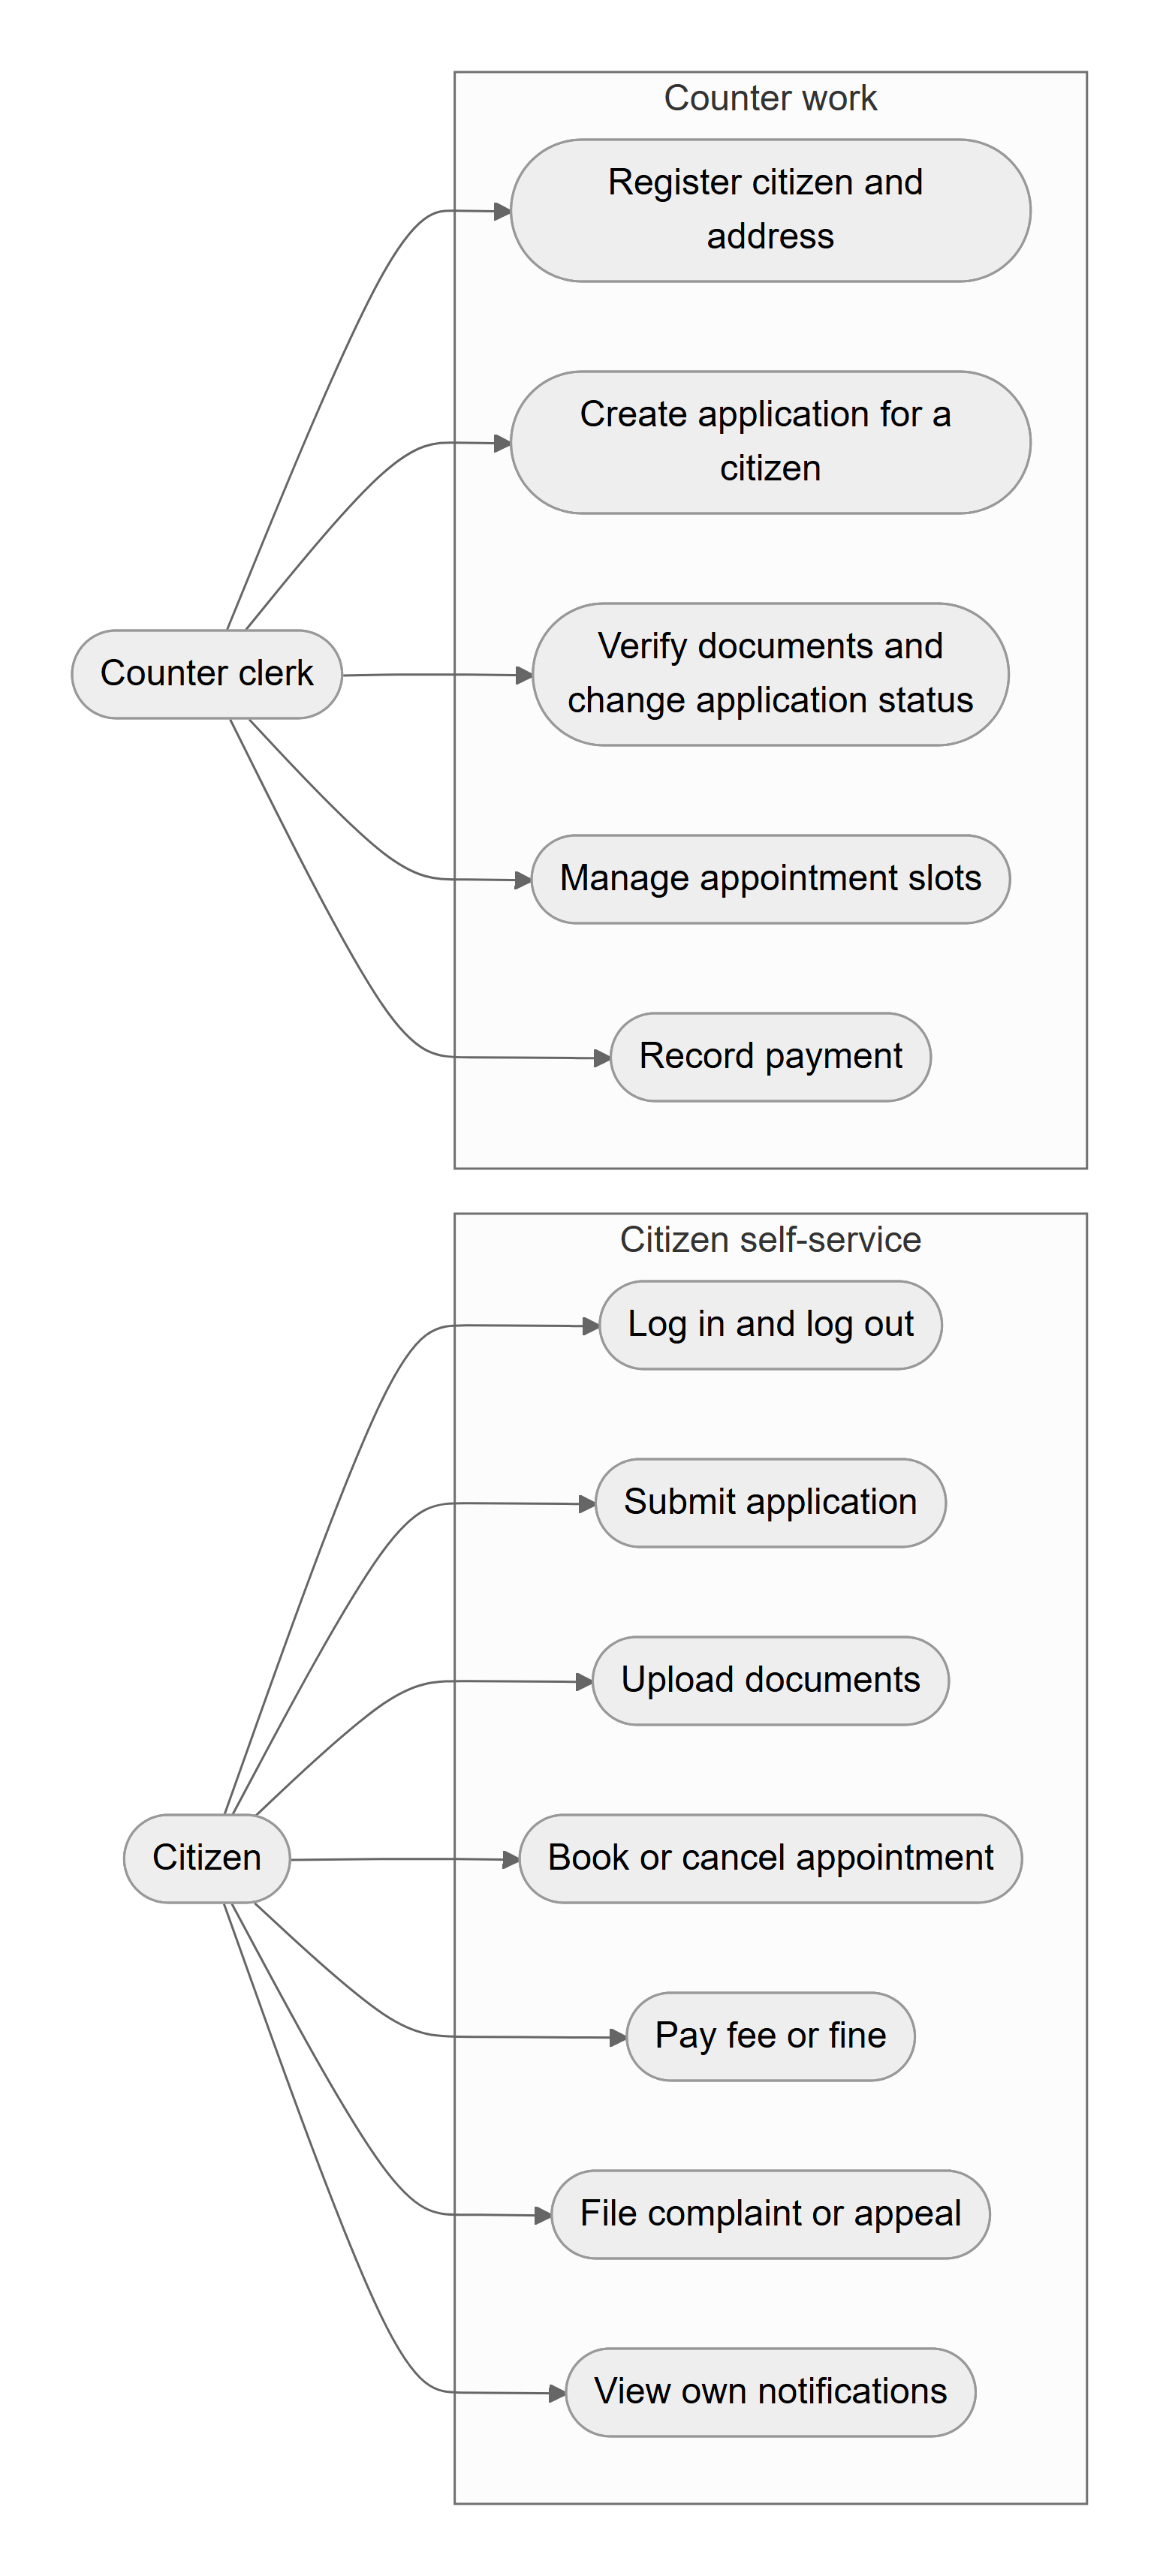
\includegraphics[height=0.42\textheight,keepaspectratio]{usecase_citizen.png}\hfill
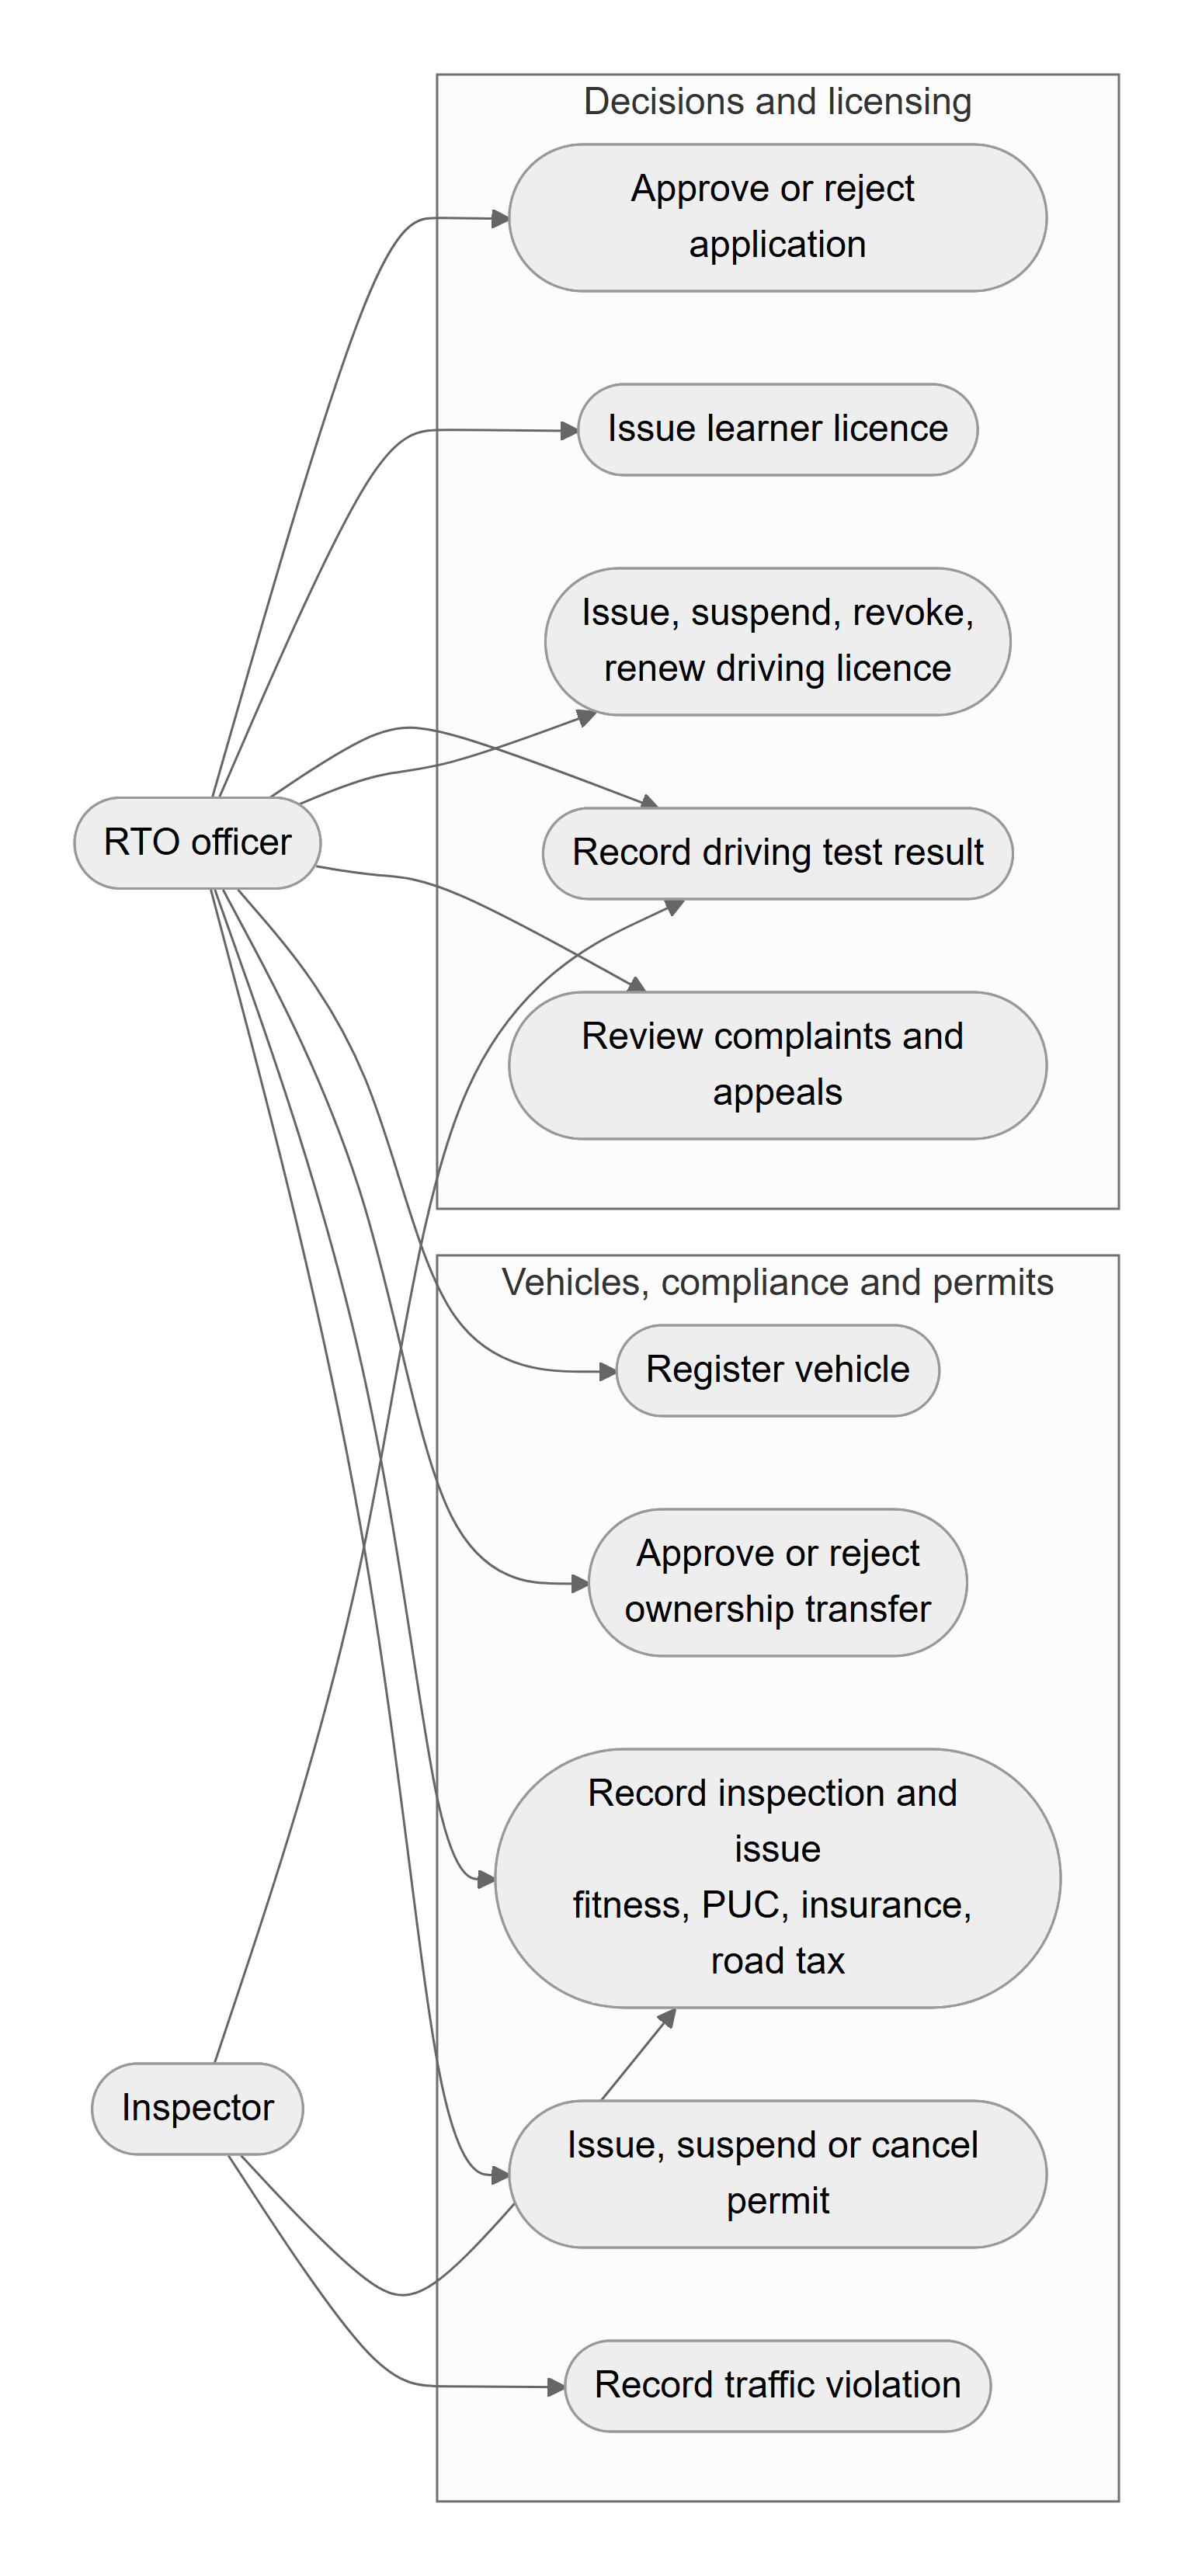
\includegraphics[height=0.42\textheight,keepaspectratio]{usecase_officer.png}
\caption{Use case diagrams: (left) citizen and counter clerk, (right) RTO officer and inspector}\label{fig:uc1}
\end{figure}
\begin{figure}[H]
\centering
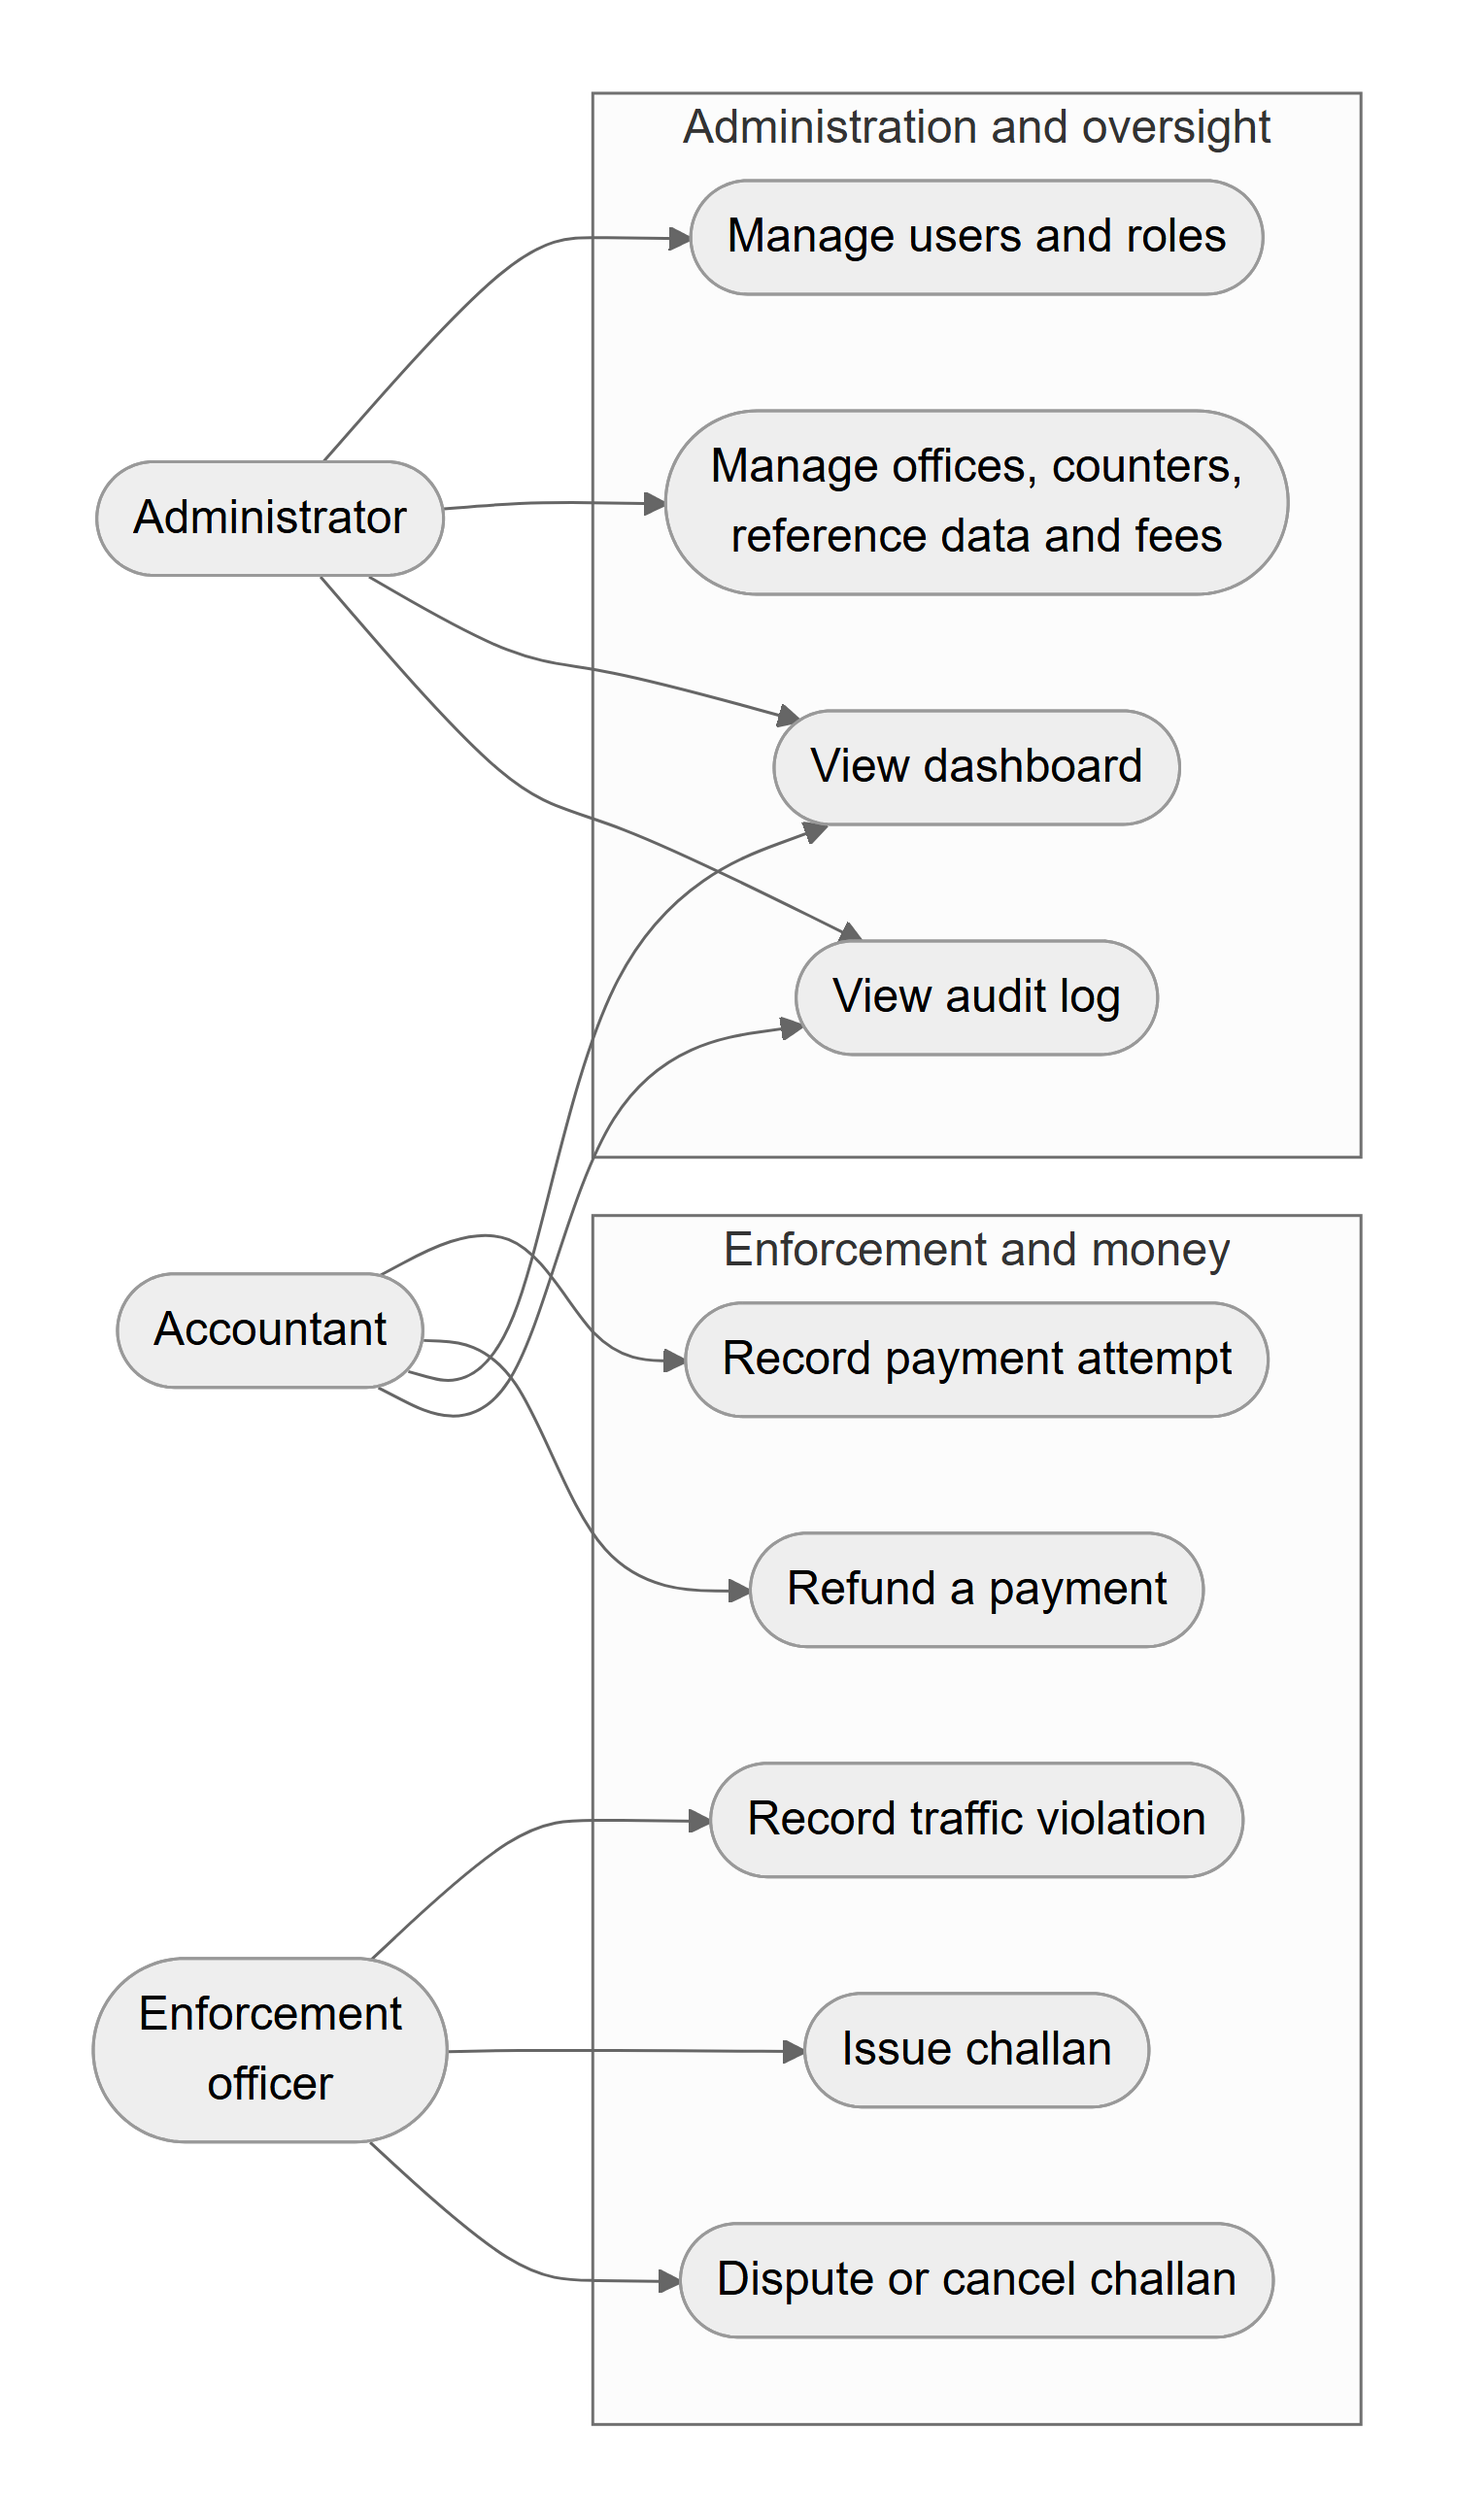
\includegraphics[height=0.40\textheight,keepaspectratio]{usecase_admin.png}
\caption{Use case diagram: enforcement officer, accountant and administrator}\label{fig:uc3}
\end{figure}

\subsection{Class diagram}
Figure~\ref{fig:class} shows the core classes and how they depend on each other. The
important design points are that services depend on \cd{Db}, \cd{Audit} and
\cd{Notifications} but never on each other's data access, and that
\cd{Notifications} depends on the \cd{NotificationProvider} interface, whose mock
implementation can be replaced without changing any caller.

\fig{class_core.png}{Class diagram of the core services and infrastructure}{fig:class}{0.62}

\subsection{Sequence diagrams}
Figure~\ref{fig:seqlogin} shows sign-in and Figure~\ref{fig:seqtransfer} shows approval
of an ownership transfer, the most delicate transaction in the system.

\fig{seq_login.png}{Sequence diagram: sign-in and permission loading}{fig:seqlogin}{0.5}
\fig{seq_transfer.png}{Sequence diagram: approval of an ownership transfer in one transaction}{fig:seqtransfer}{0.4}

\subsection{Activity diagram}
Figure~\ref{fig:activity} follows one service application from creation to completion,
including the loops for missing or rejected documents.

\fig{activity_app.png}{Activity diagram of the application life cycle}{fig:activity}{0.82}

\subsection{State machine diagrams}
Every status field that matters has a transition table in the service code; anything not
in the table is refused with a 409 response. Figure~\ref{fig:stateapp} shows the
application workflow and Figure~\ref{fig:stateother} shows the licence, challan, permit
and vehicle machines.

\fig{state_application.png}{State machine of an application (nine states)}{fig:stateapp}{0.45}
\fig{state_others.png}{State machines of driving licence, challan, permit and vehicle}{fig:stateother}{0.4}

\subsection{Component and deployment diagram}
Figure~\ref{fig:deploy} shows the processes and ports of the development deployment.
Everything runs on one machine; the backend and portal are separate JVM processes.

\fig{deploy.png}{Component and deployment view of the development setup}{fig:deploy}{0.3}

\section{Database Design}
\subsection{Overview}
The schema is created by thirteen scripts, one per module, run in dependency order
(Table~\ref{tab:dbmodules}). The order is not arbitrary: it is a topological order of the
foreign-key graph. We checked this mechanically. Across all 91 foreign keys, no table is
created before a table it references; the longest chain of dependencies has depth six,
and the only self-reference is \cd{regions.parent_region_id}, which lets regions form a
tree.

\begin{table}[H]
\centering\small
\caption{Schema modules, creation scripts and table counts}\label{tab:dbmodules}
\begin{tabularx}{\linewidth}{@{}p{0.9cm}p{3.2cm}cX@{}}
\toprule \textbf{File} & \textbf{Module} & \textbf{Tables} & \textbf{Tables created}\\ \midrule
02 & Reference data & 11 & regions, vehicle\_manufacturers, vehicle\_models, vehicle\_types, fuel\_types, licence\_classes, document\_types, service\_types, violation\_types, permit\_types, payable\_types\\
03 & Identity & 3 & persons, addresses, citizens\\
04 & Office structure & 4 & rto\_offices, departments, designations, counters\\
05 & Employees & 2 & employees, employee\_postings\\
06 & Access control & 5 & users, roles, permissions, user\_roles, role\_permissions\\
07 & Applications & 6 & applicants, applications, application\_status\_history, documents, appointment\_slots, appointments\\
08 & Licensing & 8 & driving\_schools, driving\_instructors, test\_centres, learner\_licences, driving\_licences, licence\_class\_assignments, licence\_status\_history, driving\_tests\\
09 & Vehicles & 3 & vehicles, vehicle\_ownerships, ownership\_transfers\\
10 & Compliance & 5 & vehicle\_inspections, fitness\_certificates, pollution\_certificates, insurance\_policies, road\_tax\_records\\
11 & Permits & 4 & routes, route\_segments, permits, permit\_status\_history\\
12 & Violations & 4 & violations, challans, challan\_violations, challan\_status\_history\\
13 & Payments & 4 & fee\_structures, payments, payment\_attempts, refunds\\
14 & Support & 4 & notifications, complaints, appeals, audit\_logs\\
\midrule
 & \textbf{Total} & \textbf{63} & \\
\bottomrule
\end{tabularx}
\end{table}

\subsection{Entity--relationship diagrams}
The twelve diagrams that follow cover all 63 tables. They were generated from the live
database, so the keys and relationships shown are the real ones. In each diagram
\texttt{PK} marks a primary key, \texttt{FK} a foreign key and \texttt{UK} a unique key.
A solid line with a single bar means the referencing column is mandatory; a line with a
circle means it may be empty. Tables from other modules appear as small boxes with only
their primary key.

\fig{er_org.png}{ER diagram: organisation and staff}{fig:er1}{0.45}
Offices belong to regions (a tree through \cd{parent_region_id}); counters belong to an
office; an employee has a designation and any number of dated postings to an office and a
department. A generated column guarantees that an employee has at most one open posting.

\fig{er_identity.png}{ER diagram: identity and access control}{fig:er2}{0.42}
A \cd{person} is stored once. A citizen and an employee each extend a person, and a user
account is the login for a person. Roles and permissions meet users through the two
junction tables \cd{user_roles} and \cd{role_permissions}, whose primary keys are the pair
of ids.

\fig{er_applications.png}{ER diagram: applications and documents}{fig:er3}{0.5}
An application belongs to an applicant (a citizen's role as a service seeker), a service
type and an office, and may be assigned to an officer. Its status history and its documents
hang from it. The document type supplies the validity period used to decide whether a
verified document has expired.

\fig{er_appointments.png}{ER diagram: appointment slots and bookings}{fig:er4}{0.42}
A slot belongs to an office and optionally a counter and carries a capacity and a booked
count; a CHECK constraint keeps the count within the capacity. An appointment ties one
application to one slot.

\fig{er_licence.png}{ER diagram: learner and driving licences}{fig:er5}{0.5}
A learner licence and a driving licence each reference a citizen and the application that
produced them. A driving licence can carry several classes through
\cd{licence_class_assignments} and keeps its status changes in \cd{licence_status_history}.

\fig{er_tests.png}{ER diagram: driving schools and tests}{fig:er6}{0.36}
Schools have instructors; test centres belong to an office; a driving test links an
application, a citizen, a test centre and an examining employee.

\fig{er_vehicle.png}{ER diagram: vehicles and ownership}{fig:er7}{0.5}
A vehicle references its manufacturer, model, type and fuel and its registering office.
Ownership is a dated history: each row has \cd{effective_from} and \cd{effective_to}, and a
generated column permits only one open row per vehicle. An ownership transfer ties the
old owner, the new owner and the application.

\fig{er_compliance.png}{ER diagram: vehicle compliance records}{fig:er8}{0.5}
Inspections, fitness certificates, pollution certificates, insurance policies and
road-tax records each belong to a vehicle, and several carry date CHECK rules
(expiry after issue).

\fig{er_permits.png}{ER diagram: permits and routes}{fig:er9}{0.4}
Routes have ordered segments; a permit links a vehicle, a permit type and a route, and
its status changes are kept in \cd{permit_status_history}.

\fig{er_enforcement.png}{ER diagram: violations and challans}{fig:er10}{0.4}
A violation belongs to a vehicle and optionally to a driver, who may be unknown. A
challan bundles one or more violations through the junction table
\cd{challan_violations} and keeps its own status history.

\fig{er_payments.png}{ER diagram: fees, payments and refunds}{fig:er11}{0.35}
A payment refers to its target (application, challan, permit or road tax) through a
payable type and an id. It can have many attempts and many refunds.

\fig{er_support.png}{ER diagram: complaints, appeals, notifications and audit}{fig:er12}{0.3}
Complaints and appeals are filed by citizens; notifications are addressed to persons; the
audit log records the table, the record id, the action, the old and new values as JSON,
and the user.

\subsection{Keys and referential integrity}
Every table has a primary key, and 59 of the 63 use an auto-incrementing
\texttt{BIGINT UNSIGNED}. The other four are junction tables whose primary key is the
pair of foreign keys: \cd{user_roles}, \cd{role_permissions},
\cd{licence_class_assignments} and \cd{challan_violations}. There are 91 foreign keys.
The delete rule was chosen per relationship (Table~\ref{tab:fkrules}).

\begin{table}[H]
\centering\small
\caption{Foreign-key delete rules}\label{tab:fkrules}
\begin{tabularx}{\linewidth}{@{}p{2.4cm}cX@{}}
\toprule \textbf{Rule} & \textbf{Count} & \textbf{Used when}\\ \midrule
RESTRICT & 52 & The parent has history that must not be lost: a citizen with licences, a vehicle with owners, an application with payments\\
CASCADE & 29 & Child rows have no meaning without the parent: addresses of a person, counters of an office, segments of a route, junction rows\\
SET NULL & 10 & The link is optional and may be dropped: an assigned officer, a verifying employee, a driver who is unknown\\
\bottomrule
\end{tabularx}
\end{table}

\subsection{Integrity constraints}
The schema uses several kinds of rule.
\begin{itemize}
\item \textbf{43 unique keys} on business identifiers such as national ID, citizen code, registration, chassis and engine numbers, licence numbers, challan numbers and receipt numbers.
\item \textbf{25 ENUM columns} for fixed vocabularies such as status and type, so an invalid status cannot be stored.
\item \textbf{Exact money.} The seven monetary columns are \texttt{DECIMAL(10,2)}; there is no \texttt{FLOAT} or \texttt{DOUBLE} column anywhere in the schema.
\item \textbf{CHECK constraints.} Seven are in the base schema (expiry later than issue for licences, fitness, pollution, insurance and permits; booked seats not above capacity). The constraints script defines 21 more for phone, pincode, positive amounts, slot times and similar rules. MySQL accepts 19 of them and rejects two that use the current date (Section~\ref{sec:defects}), so 26 CHECK constraints are enforced in total.
\item \textbf{Three generated columns} implement ``at most one current row'' (Table~\ref{tab:gen}). Each evaluates to 1 for the current row and to NULL otherwise, and because a unique key ignores NULLs, only one row per entity can be current.
\end{itemize}

\begin{table}[H]
\centering\small
\caption{Generated columns that enforce ``one current row''}\label{tab:gen}
\begin{tabularx}{\linewidth}{@{}p{3.4cm}p{3.0cm}p{3.6cm}X@{}}
\toprule \textbf{Table} & \textbf{Column} & \textbf{Expression} & \textbf{Rule enforced}\\ \midrule
vehicle\_ownerships & current\_flag & \texttt{IF(effective\_to IS NULL, 1, NULL)} & One current owner per vehicle\\
employee\_postings & current\_flag & \texttt{IF(posted\_to IS NULL, 1, NULL)} & One current posting per employee\\
learner\_licences & active\_flag & \texttt{IF(status = 'ACTIVE', 1, NULL)} & One active learner licence per citizen\\
\bottomrule
\end{tabularx}
\end{table}

\subsection{Normalisation}
The schema is designed to third normal form, with a small number of deliberate,
documented exceptions.
\begin{itemize}
\item \textbf{First normal form.} Every column holds one atomic value. A person's addresses are rows in \cd{addresses}, not a list inside \cd{persons}. The only JSON columns are the old and new values in \cd{audit_logs}, which are a log payload, not business data.
\item \textbf{Second normal form.} In the four junction tables the whole key is the pair of ids, and the other columns (for example the date a class was granted) depend on the whole pair.
\item \textbf{Third normal form.} Descriptive attributes live in their own tables: vehicle types, fuel types, licence classes, violation types and service types are lookup tables. The fee and the SLA belong to the service type, not to each application. A citizen's name, phone and e-mail belong to the person, not repeated in the citizen, employee and user tables.
\end{itemize}
\textbf{Deliberate exceptions.}
(a) A vehicle stores both a manufacturer and a model although a model already belongs to
a manufacturer. Keeping both allows filtering by manufacturer without a join, and the
service rejects a pair that does not match (the error \cd{MODEL_MANUFACTURER_MISMATCH}).
(b) The current status of an application, licence, permit and challan is stored on the
row as well as in the history table, so the present state is a single read while the whole
history is still available.
(c) A challan stores \cd{total_amount}, which is derivable from its violations. It is kept
as an exact decimal and recalculated by the service when violations are added or removed.

\subsection{Indexing strategy}
InnoDB creates an index for every primary key, unique key and foreign key, so the
schema starts with 192 index entries. The script \cd{16_indexes.sql} adds 25 more, each
justified by a real query pattern found in the service layer (Table~\ref{tab:indexes}).
Chapter~\ref{ch:perf} measures the effect of two of them.

\begingroup\footnotesize
\begin{longtable}{@{}p{4.6cm}p{4.6cm}p{5.4cm}@{}}
\caption{The 25 added indexes and the queries they serve}\label{tab:indexes}\\
\toprule \textbf{Index} & \textbf{Table (columns)} & \textbf{Query served}\\ \midrule \endfirsthead
\toprule \textbf{Index} & \textbf{Table (columns)} & \textbf{Query served}\\ \midrule \endhead
\bottomrule \endlastfoot
idx\_application\_submitted\_date & applications (submitted\_at) & Date-range listing\\
idx\_application\_assigned\_officer & applications (assigned\_officer\_id, current\_status) & Officer workload\\
idx\_application\_service\_type & applications (service\_type\_id) & Listing and fee lookup\\
idx\_citizen\_blacklisted & citizens (blacklisted) & Blacklist filter\\
idx\_person\_email & persons (email) & E-mail resolution\\
idx\_user\_active\_login & users (username, is\_active) & Login lookup\\
idx\_user\_last\_login & users (last\_login\_at) & Security dashboards\\
idx\_violation\_occurred & violations (occurred\_at) & Date-range reports\\
idx\_violation\_officer & violations (officer\_employee\_id) & Officer workload\\
idx\_challan\_issued\_at & challans (issued\_at) & Date-range reports\\
idx\_payment\_created\_at & payments (created\_at) & Financial reports\\
idx\_payment\_paid\_at & payments (paid\_at) & Reconciliation\\
idx\_attempt\_gateway\_ref & payment\_attempts (gateway\_reference) & Idempotency lookup on every payment\\
idx\_dl\_expiry & driving\_licences (expiry\_date, current\_status) & Renewal dashboard\\
idx\_ll\_expiry & learner\_licences (expiry\_date, status) & Conversion deadlines\\
idx\_permit\_expiry\_status & permits (expiry\_date, status) & Permit compliance\\
idx\_fitness\_expiry\_status & fitness\_certificates (expiry\_date, status) & Expiry batch jobs\\
idx\_puc\_expiry\_status & pollution\_certificates (expiry\_date, status) & Expiry batch jobs\\
idx\_insurance\_end\_date & insurance\_policies (end\_date) & Renewal alerts\\
idx\_road\_tax\_status\_due & road\_tax\_records (status, due\_date) & Overdue sweep\\
idx\_notification\_person\_status & notifications (person\_id, status) & Delivery queue\\
idx\_notification\_sent\_at & notifications (sent\_at) & History reports\\
idx\_complaint\_office\_status & complaints (office\_id, status) & Staff workload\\
idx\_appeal\_status & appeals (status, filed\_at) & Review queue\\
idx\_posting\_office\_current & employee\_postings (office\_id, posted\_to) & Who is posted at an office\\
\end{longtable}
\endgroup

\subsection{Views}
Six read-only views hide long joins from reports and administrators. The backend does not
map them to entities.
\begin{table}[H]
\centering\small
\caption{Database views}\label{tab:views}
\begin{tabularx}{\linewidth}{@{}p{5.0cm}X@{}}
\toprule \textbf{View} & \textbf{Purpose}\\ \midrule
vw\_current\_vehicle\_owners & Each vehicle with its current owner and registering office\\
vw\_pending\_applications & Applications not yet finished, with an SLA-breach flag and days elapsed\\
vw\_outstanding\_challans & Issued challans with violation, vehicle and officer details\\
vw\_expiring\_compliances & Pollution, fitness and insurance records expiring within 30 days\\
vw\_active\_driving\_licences & Active licences with the classes held, as a comma-separated list\\
vw\_application\_status\_summary & Counts and average age of applications per office and status\\
\bottomrule
\end{tabularx}
\end{table}

\subsection{Triggers and stored procedures}\label{sec:trigdesign}
\textbf{Where a trigger belongs.} The trigger script begins with an analysis of what
the Java services already write. Application and challan history and the audit log are
written by the services, so triggers for them would create duplicate rows. Triggers were
therefore added only for rules the backend does not already own, or that must hold for any
SQL client (Table~\ref{tab:triggers}).

\begin{table}[H]
\centering\small
\caption{Triggers}\label{tab:triggers}
\begin{tabularx}{\linewidth}{@{}p{4.9cm}p{3.1cm}X@{}}
\toprule \textbf{Trigger} & \textbf{Fires} & \textbf{Effect}\\ \midrule
trg\_after\_licence\_status\_change & AFTER UPDATE on driving\_licences & Appends a licence\_status\_history row when the status changes\\
trg\_after\_permit\_status\_change & AFTER UPDATE on permits & Appends a permit\_status\_history row when the status changes\\
trg\_before\_vehicle\_delete & BEFORE DELETE on vehicles & Refuses deletion of an ACTIVE vehicle\\
trg\_before\_licence\_delete & BEFORE DELETE on driving\_licences & Refuses deletion of an ACTIVE licence\\
trg\_before\_road\_tax\_update & BEFORE UPDATE on road\_tax\_records & Turns DUE into OVERDUE when the due date has passed\\
\bottomrule
\end{tabularx}
\end{table}

\textbf{Stored procedures.} Three procedures package multi-step operations for
administrators and batch jobs (Table~\ref{tab:procs}). The backend does not call them; it
performs the same operations in its own transactions.

\begin{table}[H]
\centering\small
\caption{Stored procedures}\label{tab:procs}
\begin{tabularx}{\linewidth}{@{}p{5.0cm}X@{}}
\toprule \textbf{Procedure} & \textbf{What it does}\\ \midrule
sp\_transfer\_vehicle\_ownership & Locks the transfer, vehicle and current ownership; checks the status, owner and dates; closes the old ownership, opens the new one and marks the transfer approved; rolls everything back on any error\\
sp\_process\_challan\_payment & Locks the challan, refuses a gateway reference that was already used, creates the payment and its attempt, marks the challan paid and appends the history, in one transaction\\
sp\_update\_overdue\_road\_tax & Marks every DUE road-tax record whose due date has passed as OVERDUE and returns how many were changed\\
\bottomrule
\end{tabularx}
\end{table}

\subsection{Sample records}
Table~\ref{tab:sample} shows a few rows returned by the ``vehicles without current
insurance'' query of the advanced-query script, run against the small seed dataset.
\begin{table}[H]
\centering\footnotesize
\caption{Sample output: vehicles and their insurance status (query Q2, seed 22, run on 3 November 2026)}\label{tab:sample}
\begin{tabularx}{\linewidth}{@{}p{2.2cm}p{2.0cm}p{2.7cm}p{2.0cm}p{2.1cm}X@{}}
\toprule \textbf{Registration} & \textbf{Status} & \textbf{Make and model} & \textbf{Insurance} & \textbf{Ends on} & \textbf{Provider}\\ \midrule
GJ01AB1234 & ACTIVE & Maruti Suzuki Swift & EXPIRED & 2026-10-25 & New India Assurance\\
GJ01CD5678 & ACTIVE & Hero Splendor Plus & EXPIRED & 2026-07-20 & Bajaj Allianz\\
GJ21EF9012 & ACTIVE & Tata Nexon & INSURED & 2027-01-01 & HDFC Ergo\\
GJ21GH3456 & ACTIVE & Mahindra Bolero & UNINSURED & -- & --\\
\bottomrule
\end{tabularx}
\end{table}

\section{Security and Error-Handling Design}\label{sec:security}
\subsection{Authentication}
A user signs in with a username and password. The backend looks the user up and verifies
the password against a BCrypt hash (cost factor 12). When the username does not exist,
it verifies the password against a dummy hash instead, so that the response time does not
tell an attacker which usernames are valid. A wrong password and an unknown user return the
same message. On success the backend returns an access token (30 minutes by default) and a
refresh token (7 days). Both are HS256 JSON Web Tokens \cite{rfc7519} with a unique id.

Token handling has three extra safeguards. A token must have exactly three base64url parts
that re-encode to the same text, which rejects tokens with junk appended to the signature
that lenient decoders would silently accept. The token type is checked, so a refresh token
cannot be used as an access token. And refresh tokens rotate: using one revokes it and
issues a new pair. Revoked token ids are held in memory until they expire.

\subsection{Authorisation}
Each endpoint is annotated with \cd{@Public}, \cd{@Requires("permission")} or
\cd{@RequiresAny}. A single interceptor reads the annotation and decides \emph{before} the
controller runs. The permissions of the user are loaded on every request from
\cd{user_roles}, \cd{role_permissions} and \cd{permissions}; nothing is cached or
hard-coded per user. Consequently, when an administrator changes a role, the next request
of every holder sees the change, and a deactivated user loses access even with a token that
has not expired (both are covered by tests).

For record-level rules the service applies a second check. Permissions that end in
\cd{_own} restrict a citizen to records linked to their own person or citizen id, and the
national ID number is hidden from lists and from users who lack
\cd{citizen.view_sensitive}. Figure~\ref{fig:perm} shows the decision procedure.

\fig{flow_perm.png}{Permission decision in the authentication interceptor}{fig:perm}{0.7}

\subsection{Input validation and injection}
Request bodies are Java records with Bean Validation annotations (patterns for phone,
national ID and e-mail; length limits; required fields), and a failure returns 422 with a
list of field and message pairs. Passwords must have at least 8 characters and at most 72
bytes (the BCrypt limit). All queries go through JPA or parameterised JPQL; no SQL string
is built from user input, which removes the usual route for SQL injection.

\subsection{File uploads}
A document upload is accepted only if the extension is \texttt{pdf}, \texttt{png},
\texttt{jpg} or \texttt{jpeg}, the first bytes of the file match that type (for example
\texttt{\%PDF}), the file is not empty and it is within the size limit (10~MB by
default). The file is stored on disk and only its path goes in the database. Documents
cannot be added to an application in a terminal state.

\subsection{Errors and consistency}
All backend errors share one JSON shape with the fields \texttt{detail}, \texttt{code} and an optional list \texttt{errors}. A mapper turns
database errors into the same shape: a duplicate key (MySQL error 1062) becomes a 409 with
a readable message, a CHECK violation becomes a 409, a missing parent row becomes a 400,
and a deadlock or lock timeout becomes a ``please retry'' conflict. No SQL text or stack
trace is returned to the client. Because each service method is one transaction, any
exception rolls back every change made in that call.

The portal adds its own layer. \cd{GlobalAdvice} turns API and system errors into
pages with the right status: 403 and 404 pages in plain language, a 405 page for an
address that accepts only a form post, and a generic 500 page that logs the details on the
server and shows none. A 401 sends the user back to sign in. Form errors from the API are
mapped to the individual fields.

\begin{table}[H]
\centering\small
\caption{Error handling by situation}\label{tab:errors}
\begin{tabularx}{\linewidth}{@{}p{3.6cm}p{2.0cm}X@{}}
\toprule \textbf{Situation} & \textbf{Status} & \textbf{Behaviour}\\ \midrule
No or invalid token & 401 & Backend returns the error; portal redirects to sign-in\\
Missing permission & 403 & Plain-language page; nothing is changed\\
Record not found & 404 & ``The record you asked for was not found''\\
Invalid input & 422 / 400 & Field-level messages; the form is shown again with the entered values\\
Illegal status move, duplicate, full slot & 409 & Clear conflict message; nothing is changed\\
Competing update (deadlock, lock timeout) & 409 & ``Please retry''\\
Backend not running & 503 & Page explaining that the backend cannot be reached\\
Unexpected failure & 500 & Details logged on the server; generic message shown\\
\bottomrule
\end{tabularx}
\end{table}

\subsection{Audit and privacy}
Every service that changes important data writes a row to \cd{audit_logs} in the
\emph{same} transaction as the change, so an audit entry exists if and only if the change
committed. There is no update or delete operation for the audit log. Before a row is
written, any key whose name contains \texttt{password}, \texttt{secret},
\texttt{access\_token}, \texttt{refresh\_token} or \texttt{national\_id\_number} is dropped,
so secrets never reach the log; a test checks this.

\chapter{Algorithm Design and Data Structures}\label{ch:algo}

\section{Identification of Critical Operations}
Most of the system is straightforward reading and writing of rows. A few operations,
however, decide whether the system is \emph{correct}, and they are where algorithm design
matters. Table~\ref{tab:critical} lists them.

\begin{table}[H]
\centering\small
\caption{Critical operations and what makes them critical}\label{tab:critical}
\begin{tabularx}{\linewidth}{@{}p{0.9cm}p{4.2cm}X@{}}
\toprule \textbf{ID} & \textbf{Operation} & \textbf{Why it is critical}\\ \midrule
A1 & Resolve and check permissions on every request & Security decision made hundreds of times per minute; must be cheap and always current\\
A2 & Book an appointment slot & Two users may compete for the last seat; overbooking is a visible failure\\
A3 & Approve an ownership transfer & A vehicle must have exactly one current owner before and after\\
A4 & Record a payment attempt & A retried request must not charge twice or lose a failed attempt\\
A5 & Validate a status transition & Wrong moves (for example reopening a completed application) corrupt history\\
A6 & Build a filtered, sorted, paged list & Used by every list screen; must be safe against injection and bounded in size\\
A7 & Prevent a cycle in the region hierarchy & A region that is its own ancestor would break tree traversal\\
A8 & Order the creation of 63 tables & A table cannot be created before the tables it references\\
\bottomrule
\end{tabularx}
\end{table}

\section{Algorithm Design}
The algorithms are given in pseudocode that follows the structure of the implementation.
Lines that start with \textsf{LOCK} correspond to \cmd{SELECT ... FOR UPDATE}.

\subsection{A1: permission resolution and check}
\begin{lstlisting}[language={},mathescape=false]
resolveUser(userId):
    user  <- select user by id; if none or inactive: 401
    roles <- select role names via user_roles
    perms <- SET of distinct permission keys via
             user_roles JOIN role_permissions JOIN permissions
    emp   <- active employee of user's person (if any)
    return CurrentUser(user, roles, perms, emp, ...)

check(handler, user):
    if handler is @Public: allow
    if user is none: 401
    for key in @Requires(handler): if key not in user.perms: 403
    if @RequiresAny(handler) and none of its keys in user.perms: 403
    allow
\end{lstlisting}
The permission set is a hash set, so each membership test is $O(1)$. Loading it costs a
few indexed joins per request; because it is read each time, a change to a role takes
effect immediately.

\subsection{A2: booking a slot}
\begin{lstlisting}[language={},mathescape=false]
book(application, slot):
    LOCK application
    LOCK slots in ascending id order        // TreeSet of ids
    require slot.office == application.office
    require slot start is in the future
    n <- UPDATE slot SET booked = booked + 1
         WHERE id = slot AND booked < capacity   // guarded update
    if n == 0: 409 SLOT_FULL
    token <- "S{slot}-{ (highest suffix among slot tokens) + 1 }"
    insert appointment(BOOKED, token); insert audit row
    queue notification (delivered after commit)
\end{lstlisting}
Three layers prevent overbooking. The lock serialises competing bookers; the guarded
\cmd{UPDATE ... WHERE booked_count < capacity} is an atomic compare-and-set that refuses
to increment past the capacity even if the lock were somehow missed; and the table's
CHECK constraint (\cd{booked_count <= capacity}) is the last line of defence. The token
is computed while the slot is locked, so two callers can never receive the same number.
Figure~\ref{fig:flowbook} shows the flow.

\fig{flow_booking.png}{Flowchart of slot booking}{fig:flowbook}{0.72}

\subsection{A3: approving an ownership transfer}
\begin{lstlisting}[language={},mathescape=false]
approve(transferId, date):
    LOCK transfer;  require status == PENDING
    LOCK vehicle;   require status == ACTIVE
    LOCK current ownership row (effective_to IS NULL)
    require ownership.citizen == transfer.from_citizen
    require transferee not blacklisted
    require ownership.effective_from <= date <= today
    ownership.effective_to <- date       // close the old row
    FLUSH                                 // old row must reach the DB first
    insert ownership(vehicle, to_citizen, effective_from = date)
    transfer.status <- APPROVED; transfer.approved_at <- now
    insert audit rows; queue notifications
    COMMIT   (any failure above: ROLLBACK everything)
\end{lstlisting}
The explicit flush matters. The unique key on the generated column
\cd{vehicle_ownerships.current_flag} allows one open row per vehicle, so the old row must be
closed in the database \emph{before} the new open row is inserted; otherwise the insert would
violate the key. A dedicated test (\texttt{aFailureMidApprovalRollsEverythingBack}) forces
a failure after the first changes and checks that nothing remains. Figure~\ref{fig:flowtransfer}
shows the flow.

\fig{flow_transfer.png}{Flowchart of ownership-transfer approval}{fig:flowtransfer}{0.75}

\subsection{A4: idempotent payment}
\begin{lstlisting}[language={},mathescape=false]
payTarget(type, id, reference, outcome):
    prior <- attempt with this gateway reference          // indexed lookup
    if prior exists:
        if prior.payment is for the same (type, id): return it   // replay
        else: 409 GATEWAY_REFERENCE_REUSED
    LOCK target;  if a SUCCESS payment exists: 409 ALREADY_PAID
    payment <- reuse open PENDING/FAILED payment or create one
               (amount = amount due, never taken on trust)
    LOCK payment
    insert attempt(number = max + 1, reference, outcome)
    SUCCESS -> payment SUCCESS, settle target (challan PAID ...)
    FAILED  -> payment FAILED (retry allowed)
    TIMEOUT -> payment stays PENDING (result unknown)
\end{lstlisting}
The gateway reference acts as an \emph{idempotency key}: the same reference always yields
the same result, and the replay is answered \emph{before} the target is validated, because
the item may legitimately be paid by now. The \cd{idx_attempt_gateway_ref} index keeps this
lookup fast (Chapter~\ref{ch:perf}). A timeout deliberately does not mark the payment failed:
the gateway outcome is unknown, so the payment stays pending and can be reconciled.
Figure~\ref{fig:flowpay} shows the flow.

\fig{flow_payment.png}{Flowchart of an idempotent payment}{fig:flowpay}{0.75}

\subsection{A5: status transition validation}
Each workflow has a table of legal moves, a map from a status to the set of statuses
that may follow it. A move is accepted only if the target is in the set of the current
status, and some targets additionally require a permission and a reason.
\begin{lstlisting}[language={},mathescape=false]
TRANSITIONS = { SUBMITTED: {DOCS_PENDING, UNDER_VERIFICATION, REJECTED, CANCELLED},
                ... , APPROVED: {COMPLETED}, REJECTED: {}, COMPLETED: {}, CANCELLED: {} }

applyStatus(app, next, reason):
    if next not in TRANSITIONS[app.status]: 409 INVALID_TRANSITION
    if next in {REJECTED, CANCELLED, DOCS_PENDING} and reason is empty: reject (validation error)
    require permission PERMISSION_FOR_TARGET[next]
    append history row(prev, next, user, reason); app.status <- next
\end{lstlisting}

\subsection{A6: filtered, sorted, paged lists}
A small query builder appends a condition only when its value is present, binds every value
as a parameter, escapes the characters \texttt{\%} and \texttt{\_} in search text, and
accepts a sort key only if it is in a whitelist. A list request runs a \texttt{COUNT} over
the filtered query and then one bounded page (at most 100 rows), and returns the items with
the page number, page size, total and page count.

\subsection{A7: region hierarchy}
Regions form a tree through \cd{parent_region_id}. Before a parent is assigned, the
service walks up the parent chain from the proposed parent; if it meets the region
itself, the change is refused with \cd{REGION_CYCLE}. The region tree for display is built in
one pass: every region becomes a node in a hash map by id, and each node with a parent is
appended to its parent's list of children.

\subsection{A8: dependency-ordered schema creation}
Treat the 63 tables as vertices and each foreign key as a directed edge from the
referencing table to the referenced table. A table can be created only after all the tables
it points to, so a valid creation order is a topological order of this directed acyclic
graph. We computed the longest-path level of every table and checked that the order used
by the scripts respects every edge. There are $V=63$ vertices and $E=90$ edges once the
single self-reference (\cd{regions}) is set aside, and the levels run from 0 to 6
(Table~\ref{tab:levels}). Topological ordering and level computation take $O(V+E)$ time,
which here is 153 elementary steps; the check found no edge pointing backwards.

\begin{table}[H]
\centering\small
\caption{Dependency depth of the 63 tables}\label{tab:levels}
\begin{tabularx}{\linewidth}{@{}cp{1.6cm}X@{}}
\toprule \textbf{Level} & \textbf{Tables} & \textbf{Examples}\\ \midrule
0 & 18 & document\_types, fuel\_types, departments, designations, challans, audit\_logs\\
1 & 12 & citizens, employees, addresses, fee\_structures, notifications\\
2 & 11 & applicants, appeals, complaints, counters, driving\_schools, employee\_postings\\
3 & 9 & applications, appointment\_slots, driving\_instructors, insurance\_policies\\
4 & 9 & documents, appointments, driving\_tests, fitness\_certificates, challan\_violations\\
5 & 2 & driving\_licences, permit\_status\_history\\
6 & 2 & licence\_class\_assignments, licence\_status\_history\\
\bottomrule
\end{tabularx}
\end{table}

\section{Flowcharts}
The flowcharts of the three transactional algorithms are Figures~\ref{fig:flowbook},
\ref{fig:flowtransfer} and~\ref{fig:flowpay}; the permission decision is
Figure~\ref{fig:perm}; the request life cycle is Figure~\ref{fig:request}.

\section{Data Structure Selection}
Table~\ref{tab:ds} lists the data structures that matter and why each was chosen.

\begin{table}[H]
\centering\small
\caption{Data structures and where they are used}\label{tab:ds}
\begin{tabularx}{\linewidth}{@{}p{3.1cm}p{4.3cm}X@{}}
\toprule \textbf{Structure} & \textbf{Used for} & \textbf{Reason}\\ \midrule
Hash map of sets & Status transition tables for applications, licences, permits, vehicles, challans, complaints and appeals & Constant-time lookup of the allowed next states\\
Hash set & A user's permission keys; redacted audit keys; allowed file extensions & Constant-time membership tests\\
Sorted set (tree set) & Slot ids to lock, so that locks are always taken in ascending order & Gives a canonical order and removes duplicates in $O(s\log s)$\\
Concurrent hash map & Revoked token ids with their expiry times & Safe for many threads; expired entries are purged when a new one is added\\
Insertion-ordered map & Audit values and JSON bodies & Keeps field order stable in the log\\
Tree (adjacency by parent id) & Region hierarchy & Natural for ``belongs to'' with unlimited depth\\
Directed acyclic graph & Foreign-key dependencies & Defines a valid table creation order\\
B$^+$-tree index (InnoDB) & Every primary, unique and secondary key & $O(\log n)$ point and range lookups\\
Table used as a queue & Notifications: QUEUED then SENT or FAILED & Durable before delivery is attempted; survives a restart\\
List & Result pages, sorted permission lists, collected rows & Simple ordered collections\\
\bottomrule
\end{tabularx}
\end{table}

\section{Algorithm Selection and Justification}
\paragraph{Pessimistic locking over optimistic versioning.} The contested rows (the last
seat of a slot, the single current owner, the payment of one challan) are exactly the
rows where conflicts are likely. Optimistic locking would let both writers do the work
and make one of them retry, which is wasteful for hot rows. A short row lock is cheaper
and keeps the code simple. The cost is that competing writers wait, which is acceptable
for office-scale traffic.

\paragraph{Ordered locking against deadlock.} A deadlock needs a cycle in the
``waits-for'' relation between transactions. If every transaction acquires locks of the
same kind in a single global order, such a cycle is impossible, because a transaction
waiting for a lock of higher rank can never be waited for by the holder of that lock
unless it also held a lock of higher rank. The implementation fixes the order inside each
operation family: application, then appointment, then slots in ascending id; transfer,
then vehicle, then ownership row; target, then payment. When two slots are involved, as in
a reschedule, the ids are sorted first. The database can still detect a rare deadlock and
abort one victim; the error mapper turns that into a ``please retry'' response.

\paragraph{Guarded update over read-modify-write.} Reading \texttt{booked\_count},
adding one in Java and writing it back is a race. Putting the condition in the
\texttt{WHERE} clause makes the check and the change a single atomic statement.

\paragraph{Idempotency key over de-duplication by time.} Rejecting a ``similar payment a few
seconds ago'' would be a guess. A unique reference supplied by the caller gives an exact
rule.

\paragraph{Offset paging.} Lists use \texttt{LIMIT}/\texttt{OFFSET} because office lists are
short and users jump to arbitrary pages. For very large tables, key-set paging would be
faster; this is discussed in Section~\ref{sec:opt}.

\section{Time Complexity Analysis}
Let $n$ be the number of rows in a table, $k$ the number of rows matched by a query, $p$
the page size, $s$ the number of slots locked together, $b$ the number of bookings in one
slot and $d$ the depth of the region tree.

\begin{table}[H]
\centering\small
\caption{Time complexity of the critical operations}\label{tab:time}
\begin{tabularx}{\linewidth}{@{}p{4.3cm}p{2.9cm}X@{}}
\toprule \textbf{Operation} & \textbf{Cost} & \textbf{Explanation}\\ \midrule
Permission membership test & $O(1)$ expected & Hash set lookup\\
Load a user's permissions & $O(\log n + k)$ per query & Indexed joins over the user's role and permission rows\\
Status transition check & $O(1)$ expected & Map lookup, then set membership\\
Lock one row by key & $O(\log n)$ & Primary-key index descent\\
Slot booking & $O(s\log s + s\log n + b)$ & Sort ids, lock $s$ rows, guarded update, scan the slot's $b$ tokens for the next number\\
Ownership approval & $O(\log n)$ & A constant number of indexed lookups and writes\\
Payment replay lookup & $O(\log n)$ with the index; $O(n)$ without & Lookup by gateway reference\\
Paged list & $O(\log n + p)$ to return a page; offset adds $O(\text{offset})$ & Count plus bounded page\\
Region cycle check & $O(d)$ queries & Walk up the chain\\
Region tree build & $O(n)$ & One pass with a hash map\\
Schema ordering and check & $O(V+E)$ & Topological order of the foreign-key graph\\
\bottomrule
\end{tabularx}
\end{table}
The difference between $O(n)$ and $O(\log n)$ for the payment lookup is not only
theoretical: on 500\,000 rows, the lookup took 405.9~ms as a full scan and 1.4~ms through
the index (Section~\ref{sec:indexres}).

\section{Space Complexity Analysis}
The algorithms need little extra memory. A permission set holds at most 62 strings per
request. Locking $s$ slots keeps $s$ entities in memory, $O(s)$. A page holds at most $p\le
100$ rows. The region tree holds $O(n)$ nodes for $n$ regions. The revoked-token map holds one
entry per revoked token until its expiry, so its size is proportional to the number of
sign-outs and refreshes within one token lifetime. The topological check needs $O(V+E)$
space for the adjacency data. Persistent storage grows with the number of records and is
governed by the database.

\section{Optimization Opportunities}\label{sec:opt}
\begin{itemize}
\item \textbf{Key-set paging.} For tables with millions of rows, replace the offset by a ``rows after this key'' condition so that deep pages cost $O(\log n + p)$.
\item \textbf{Cache permissions briefly.} A per-user cache with a short lifetime would remove the two permission queries per request, at the price of a small delay before a role change takes effect; we chose freshness over speed.
\item \textbf{Token sequence per slot.} The next token number is found by scanning the slot's tokens; a counter column on the slot would make it $O(1)$.
\item \textbf{Shared revocation store.} Replace the in-memory revoked-token map by a shared store before running several backend instances.
\item \textbf{Batch notification delivery.} Deliver queued messages in batches by a scheduled job instead of one transaction per message when volume grows.
\item \textbf{Measure first.} Each of these should be justified by a measurement; the performance chapter shows where the time actually goes.
\end{itemize}

\chapter{Subject-Wise Engineering Concepts}\label{ch:subjects}
This project was meant to bring five courses of the programme to bear on a single
system. This chapter shows, course by course, which concepts were used, where in the
project they appear and what evidence there is. Concepts are listed only where we can point
to the code, the schema or a test; a course topic that the project does not use is not
claimed.

\section{CE102: Problem Solving using Object Oriented Programming (Lab)}\label{sec:oop}
The backend and the portal are Java 21 programs of about 16\,000 lines (backend 11\,300, portal
4\,900), written around the object-oriented ideas of the lab course.

\begin{table}[H]
\centering\small
\caption{Object-oriented concepts in the project}\label{tab:oop}
\begin{tabularx}{\linewidth}{@{}p{3.3cm}p{5.2cm}X@{}}
\toprule \textbf{Concept} & \textbf{Where it appears} & \textbf{Why it matters here}\\ \midrule
Encapsulation & Each service hides its queries and rules behind public methods; entities have private fields with accessors; controllers never touch the database & Rules live in one place, so a rule is changed once\\
Abstraction and interfaces & \cd{NotificationProvider} interface with the implementation \cd{MockNotificationProvider} & A real SMS or e-mail provider can replace the mock without changing any caller\\
Inheritance and polymorphism & \cd{ReferenceControllers.Base<E, C>} is an abstract base class with ten subclasses for the reference resources; \cd{ApiException} extends \cd{RuntimeException} & One class provides list, get, create, update and delete for ten resources\\
Generics & \cd{Base<E, C>}, \cd{PageResponse<T>}, \cd{Db.list(Class<T>, ...)}, \cd{Db.page(...)} & Type-safe reuse without casting\\
Records & Request and response DTOs, \cd{PageParams}, \cd{PageResponse} & Immutable data carriers with built-in equality and accessors\\
Custom annotations and reflection & \cd{@Public}, \cd{@Requires}, \cd{@RequiresAny}, \cd{@ValidPassword}; \cd{AuthInterceptor} reads them at run time & Access rules are declared next to the code they protect\\
Exceptions & \cd{ApiException} with status and code; \cd{GlobalExceptionHandler}; database error translation & A runtime exception rolls the transaction back; the client gets a uniform error\\
Collections, streams, lambdas & Maps of sets for transitions; streams for filtering and mapping; lambdas in the after-commit hook & Compact, readable data handling\\
Value types & \cd{BigDecimal} for all money; \cd{java.time} for dates and times & No rounding error; clear handling of time zones (UTC)\\
Dependency injection & Constructor injection of services into services and controllers & Loose coupling and easy replacement in tests\\
Design patterns & Strategy (notification provider); Template Method (reference base class); Fluent builder (\cd{QB}); Chain of responsibility (JWT filter, then interceptor, then controller); Utility class with a private constructor (\cd{Perms}, \cd{Fees}) & Familiar structures that make the code easier to read\\
Concurrency & \cd{ConcurrentHashMap} for revoked tokens; transactions and row locks; tests that start threads together using a \cd{CountDownLatch} & Safe behaviour with many simultaneous users\\
\bottomrule
\end{tabularx}
\end{table}
\textbf{A design choice, stated plainly.} Statuses such as \texttt{ACTIVE} or
\texttt{APPROVED} are Java strings in the code and \texttt{ENUM} columns in the database,
not Java enums. This keeps the code close to the schema, and the transition tables catch
wrong values, but Java enums would add compile-time safety. We note this as a possible
improvement.

\section{CE204: Database Management}\label{sec:dbms}
This is the course the project leans on most.

\begin{table}[H]
\centering\small
\caption{Database concepts in the project}\label{tab:dbms}
\begin{tabularx}{\linewidth}{@{}p{3.4cm}p{6.1cm}X@{}}
\toprule \textbf{Concept} & \textbf{How it is used} & \textbf{Evidence}\\ \midrule
ER modelling & 12 ER diagrams covering 63 tables, generated from the live schema & Section 4.6\\
Relational schema and keys & 59 surrogate keys, 4 composite keys, 43 unique keys, 91 foreign keys & Schema dump\\
Generalisation & \cd{persons} is the parent; \cd{citizens} and \cd{employees} extend it; \cd{applicants} refer to a citizen & ER figures\\
Many-to-many & Four junction tables: user\_roles, role\_permissions, licence\_class\_assignments, challan\_violations & Table~\ref{tab:fkrules}\\
Normalisation & Third normal form with three documented exceptions & Section 4.6\\
Referential actions & 52 RESTRICT, 29 CASCADE, 10 SET NULL chosen per relationship & Table~\ref{tab:fkrules}\\
Domain integrity & 25 ENUM columns, exact \texttt{DECIMAL(10,2)} money, 26 enforced CHECK rules (7 in the base schema, 19 of the 21 in the constraints script; MySQL rejects two) & Section~\ref{sec:defects}\\
Generated columns & Three stored generated columns enforce one current row & Table~\ref{tab:gen}\\
SQL DDL and DML & 13 module scripts, the constraint, index, view, trigger and procedure scripts, and the seed scripts & \cd{database/}\\
Joins, grouping, subqueries & Inner, left and self joins; \texttt{GROUP BY ... HAVING} (queries Q1 to Q4) & Section~\ref{sec:sqltests}\\
CTEs and window functions & \texttt{WITH} queries (Q5, Q6); \texttt{RANK}, \texttt{DENSE\_RANK}, \texttt{ROW\_NUMBER}, \texttt{LAG} over partitions (Q7 to Q10) & Section~\ref{sec:sqltests}\\
Views & 6 views & Table~\ref{tab:views}\\
Indexes and query plans & 25 added indexes; \texttt{EXPLAIN} shows a scan turning into an index lookup & Section~\ref{sec:indexres}\\
Triggers & 5 triggers (history, delete guards, auto-overdue) & Table~\ref{tab:triggers}\\
Stored procedures & 3 procedures with transactions and error handlers & Table~\ref{tab:procs}\\
Transactions and ACID & Every service method is one transaction; rollback test; concurrency tests & Chapter~\ref{ch:test}\\
Locking and isolation & \cmd{SELECT ... FOR UPDATE} through \cd{Db.lock}; connections use \texttt{READ COMMITTED}; the server default is \texttt{REPEATABLE READ} & Chapter~\ref{ch:algo}\\
JSON data type & Old and new values of the audit log & Section 4.6\\
Security of the database & The application connects as a dedicated account that has rights only on the project's databases & Section~\ref{sec:envsetup}\\
\bottomrule
\end{tabularx}
\end{table}

\section{CE302: Software Engineering}\label{sec:se}
\begin{table}[H]
\centering\small
\caption{Software engineering practices in the project}\label{tab:se}
\begin{tabularx}{\linewidth}{@{}p{3.6cm}X@{}}
\toprule \textbf{Practice} & \textbf{How it was applied}\\ \midrule
Process model & Incremental development in dependency order: schema, backend, portal, database hardening, final validation (Section~\ref{sec:timeline})\\
Requirements & Numbered functional and non-functional requirements with acceptance criteria and a test that verifies each (Chapter~\ref{ch:srs})\\
Modelling (UML) & Use case, class, sequence, activity, state, component and deployment diagrams, plus data flow diagrams at three levels (Chapter~\ref{ch:design})\\
Architecture and design principles & Layered client--server design; separation of concerns; one responsibility per class; programming to an interface where a replacement is likely\\
Coding standards & Consistent package structure and naming; Bean Validation instead of ad hoc checks; conventional commit messages\\
Version control & Git with a feature branch for the portal merged into the main branch; small single-purpose commits for the database layer; secrets kept out of the repository by \texttt{.gitignore}\\
Configuration management & Environment-specific values in a git-ignored \texttt{.env} file; an example file with blank values is committed\\
Testing & Unit-level schema audit, 185 integration tests, a SQL test script, a UI crawl and a load test (Chapter~\ref{ch:test})\\
Traceability & Requirements map to tests in Table~\ref{tab:fr}; defects map to fixes in Section~\ref{sec:defects}\\
Documentation & README with set-up steps; Swagger/OpenAPI for the API; this report\\
Defect management & Defects were recorded with cause, fix and re-test (Section~\ref{sec:defects})\\
\bottomrule
\end{tabularx}
\end{table}

\section{CE202: Data Structures}
Chapter~\ref{ch:algo} gives the data structures in Table~\ref{tab:ds}. In summary:
hash maps and sets for transition tables and permissions; a sorted set to fix the order of
locks; a concurrent hash map for revoked tokens; a tree for the region hierarchy; a
directed acyclic graph for foreign-key dependencies; B$^+$-tree indexes in the database
for every key; and a table used as a durable queue for notifications. Each choice has a
stated reason and a stated cost.

\section{CE207: Design and Analysis of Algorithms}
The algorithm chapter applies the course in four ways.
\begin{itemize}
\item \textbf{Asymptotic analysis} of every critical operation (Table~\ref{tab:time}), with the assumptions stated.
\item \textbf{A correctness argument} for ordered locking: if all transactions take locks in one global order, no cycle of waiting transactions can form, so deadlock cannot occur among them.
\item \textbf{Graph algorithms.} The creation order of the 63 tables is a topological order of the foreign-key graph, computed and verified in $O(V+E)$ time; the region cycle check walks a parent chain in $O(d)$.
\item \textbf{Empirical growth.} Lookup time was measured on tables of 10\,000, 100\,000 and 500\,000 rows with and without an index (Section~\ref{sec:indexres}). The scan grows roughly in proportion to the table size and the indexed lookup stays almost flat, which agrees with $O(n)$ versus $O(\log n)$.
\end{itemize}

\section{Mapping of the Courses to the Report}
\begin{table}[H]
\centering\small
\caption{Where each course appears in the project and in this report}\label{tab:map}
\begin{tabularx}{\linewidth}{@{}p{3.3cm}p{4.6cm}X@{}}
\toprule \textbf{Course} & \textbf{Main artefacts in the project} & \textbf{Report sections}\\ \midrule
CE102 Object Oriented Programming & Backend and portal Java code; DTO records; services; annotations; interfaces & 6.1, 7.4, 7.5\\
CE204 Database Management & \cd{database/} scripts; JPA mapping; SQL tests and queries & 4.6, 5.2, 6.2, 9.7, 8.4\\
CE302 Software Engineering & SRS; UML models; Git history; test suites; defect log & 3, 4, 6.3, 7.8, 9\\
CE202 Data Structures & Maps, sets, trees, graphs, indexes, queue table & 5.4, 6.4\\
CE207 Design and Analysis of Algorithms & Locking order, topological ordering, complexity tables, index experiment & 5, 6.5, 8.4\\
\bottomrule
\end{tabularx}
\end{table}

\chapter{Implementation and Module-Wise Coding}\label{ch:impl}

\section{Development Environment}
The environment is given in Table~\ref{tab:env}. Everything runs on a single Windows 11
laptop. The backend and the portal are ordinary Maven projects that produce executable
JAR files; MySQL runs as a Windows service. Maven and the JDK are the only build tools; no
Node.js toolchain is part of the product (Node.js was used only to capture screenshots
for this report).

The three source folders of the repository are:
\begin{itemize}
\item \cd{database/} --- the SQL scripts, seed data, test script and advanced queries;
\item \cd{backend-java/} --- the Spring Boot REST backend (152 main source files, 15 integration-test classes);
\item \cd{frontend-java/} --- the Spring Boot portal (18 controllers, 70 templates).
\end{itemize}

\section{Overall Implementation Strategy}
The work followed the dependency order of the three tiers. The database came first
because the backend and the portal both depend on its table and column names. The backend
came next because it defines the API that the portal calls. The portal was built on top, in
two stages. The database was then hardened with constraints, indexes, views, triggers and
procedures, after the backend existed, so that the triggers could be designed around what
the Java services already write. The last stage was validation: running the whole test set,
crawling the portal, measuring performance, and fixing what was found
(Chapter~\ref{ch:test}).

\section{Module-Wise Implementation}
Every module has the same shape: a controller that declares the URL and the permission,
DTO records that validate the input, a service that holds the rules inside a transaction,
and entities that map the tables. The paragraphs below give the implementation points that
are specific to each module.

\paragraph{Authentication and access control.}
\cd{AuthService} implements sign-in, refresh and sign-out; \cd{JwtService} creates and
verifies HS256 tokens; \cd{UserLoader} builds the \cd{CurrentUser} of each request from
the database. \cd{RbacService} lets an administrator create roles and users, set a role's
permissions and assign roles. Passwords are hashed with BCrypt at cost 12. At first start
a command-line step creates the roles, the 62 permissions and the first administrator.

\paragraph{Citizens, staff and offices.}
A citizen is created together with a person row and an optional first address in one
transaction. A new address closes the previous current address of the same type instead of
overwriting it, so the address history is kept. Employees have dated postings, and a
generated column permits only one open posting per employee.

\paragraph{Applications.}
\cd{ApplicationService} generates the application number, computes the fee as the service's
base fee plus every fee component in force on that date, and moves the status through the
transition table. Approval is refused unless the required documents are verified and, when a
fee is due, a successful payment exists. Every move writes a history row and an audit row.

\paragraph{Documents and appointments.}
\cd{DocumentService} checks the extension, the leading bytes and the size of an upload,
stores the file under the storage directory and keeps only its path and metadata in the
database. A verified document can expire after the number of days defined by its document
type. \cd{AppointmentService} creates slots (refusing duplicates, which the unique key
cannot catch when the counter is empty because MySQL treats NULLs as distinct), and books,
cancels and reschedules seats under the locking rules of Chapter~\ref{ch:algo}.

\paragraph{Licensing.}
\cd{LicenceService} issues learner licences (one active per citizen, enforced by a generated
column), records driving tests, issues driving licences with one or more classes, and
suspends, revokes, reinstates and renews them within the transition table. An expiry
sweep closes licences whose date has passed. A licence can require a passed test when tests
exist for the citizen.

\paragraph{Vehicles, ownership and compliance.}
\cd{VehicleService} normalises registration numbers, rejects duplicate registration,
chassis and engine numbers and a model that does not belong to the manufacturer, and
creates the first ownership row. \cd{OwnershipService} implements the transfer algorithm.
\cd{ComplianceService} records inspections, fitness, pollution, insurance and road-tax
records on active vehicles, answers the ``what expires soon'' question with a combined
query, and refreshes time-driven statuses.

\paragraph{Permits, violations and challans.}
\cd{PermitService} manages routes with ordered segments and permits whose expiry defaults from
the permit type. \cd{ViolationService} records violations against vehicles (the driver may be
unknown), bundles them into a challan whose total is the exact decimal sum, and drives the
challan state machine, including the return to \texttt{ISSUED} when a dispute is dismissed.

\paragraph{Payments.}
\cd{PaymentService} implements the idempotent payment algorithm, partial and full refunds,
and the rule that only one refund may be in flight at a time. A refund of a road-tax
payment returns the road-tax record to its previous state.

\paragraph{Support, notifications and audit.}
\cd{SupportService} handles complaints and appeals; an upheld appeal acts on its target
(a challan is cancelled, a rejected application is reopened, a suspended licence is
reinstated). \cd{Notifications} queues messages inside the business transaction and delivers
them after it commits. \cd{Audit} writes the audit row. \cd{DashboardService} returns the
live counts shown on the dashboard.

\section{Front-End Implementation}
\subsection{Structure}
Each portal controller does three things: it reads request parameters, calls the backend
through \cd{ApiClient}, and passes the resulting JSON to a Thymeleaf template. Thymeleaf
reads the JSON directly with expressions such as \cd{row.path('citizen_code').asText()}, so the
portal has no duplicate model classes to keep in step with the backend.

\subsection{The API client}
\cd{ApiClient} adds the session's bearer token to each call. If the backend answers 401 it
tries once to refresh the token pair; if that fails the session is cleared and the user is
sent to the sign-in page. Error bodies are converted to one exception type carrying the
status, the code, the message and the list of field errors. Before a request is sent, the
paging parameter is clamped to the range 1 to $2^{31}-1$ and a search term longer than 100
characters is cut to 100, because the API would otherwise reject a hand-edited address
with a 422; this keeps such addresses working.

\subsection{Templates}
All pages share a layout fragment with the sidebar and a flash-message area, and a small
library of fragments for text inputs, selects, pagers and status badges. The sidebar shows an
entry only if the session holds the matching permission: an administrator sees 27 entries,
a citizen sees five, including the dashboard (Figure~\ref{fig:citizenmenu}). Forms post to the portal, which sends a
compact JSON body to the API (blank optional fields are omitted when creating and sent as
\texttt{null} when updating so that a field can be cleared); a validation error is mapped back
to the field that caused it and the form is shown again with the user's entries.

\subsection{Screens}
Figures~\ref{fig:scrdash}, \ref{fig:scrapp}, \ref{fig:scrveh}, \ref{fig:scrrole},
\ref{fig:citizenmenu} and~\ref{fig:scrval} show six representative screens captured from
the running system with the demonstration data. They are discussed with the results in
Chapter~\ref{ch:results}.

\section{Back-End Implementation}
\subsection{Request pipeline and conventions}
The pipeline is shown in Figure~\ref{fig:request}. A few conventions run through the API:
\begin{itemize}
\item JSON field names are \texttt{snake\_case}; dates are ISO-8601; money is a string with two decimals (\texttt{"1500.50"}), never a floating-point number;
\item a list returns \texttt{items}, \texttt{page}, \texttt{page\_size}, \texttt{total} and \texttt{pages}, with at most 100 items per page and a whitelist of sort keys;
\item the database session uses UTC, and times are converted for display only;
\item the OpenAPI description is generated by springdoc and served as Swagger UI at \cd{/docs}.
\end{itemize}

\subsection{Persistence}
Entities are plain mappings of tables with foreign keys held as ids rather than as object
references, which avoids lazy-loading surprises and makes the locking calls explicit. The
generated columns are mapped read-only. A tiny helper, \cd{Db}, wraps queries, row locks
(each lock refreshes the entity so that nothing read before the lock is stale), paging and
native queries. A schema-audit test verifies that every table and column has a mapping.

\section{Database Implementation}
\subsection{Scripts and order}
The scripts are numbered in the order they are run: files 01 to 14 create the database and
the 63 tables; 15 adds CHECK constraints; 16 adds indexes; 17 creates views; 18 creates
triggers; 20 creates procedures; 21 holds the analytical queries; 22 and 23 are seed data;
the verification folder holds the SQL test script. The file \cd{00_run_all.sql} runs the
creation scripts with \texttt{SOURCE} in this order.

\subsection{Seed data}
The first seed (file 22) is small, with 10 citizens, 10 applications and 5 vehicles. A
second, comprehensive seed is generated by a Python script and holds 23 citizens, 20
applications, 15 vehicles, 11 driving licences, 13 payments and 61 audit entries. It covers
\emph{every value of every ENUM column}: we checked this by comparing the allowed values of
all 25 ENUM columns with the values present. It includes edge cases such as a person with
accents and an apostrophe in the name, a person of gender \texttt{OTHER}, citizens with no
activity at all, and a long audit trail for pagination. All event dates are written as
offsets from the current date, so ``expires in four days'' remains true whenever the seed
is loaded. A foreign-key audit of the loaded data found and removed four orphan references,
which the seed's \texttt{FOREIGN\_KEY\_CHECKS = 0} setting had hidden (Section~\ref{sec:defects}).

\subsection{Environment and accounts}\label{sec:envsetup}
The application does not connect as the MySQL administrator. A dedicated account has rights
only on the project's two databases. Table~\ref{tab:setup} lists the set-up steps that were
used on the development machine; passwords and the signing secret are placed in the
git-ignored \texttt{.env} file and are not reproduced here.

\begin{table}[H]
\centering\small
\caption{Set-up steps (secrets omitted)}\label{tab:setup}
\begin{tabularx}{\linewidth}{@{}p{0.8cm}X@{}}
\toprule \textbf{Step} & \textbf{Action}\\ \midrule
1 & Install JDK 21 and Maven 3.9; confirm with \cmd{java -version} and \cmd{mvn -v}\\
2 & Create the schema: run \cmd{00_run_all.sql} with the mysql client from the \texttt{database} folder\\
3 & Create the application account with \texttt{GRANT ALL} on the project database and on the test database only\\
4 & Create \texttt{backend-java/.env} from the example: database host, port, user, password; a random JWT secret of at least 32 characters; the first administrator's username and password\\
5 & Build: \cmd{mvn -DskipTests package} in each of the two projects\\
6 & Bootstrap: \cmd{java -jar target/rto-management-backend-1.0.0.jar --rto.command=bootstrap}\\
7 & Start the backend, then the portal; open \cmd{http://localhost:8080}\\
\bottomrule
\end{tabularx}
\end{table}

\section{Communication and Concurrency Implementation}
The portal and backend communicate over HTTP with JSON bodies. The portal is
stateful (a session per browser), the backend is stateless (everything it needs is in the
token and the database). The backend's connection pool has at most 20 connections, and the
connections use the \texttt{READ COMMITTED} isolation level. Concurrency control is done with
row locks and guarded updates inside each transaction, as described in
Chapter~\ref{ch:algo}. The tests that exercise it start several threads together using a
latch and then check the resulting data (Section~\ref{sec:conc}).

\section{Git Repository and Timeline}\label{sec:timeline}
The source is kept in a Git repository (\texttt{github.com/simritt/rto-management}).
Table~\ref{tab:timeline} gives the order of the work from the commit history. Dates are
commit dates, which show when work was pushed, not necessarily when it was written.

\begin{table}[H]
\centering\small
\caption{Development timeline from the repository history}\label{tab:timeline}
\begin{tabularx}{\linewidth}{@{}p{2.3cm}p{4.4cm}X@{}}
\toprule \textbf{Date} & \textbf{Work} & \textbf{Reason for the order}\\ \midrule
10 Aug 2026 & Database schema: 63 tables, run-all and verification scripts & Both other tiers depend on its names and keys\\
4 Oct 2026 & Spring Boot backend with RBAC, transactions, locking, audit, notifications and integration tests & Needs only the schema; defines the API\\
7 Oct 2026 & First version of the portal (feature branch) & Needs a working API; kept off the main branch until ready\\
8 Oct 2026 & Eleven commits: constraints, indexes, views, triggers, locking examples, procedures, advanced queries, seed, run-all update, SQL tests, \texttt{.gitignore} & Added after the backend so triggers avoid duplicating its writes\\
9 Oct 2026 & Project README & Written once the structure and run steps were settled\\
20 Oct 2026 & Complete portal modules and workflows; merge into the main branch & Last, because it depends on every other layer\\
22 Oct 2026 & Fix: challan insert violating the positive-amount rule; real BCrypt hashes for seed users & Corrections to the seed data\\
3 Nov 2026 & Portal error-handling and input hardening; comprehensive demonstration seed & Result of the final validation (Chapter~\ref{ch:test})\\
\bottomrule
\end{tabularx}
\end{table}
The database enhancements were committed one concern per commit, in the order in which a
database is hardened: constraints to define what is valid, indexes to make valid data
quick to find, views for simple reading, triggers for automatic reactions, transactions
and locking for correctness under concurrency, procedures to package multi-step
operations, queries to show analysis, and seed data and tests to demonstrate and verify. A
reviewer can therefore read or revert one concern without touching the rest. The commit
messages follow the conventional style (\texttt{feat(db):}, \texttt{test(db):},
\texttt{docs:}, \texttt{fix(frontend):}).

\section{Integration of Modules}
A typical end-to-end scenario touches most modules. A clerk registers a citizen and creates
an application; the citizen uploads a document; a clerk verifies it; a slot is booked;
the fee is paid; an officer approves; a licence is issued; the audit log shows each step;
and notifications are delivered after each commit. The integration tests run such
flows (for example \texttt{fullHappyPathRecordsEveryStep}) against a real database, and the
portal crawl exercises the same pages a user would visit.

\section{Implementation Challenges and Resolutions}
Table~\ref{tab:challenges} summarises the implementation-level problems we met and how
they were resolved. The defects found during final validation are described separately in
Section~\ref{sec:defects}.

\begin{table}[H]
\centering\small
\caption{Implementation challenges and resolutions}\label{tab:challenges}
\begin{tabularx}{\linewidth}{@{}p{4.3cm}X@{}}
\toprule \textbf{Challenge} & \textbf{Resolution}\\ \midrule
Triggers and Java both writing history rows & Analysed what each service writes; added triggers only for licence and permit history and for delete guards\\
New ownership row rejected by the unique key & Close the old row and flush it to the database before inserting the new row\\
Duplicate slots when the counter is empty & MySQL treats NULLs as distinct in a unique key, so the service checks for duplicates under an office row lock\\
Possible deadlock between two bookings & Always lock slots in ascending id order; fixed lock order application, appointment, slot\\
Money shown with rounding errors & \texttt{DECIMAL} columns, \texttt{BigDecimal} in Java, strings in JSON\\
Time-zone drift between server, JVM and database & The database session and the JVM both use UTC; the connection URL sets the connection time zone\\
Token with junk after the signature accepted by a lenient decoder & Require a canonical three-part token and compare re-encoded parts\\
A repeated payment request returned an error instead of the first result & Answer the replay before validating the target\\
Triggers and procedures could not be created by the application account & With binary logging on, MySQL needs administrator rights or the \texttt{log\_bin\_trust\_function\_creators} setting before a non-administrator can create triggers or stored routines; the administrator enabled the setting\\
Thymeleaf variable named \texttt{session} clashed with its built-in & Renamed the variable to \texttt{user}\\
\bottomrule
\end{tabularx}
\end{table}

\chapter{Scalability, Performance and Resource Management}\label{ch:perf}

\section{Scalability Requirements}
The system is meant for the load of one transport office or a small state-level pilot:
a few dozen staff and citizens at the same time, not thousands. The requirements we set
were modest and measurable. Typical read operations should return well within a second;
the key look-ups used on every request must not slow down as the tables grow; and a burst
of simultaneous users must produce no errors. Nothing here claims capacity beyond what was
measured.

\section{Workload and Load Model}
The load test uses the most common operation, the \emph{list page}. Six read endpoints
of the backend were requested in rotation: the dashboard summary, and the paged lists of
citizens, vehicles, applications, challans and payments (15 rows per page). Each virtual
user is one thread with its own persistent HTTP connection that issues 60 requests in
turn. The test was run with 1, 5, 10 and 20 concurrent users. A short warm-up preceded the
measurements so that the JVM, the connection pool and the database cache were warm.
Sign-in, which is deliberately slow, was timed separately (ten sign-ins in a row).

\section{Resource Utilisation}
\begin{table}[H]
\centering\small
\caption{Resources observed on the development machine}\label{tab:res}
\begin{tabularx}{\linewidth}{@{}p{5.2cm}X@{}}
\toprule \textbf{Item} & \textbf{Observation}\\ \midrule
Backend process memory & about 110~MB working set (48 threads) while idle after the tests\\
Executable sizes & backend JAR 55.5~MB, portal JAR 20.8~MB\\
Demonstration database & 0.98~MB of data and 2.02~MB of indexes (about 870 rows in 63 tables)\\
Connection pool & at most 20 connections (HikariCP)\\
\bottomrule
\end{tabularx}
\end{table}
The memory figures for the portal and for MySQL read unusually low in the task list (the
operating system trims idle processes), so we do not report them. The data volume is tiny,
which is why Section~\ref{sec:indexres} also tests tables of up to 500\,000 rows.

\section{Concurrent Processing}
The backend handles each request on its own thread and borrows one database connection
for the length of the transaction. Contention appears only where several transactions
want the same row, and then the row locks of Chapter~\ref{ch:algo} make the later ones wait
briefly instead of failing. Reads that do not lock (the lists in this test) run in parallel.

\section{Scheduling and Synchronisation Analysis}
The system does not implement its own CPU scheduler; thread scheduling belongs to the
operating system and the web server. Synchronisation is done by the database: row locks
(\cmd{SELECT ... FOR UPDATE}), guarded updates and unique keys. The concurrency tests in
Section~\ref{sec:conc} check that this synchronisation is correct.

\section{Performance Measurement Method}
The load generator is a short Python program that uses plain HTTP connections. For each
request it records the elapsed time; at the end it reports, per concurrency level, the
number of requests, the number of errors, the elapsed wall-clock time, the throughput, the
average, median and 95th-percentile latency, and the maximum. The test client, the portal,
the backend and the database all ran on the same laptop, so the numbers include the cost of
sharing the processor, and the figures are indicative of this machine, not of a server.

For the index experiment, two synthetic tables with the same columns as the project's
\cd{payment_attempts} and \cd{road_tax_records} were filled with 10\,000, 100\,000 and
500\,000 rows in a scratch database. The same query was timed before and after the
project's indexes were created, and \texttt{EXPLAIN} recorded the plan. The median of
repeated runs is reported.

\section{Performance Results}
\subsection{Load test}\label{sec:loadres}
Table~\ref{tab:load} gives the results. There were \textbf{no failed requests at any
level} (2\,160 requests in total).

\begin{table}[H]
\centering\small
\caption{Concurrent-user results (read operations, one machine)}\label{tab:load}
\begin{tabularx}{\linewidth}{@{}cccccccc@{}}
\toprule \textbf{Users} & \textbf{Requests} & \textbf{Errors} & \textbf{Time (s)} & \textbf{Throughput (req/s)} & \textbf{Mean (ms)} & \textbf{p95 (ms)} & \textbf{Max (ms)}\\ \midrule
1 & 60 & 0 & 1.36 & 44.2 & 22.6 & 49.9 & 72.7\\
5 & 300 & 0 & 1.62 & 185.5 & 26.6 & 55.9 & 142.2\\
10 & 600 & 0 & 1.81 & 331.3 & 28.5 & 62.0 & 132.4\\
20 & 1\,200 & 0 & 3.16 & 380.3 & 46.2 & 158.0 & 590.9\\
\bottomrule
\end{tabularx}
\end{table}

\begin{figure}[H]
\centering
\begin{subfigure}{0.48\linewidth}
\begin{tikzpicture}
\begin{axis}[width=\linewidth,height=5.6cm,xlabel={Concurrent users},ylabel={Latency (ms)},xtick={1,5,10,20},ymin=0,
  legend style={font=\scriptsize,at={(0.03,0.97)},anchor=north west},grid=major,tick label style={font=\small},label style={font=\small}]
\addplot[mark=*,thick] coordinates {(1,22.6)(5,26.6)(10,28.5)(20,46.2)};
\addplot[mark=square*,thick,dashed] coordinates {(1,49.9)(5,55.9)(10,62.0)(20,158.0)};
\legend{Mean,95th percentile}
\end{axis}
\end{tikzpicture}
\caption{Latency}
\end{subfigure}\hfill
\begin{subfigure}{0.48\linewidth}
\begin{tikzpicture}
\begin{axis}[width=\linewidth,height=5.6cm,xlabel={Concurrent users},ylabel={Requests per second},xtick={1,5,10,20},ymin=0,
  grid=major,tick label style={font=\small},label style={font=\small}]
\addplot[mark=*,thick] coordinates {(1,44.2)(5,185.5)(10,331.3)(20,380.3)};
\end{axis}
\end{tikzpicture}
\caption{Throughput}
\end{subfigure}
\caption{Load-test results for one to twenty concurrent users}\label{fig:loadplot}
\end{figure}

\paragraph{Reading the results.} Mean latency rose only from 22.6~ms to 46.2~ms while the
load grew twenty-fold, and throughput rose from 44 to 380 requests per second. The gain
flattens between 10 and 20 users (331 to 380 requests per second) while the 95th
percentile jumps from 62~ms to 158~ms. That pattern is typical of a machine approaching
saturation: the twelve logical processors were shared among the test client, two Java
processes and MySQL.

\subsection{Individual endpoints and sign-in}
\begin{table}[H]
\centering\small
\caption{Single-user latency per endpoint (30 requests each)}\label{tab:endpoints}
\begin{tabularx}{\linewidth}{@{}Xcc@{}}
\toprule \textbf{Endpoint} & \textbf{Mean (ms)} & \textbf{p95 (ms)}\\ \midrule
Dashboard summary & 21.5 & 24.6\\
Citizens, page of 15 & 12.4 & 18.7\\
Vehicles, page of 15 & 33.4 & 37.4\\
Applications, page of 15 & 10.3 & 12.7\\
Challans, page of 15 & 9.9 & 11.8\\
Payments, page of 15 & 21.8 & 28.0\\
\bottomrule
\end{tabularx}
\end{table}
Sign-in averaged \textbf{445~ms} (maximum 483~ms) over ten consecutive attempts. This is
not a defect. BCrypt at cost 12 is \emph{meant} to be slow, because that slowness is what
protects stored passwords against guessing \cite{provos1999,owasp-pw}.

\subsection{Effect of the indexes}\label{sec:indexres}
Table~\ref{tab:index} and Figure~\ref{fig:indexplot} show the index experiment.

\begin{table}[H]
\centering\small
\caption{Query time with and without the project's index (median of repeated runs)}\label{tab:index}
\begin{tabularx}{\linewidth}{@{}rCCCC@{}}
\toprule
\textbf{Rows} & \multicolumn{2}{c}{\textbf{Payment-attempt lookup by gateway reference}} & \multicolumn{2}{c}{\textbf{Overdue road-tax count (status, due date)}}\\
 & Without (ms) & With (ms) & Without (ms) & With (ms)\\ \midrule
10\,000 & 4.28 & 0.67 & 6.84 & 0.96\\
100\,000 & 76.71 & 0.81 & 53.34 & 2.64\\
500\,000 & 405.88 & 1.38 & 266.49 & 14.32\\
\bottomrule
\end{tabularx}
\end{table}

\begin{figure}[H]
\centering
\begin{tikzpicture}
\begin{loglogaxis}[width=0.78\linewidth,height=6.2cm,xlabel={Rows in the table},ylabel={Lookup time (ms)},grid=major,
  legend style={font=\scriptsize,at={(0.03,0.97)},anchor=north west},tick label style={font=\small},label style={font=\small}]
\addplot[mark=square*,thick,dashed] coordinates {(10000,4.283)(100000,76.706)(500000,405.882)};
\addplot[mark=*,thick] coordinates {(10000,0.669)(100000,0.812)(500000,1.38)};
\legend{Without index (full scan),With index}
\end{loglogaxis}
\end{tikzpicture}
\caption{Gateway-reference lookup time against table size (both axes logarithmic)}\label{fig:indexplot}
\end{figure}

\begin{table}[H]
\centering\small
\caption{Query plans at 500\,000 rows (from \texttt{EXPLAIN})}\label{tab:explain}
\begin{tabularx}{\linewidth}{@{}p{3.5cm}p{2.6cm}p{3.6cm}p{2.3cm}X@{}}
\toprule \textbf{Query} & \textbf{Access type} & \textbf{Key used} & \textbf{Rows examined} & \textbf{Extra}\\ \midrule
Lookup, no index & ALL & none & 498\,454 & Using where\\
Lookup, with index & ref & idx\_attempt\_gateway\_ref & 1 & --\\
Road-tax count, no index & ALL & none & 498\,834 & Using where\\
Road-tax count, with index & range & idx\_road\_tax\_status\_due & 28\,742 & Using where; Using index\\
\bottomrule
\end{tabularx}
\end{table}
At 500\,000 rows the indexed lookup was about 290 times faster. The scan time grows with
the table size (4.3, 76.7 and 405.9~ms) while the indexed lookup stays between 0.7 and 1.4~ms,
which matches the $O(n)$ against $O(\log n)$ analysis of Chapter~\ref{ch:algo}. The
road-tax query gains less (about 19 times) because it returns a count over a range of about
29\,000 matching entries, which is work the index cannot avoid; it still reads only the index
(\texttt{Using index}) and not the table.

\section{Bottleneck Identification}
\begin{itemize}
\item \textbf{Sign-in} is the slowest operation by design (about 0.45~s).
\item \textbf{Full scans} are the main data-related risk. Without the indexes, a lookup on 500\,000 rows takes about 0.4~s, and it would be paid on every payment request.
\item \textbf{Shared machine.} At 20 users the 95th percentile rose to 158~ms; part of that is the load generator competing with the servers.
\item \textbf{Vehicle list.} The vehicle list was the slowest endpoint (33~ms); it joins several reference tables to show names. Its time is acceptable but it is the first place to look if lists slow down.
\end{itemize}

\section{Optimisation and Improvement}
The indexes of Table~\ref{tab:indexes} are the main optimisation, and the experiment above
confirms their effect. Other measures already in place are paging (at most 100 rows), a
connection pool, queries that select only what a page shows, and keeping permission
look-ups to two short queries. Further options are listed in Section~\ref{sec:opt}. We
did not make any other change merely because it seemed faster; each would have to be
justified by a measurement like these.

\section{Deployment and Resource Use}
The system runs as two executable JAR files and a MySQL service on one machine
(Figure~\ref{fig:deploy}). Nothing in the build is specific to a cloud provider. The
single-process design means a hosting service that runs Java 21 and offers MySQL would be
enough for a pilot; no such deployment was tried and none is claimed.

\section{Scalability Limitations}
\begin{itemize}
\item The tests used one machine and read-only list requests. Write-heavy and mixed workloads were exercised for correctness (Section~\ref{sec:conc}) but not timed at scale.
\item The revoked-token set is in memory, so it would need a shared store before several backend instances could be run.
\item Offset paging gets slower for very deep pages on very large tables.
\item The tested table sizes (up to 500\,000 rows) are far below those of a national register.
\item The portal keeps a session per user in the memory of its single process.
\end{itemize}

\chapter{Testing and Validation}\label{ch:test}

\section{Testing Strategy}
Testing was planned at five levels, from the smallest unit to the whole system.
\begin{enumerate}
\item \textbf{Schema audit.} Checks that the Java mapping and the SQL scripts describe the same database.
\item \textbf{Integration tests} (185 tests in 15 classes). Each test starts the real backend against a real MySQL database and calls the API over HTTP.
\item \textbf{Concurrency tests.} A subset of the integration tests starts several threads together and checks the data afterwards.
\item \textbf{SQL tests.} A script that checks the database enhancements (views, triggers, procedures, indexes, constraints) and the analytical queries.
\item \textbf{System-level checks.} A crawl of the web portal as two different users, a load test and the index experiment.
\end{enumerate}
We deliberately tested against a \emph{real} MySQL server and not an in-memory substitute, because
the rules we care about (generated columns, unique keys, CHECK constraints, locking)
behave exactly as the real engine does, not as a stand-in does. All results in this
chapter come from runs on 3 November 2026 on the machine of Table~\ref{tab:env}.

\section{Unit and Integration Testing}\label{sec:unit}
The integration suite creates a test database from the unmodified schema scripts before
the first test, so any mismatch between a script and the Java mapping fails the build.
The suite ran with \textbf{185 tests, 0 failures, 0 errors and 0 skipped, in 4 minutes and
45 seconds}. The error messages printed in its log (duplicate keys, a failed check
constraint, a foreign-key refusal) are the database rejecting the invalid data that the
tests send on purpose. Table~\ref{tab:testclasses} lists the classes.

\begin{table}[H]
\centering\small
\caption{Integration tests by class (all passed)}\label{tab:testclasses}
\begin{tabularx}{\linewidth}{@{}p{4.2cm}cX@{}}
\toprule \textbf{Test class} & \textbf{Tests} & \textbf{What it covers}\\ \midrule
Application\allowbreak{}Tests & 17 & Creation, validation, own-records rule, legal and illegal transitions, reasons, permissions per target status, verified-document and payment gates, concurrent status changes\\
Auth\allowbreak{}Tests & 13 & Login, indistinguishable failures, inactive users, tampered and expired tokens, refresh rotation, logout revocation, hashing, health and CORS\\
Citizen\allowbreak{}Tests & 9 & Creation with address, duplicates, validation, hidden national ID, search and paging, address history, blacklist with reason\\
Compliance\allowbreak{}Permit\allowbreak{}Tests & 15 & Inspections, fitness, pollution, insurance, road tax, expiry queries, routes, permits and their workflow\\
Document\allowbreak{}Appointment\allowbreak{}Tests & 18 & Upload validation, verify and reject, expiry, slot rules, booking, full slots, concurrent bookings, cancel and reschedule\\
Licence\allowbreak{}Tests & 14 & Learner licences, driving licences with classes, suspend, revoke, reinstate, renew, tests, schools\\
Office\allowbreak{}Employee\allowbreak{}Tests & 8 & Offices, counters, employees, postings and their history\\
Ownership\allowbreak{}Rollback\allowbreak{}Tests & 1 & Failure in the middle of a transfer approval rolls everything back\\
Payment\allowbreak{}Tests & 22 & Payments, replay, reference reuse, retries, refunds, fees, concurrent success and concurrent refunds\\
Rbac\allowbreak{}Tests & 11 & 401 against 403, multi-role permissions, role and user administration, immediate effect of role changes\\
Reference\allowbreak{}Tests & 7 & Region tree and cycles, unique codes, exact decimals, permissions on lookups\\
Schema\allowbreak{}Audit\allowbreak{}Tests & 6 & Schema against mapping (Section~\ref{sec:schemaaudit})\\
Support\allowbreak{}Tests & 17 & Complaints, appeals and their effects, notifications, audit log, dashboard\\
Vehicle\allowbreak{}Tests & 18 & Vehicle creation and rules, status, ownership, transfers, concurrent approvals\\
Violation\allowbreak{}Challan\allowbreak{}Tests & 9 & Violations, exact challan totals, workflow, cancellation\\
\midrule
\textbf{Total} & \textbf{185} & \\
\bottomrule
\end{tabularx}
\end{table}

\subsection{Schema audit}\label{sec:schemaaudit}
\texttt{SchemaAuditTests} compares the schema scripts with the live database and the Java
mapping: there are exactly 63 entities and 63 tables; every table and column is mapped;
the nullability of non-key columns matches; every foreign key written in the SQL files
exists in the database; the named CHECK constraints and the three generated-column guards
exist; and every entity carries a table annotation.

\subsection{Referential integrity of the demonstration data}
Separately from the Java suite, we audited the data loaded in the demonstration database. For
each of the 91 foreign keys we counted child rows whose parent does not exist. The first
run found two foreign keys with orphans (four rows); after the correction described in
Section~\ref{sec:defects} the count is \textbf{zero for all 91}.

\subsection{Role-based access tests}\label{sec:rbactest}
\texttt{RbacTests} check that a missing token gives 401 and a missing permission gives 403;
that permissions combine across several roles; that the administrator role holds every
seeded permission; that role and user administration is audited without leaking a
password; that weak passwords and duplicates are refused; and that assigning a role
changes the user's effective permissions immediately.

\section{Integration Testing}
Integration is exercised throughout, because the tests call the real HTTP API, which in
turn uses the real services, entities and database. Examples of cross-module behaviour
that is covered: approving an application requires verified documents and, when a fee is
due, a successful payment; paying a challan marks it paid and appends its history; an
upheld appeal cancels a challan, reopens an application or reinstates a licence; a
cancelled challan releases its violations; and a failing notification provider never
breaks the business operation.

\section{Functional Testing}
Table~\ref{tab:fr} maps each functional requirement to the test class that verifies it.
All 24 are covered; FR-22 and FR-23 are additionally covered by the portal crawl, and
FR-24 (the set-up commands) was verified by running them, as described in
Section~\ref{sec:envsetup}.

\section{Non-Functional Testing}
\textbf{Performance} is reported in Chapter~\ref{ch:perf}. \textbf{Security} was checked by the
authentication and permission tests, by the token tests (tampered, expired, wrong type,
trailing junk), by the portal crawl (anonymous access, a citizen account on administrator
pages) and by an injection probe (Section~\ref{sec:crawl}). \textbf{Usability} was checked by
reading every page for clear messages and by checking that form errors appear next to the
field; we did not run a user study.

\section{Boundary and Invalid-Input Testing}\label{sec:crawl}
\subsection{Method}
We wrote a crawler that signs in through the portal's login form and then follows every
link reachable from the dashboard. For every list page it also requests a set of awkward
addresses, and it posts invalid forms. It treats a response as a failure if the status is
not one of the expected ones or if the page contains the text of an exception or a Spring
or Thymeleaf class name. It was run twice, once as the administrator and once as a citizen
account (\texttt{aarav.mehta}) that holds only nine permissions.

\textbf{Edge cases tried on each list page:} page number 0, $-3$, \texttt{abc},
99\,999 and 2\,147\,483\,648; a 300-character search; searches containing quotes, \texttt{\%}
and a script tag; an unknown status filter; and identifiers that do not exist, are zero,
negative or non-numeric. \textbf{Forms posted:} every create form with no data; a citizen
form with an impossible date of birth, a too-short national ID and a letter in the phone
number; a duplicate national ID; and a first name containing HTML, to see whether the page
echoes it back unescaped. \textbf{Access:} the same pages with no session, and a citizen
on administrator pages.

\subsection{Results}
\begin{table}[H]
\centering\small
\caption{Portal crawl results}\label{tab:crawl}
\begin{tabularx}{\linewidth}{@{}p{4.3cm}cccX@{}}
\toprule \textbf{Run} & \textbf{Pages} & \textbf{Requests} & \textbf{Problems} & \textbf{Notes}\\ \midrule
Administrator, before fixes & 338 & 819 & 125 & 121 server errors from one defect; missing-record, bad-page and over-long-search cases returned 500\\
Administrator, after fixes & 335 & 816 & 4 & All four are 405 responses for pages that accept only a form post (correct); no server errors\\
Citizen, after fixes & 15 & 496 & 4 & The same four 405 responses; administrator pages show a 403 page\\
\bottomrule
\end{tabularx}
\end{table}
After the fixes there were no 5xx responses in either run, no exception text in any page,
and no echo of the HTML first name (the injection probe was escaped by Thymeleaf). A
signed-out browser was redirected to the sign-in page for every address tried. A
citizen opening an administrator address received a clear 403 page and no data. The
citizen's sidebar had five entries against 27 for the administrator
(Figure~\ref{fig:citizenmenu}).

\section{Concurrency and Stress Testing}\label{sec:conc}
Five integration tests start several threads at the same instant (a latch releases them
together) and check the database afterwards. Table~\ref{tab:conc} lists them; all passed.

\begin{table}[H]
\centering\small
\caption{Concurrency tests}\label{tab:conc}
\begin{tabularx}{\linewidth}{@{}p{4.9cm}XX@{}}
\toprule \textbf{Test} & \textbf{Competing action} & \textbf{Checked afterwards}\\ \midrule
concurrent\allowbreak{}Bookings\allowbreak{}Never\allowbreak{}Overbook & Several users book the same slot at once & The booked count never exceeds the capacity\\
concurrent\allowbreak{}Approvals\allowbreak{}Leave\allowbreak{}Exactly\allowbreak{}One\allowbreak{}Current\allowbreak{}Owner & Several approvals of the same ownership transfer & Exactly one current owner row for the vehicle\\
concurrent\allowbreak{}Success\allowbreak{}Attempts\allowbreak{}Settle\allowbreak{}Exactly\allowbreak{}Once & Several success attempts for one payment & The payment and its target are settled once\\
concurrent\allowbreak{}Refunds\allowbreak{}Never\allowbreak{}Exceed\allowbreak{}The\allowbreak{}Payment & Several refunds of one payment & Total refunded never exceeds the amount paid\\
concurrent\allowbreak{}Status\allowbreak{}Changes\allowbreak{}Only\allowbreak{}One\allowbreak{}Wins & Several status changes of one application at once & One change succeeds; the others get a conflict\\
\bottomrule
\end{tabularx}
\end{table}
One further test, \texttt{aFailureMidApprovalRollsEverythingBack}, forces a failure part way
through an ownership approval and verifies that the old ownership row, the new row and the
transfer status are all unchanged.

A stress test beyond 20 concurrent users was not run, and the database-level locking
examples in the SQL folder were reviewed but not run against a live second session.

\section{SQL Test Suite}\label{sec:sqltests}
The repository contains a SQL script of 444 lines that checks the database enhancements.
We built a scratch database from the scripts in the documented order, loaded the small seed
and ran the script. Because the script contains deliberate error cases, it only runs to
the end when fed to the client in ``continue on error'' mode.

It recorded \textbf{42 checks: 39 passed and 3 failed}. Table~\ref{tab:sqlsuite} shows
the breakdown, and the notes explain the three ``failures'' honestly.

\begin{table}[H]
\centering\small
\caption{SQL test suite results (scratch database, small seed)}\label{tab:sqlsuite}
\begin{tabularx}{\linewidth}{@{}p{3.3cm}ccX@{}}
\toprule \textbf{Category} & \textbf{Checks} & \textbf{Passed} & \textbf{What was checked}\\ \midrule
Views exist and return rows & 11 & 11 & All six views exist; five return rows with the seed\\
Triggers exist & 6 & 6 & All five triggers by name\\
Triggers fire & 3 & 3 & Licence history row added on status change; active vehicle cannot be deleted; road tax becomes OVERDUE\\
Procedures exist and run & 8 & 8 & Three procedures exist; the overdue sweep runs; an ownership transfer inserts the new owner, closes the old row and marks the transfer approved\\
Indexes & 3 & 3 & Gateway-reference, licence-expiry and road-tax indexes exist\\
Seed counts & 5 & 5 & 10 citizens, 10 applications, 5 vehicles, 4 challans, 5 payments\\
Advanced SQL & 3 & 3 & CTE, window RANK and LAG run (SLA-breached applications: 4)\\
Schema & 1 & 0 & Expects 33 base tables\\
Constraints & 2 & 0 & Bad phone and negative challan amount\\
\midrule
\textbf{Total} & \textbf{42} & \textbf{39} & \\
\bottomrule
\end{tabularx}
\end{table}

\paragraph{The three failures.}
(1) The schema check expects \emph{33} base tables, a number from an earlier version; the
database now has 63, so this check is stale and the schema itself is correct. (2) and (3)
The two constraint checks insert invalid data and then set a flag if the insert
succeeds. In continue-on-error mode the flag-setting statement still runs after the failed
insert, so the check reports a failure \emph{even though the server rejected the insert}:
the client's error output shows \texttt{Check constraint 'chk\_person\_phone\_format' is
violated} and \texttt{Check constraint 'chk\_challan\_amount\_positive' is violated}. In
other words the database behaved correctly and the test script is what needs repair
(Section~\ref{sec:defects}).

\paragraph{Advanced queries.} The ten analytical queries (joins, a self-join, grouping
with a condition, two CTEs, and window functions \texttt{RANK}, \texttt{DENSE\_RANK},
\texttt{ROW\_NUMBER} and \texttt{LAG}) all ran and returned sensible results. For
example, the CTE query listed four applications that had exceeded their service-level
days, the longest by 37 days, and the \texttt{LAG} query reported the hours each
application had spent in its previous status.

\section{Test Case Specification}
Table~\ref{tab:tc} lists representative test cases with the real test that implements each
and its result. Every case passed.

\begingroup\footnotesize
\begin{longtable}{@{}p{1.0cm}p{1.2cm}p{4.9cm}p{5.6cm}p{1.1cm}@{}}
\caption{Representative test cases and their results}\label{tab:tc}\\
\toprule \textbf{ID} & \textbf{Req.} & \textbf{Scenario} & \textbf{Implemented by} & \textbf{Result}\\ \midrule \endfirsthead
\toprule \textbf{ID} & \textbf{Req.} & \textbf{Scenario} & \textbf{Implemented by} & \textbf{Result}\\ \midrule \endhead
\bottomrule \endlastfoot
TC-01 & FR-01 & Valid sign-in returns tokens and records the last login & Auth\allowbreak{}Tests.login\allowbreak{}Returns\allowbreak{}Tokens\allowbreak{}And\allowbreak{}Records\allowbreak{}Last\allowbreak{}Login & Pass\\
TC-02 & FR-01 & Unknown user and wrong password give the same answer & Auth\allowbreak{}Tests.invalid\allowbreak{}Password\allowbreak{}And\allowbreak{}Unknown\allowbreak{}User\allowbreak{}Are\allowbreak{}Indistinguishable & Pass\\
TC-03 & FR-01 & Tampered and expired tokens are rejected & Auth\allowbreak{}Tests.tampered\allowbreak{}And\allowbreak{}Expired\allowbreak{}Tokens\allowbreak{}Are\allowbreak{}Rejected & Pass\\
TC-04 & FR-01 & A refresh token cannot be used as an access token & Auth\allowbreak{}Tests.refresh\allowbreak{}Token\allowbreak{}Cannot\allowbreak{}Be\allowbreak{}Used\allowbreak{}As\allowbreak{}An\allowbreak{}Access\allowbreak{}Token & Pass\\
TC-05 & FR-02 & No token gives 401; no permission gives 403 & Rbac\allowbreak{}Tests.unauthenticated\allowbreak{}Is401\allowbreak{}And\allowbreak{}Unauthorised\allowbreak{}Is403 & Pass\\
TC-06 & FR-02 & Role change takes effect immediately & Rbac\allowbreak{}Tests.assigning\allowbreak{}Roles\allowbreak{}Changes\allowbreak{}Effective\allowbreak{}Permissions\allowbreak{}Immediately & Pass\\
TC-07 & FR-04 & Duplicate national ID is refused & Citizen\allowbreak{}Tests.duplicate\allowbreak{}National\allowbreak{}Id\allowbreak{}And\allowbreak{}Code\allowbreak{}Conflict & Pass\\
TC-08 & FR-04 & National ID hidden from lists and unprivileged users & Citizen\allowbreak{}Tests.national\allowbreak{}Id\allowbreak{}Hidden\allowbreak{}From\allowbreak{}Lists\allowbreak{}And\allowbreak{}Unprivileged\allowbreak{}Users & Pass\\
TC-09 & FR-06 & Database rejects a second current posting & Office\allowbreak{}Employee\allowbreak{}Tests.database\allowbreak{}Rejects\allowbreak{}ASecond\allowbreak{}Current\allowbreak{}Posting & Pass\\
TC-10 & FR-07 & A region cannot become its own ancestor & Reference\allowbreak{}Tests.regions\allowbreak{}Hierarchy\allowbreak{}Any\allowbreak{}Depth\allowbreak{}And\allowbreak{}Cycle\allowbreak{}Prevention & Pass\\
TC-11 & FR-08 & Illegal status moves return 409 and change nothing & Application\allowbreak{}Tests.invalid\allowbreak{}Transitions\allowbreak{}Are409\allowbreak{}And\allowbreak{}Change\allowbreak{}Nothing & Pass\\
TC-12 & FR-08 & Approval needs verified documents and payment & Application\allowbreak{}Tests.verification\allowbreak{}Requires\allowbreak{}Verified\allowbreak{}Documents and approvalRequiresPaymentWhenFeeDue & Pass\\
TC-13 & FR-09 & Upload validation by type, content and size & Document\allowbreak{}Appointment\allowbreak{}Tests.upload\allowbreak{}Validation & Pass\\
TC-14 & FR-10 & A full slot returns 409 and the count never exceeds capacity & Document\allowbreak{}Appointment\allowbreak{}Tests.full\allowbreak{}Slot\allowbreak{}Returns409\allowbreak{}And\allowbreak{}Booked\allowbreak{}Count\allowbreak{}Never\allowbreak{}Exceeds\allowbreak{}Capacity & Pass\\
TC-15 & FR-10 & The database CHECK is the last defence & Document\allowbreak{}Appointment\allowbreak{}Tests.database\allowbreak{}Check\allowbreak{}Constraint\allowbreak{}Is\allowbreak{}The\allowbreak{}Last\allowbreak{}Defence & Pass\\
TC-16 & FR-11 & Only one active learner licence per citizen & Licence\allowbreak{}Tests.only\allowbreak{}One\allowbreak{}Active\allowbreak{}Learner\allowbreak{}Per\allowbreak{}Citizen & Pass\\
TC-17 & FR-13 & Database rejects two current owners & Vehicle\allowbreak{}Tests.database\allowbreak{}Rejects\allowbreak{}Two\allowbreak{}Current\allowbreak{}Owners & Pass\\
TC-18 & FR-13 & Approval closes the old row, opens the new and keeps history & Vehicle\allowbreak{}Tests.transfer\allowbreak{}Approval\allowbreak{}Closes\allowbreak{}Old\allowbreak{}Opens\allowbreak{}New\allowbreak{}And\allowbreak{}Keeps\allowbreak{}History & Pass\\
TC-19 & FR-13 & A mid-approval failure rolls everything back & Ownership\allowbreak{}Rollback\allowbreak{}Tests.a\allowbreak{}Failure\allowbreak{}Mid\allowbreak{}Approval\allowbreak{}Rolls\allowbreak{}Everything\allowbreak{}Back & Pass\\
TC-20 & FR-16 & Challan total is the exact decimal sum & Violation\allowbreak{}Challan\allowbreak{}Tests.challan\allowbreak{}Total\allowbreak{}Is\allowbreak{}The\allowbreak{}Exact\allowbreak{}Sum\allowbreak{}In\allowbreak{}Decimal & Pass\\
TC-21 & FR-17 & Replaying a gateway reference is idempotent & Payment\allowbreak{}Tests.gateway\allowbreak{}Reference\allowbreak{}Replay\allowbreak{}Is\allowbreak{}Idempotent & Pass\\
TC-22 & FR-17 & A success cannot be processed twice & Payment\allowbreak{}Tests.a\allowbreak{}Success\allowbreak{}Cannot\allowbreak{}Be\allowbreak{}Processed\allowbreak{}Twice\allowbreak{}And\allowbreak{}New\allowbreak{}Payments\allowbreak{}Are\allowbreak{}Blocked & Pass\\
TC-23 & FR-18 & An upheld challan appeal cancels the challan & Support\allowbreak{}Tests.challan\allowbreak{}Appeal\allowbreak{}Upheld\allowbreak{}Cancels\allowbreak{}The\allowbreak{}Challan & Pass\\
TC-24 & FR-19 & A notification failure never breaks the operation & Support\allowbreak{}Tests.notification\allowbreak{}Failure\allowbreak{}Never\allowbreak{}Breaks\allowbreak{}The\allowbreak{}Business\allowbreak{}Operation & Pass\\
TC-25 & FR-20 & The audit log never contains secrets or national IDs & Support\allowbreak{}Tests.audit\allowbreak{}Never\allowbreak{}Contains\allowbreak{}Secrets\allowbreak{}Or\allowbreak{}National\allowbreak{}Ids & Pass\\
TC-26 & FR-21 & Dashboard figures equal the database counts & Support\allowbreak{}Tests.dashboard\allowbreak{}Matches\allowbreak{}The\allowbreak{}Database & Pass\\
TC-27 & FR-23 & Portal pages return friendly errors and no stack traces & Portal crawl (Table~\ref{tab:crawl}) & Pass\\
TC-28 & FR-02 & A citizen cannot open administrator pages & Portal crawl as \texttt{aarav.mehta} & Pass\\
TC-29 & NFR-01 & Index turns a scan into a lookup & Index experiment (Table~\ref{tab:index}) & Pass\\
TC-30 & NFR-02 & Schema and mapping agree (63 tables, 91 foreign keys) & Schema\allowbreak{}Audit\allowbreak{}Tests, orphan audit & Pass\\
\end{longtable}
\endgroup

\section{Defect Identification and Resolution}\label{sec:defects}
Table~\ref{tab:defects} lists the defects found during the final validation, with their
cause and status. Items D-01 to D-07 and D-10 were corrected and re-tested. Items D-08 and D-09 were
found in the supplied database scripts and are recorded with a proposed correction.

\begingroup\footnotesize
\begin{longtable}{@{}p{0.9cm}p{3.4cm}p{3.7cm}p{3.7cm}p{1.3cm}@{}}
\caption{Defects found, causes and status}\label{tab:defects}\\
\toprule \textbf{ID} & \textbf{Description and impact} & \textbf{Cause} & \textbf{Fix and re-test} & \textbf{Status}\\ \midrule \endfirsthead
\toprule \textbf{ID} & \textbf{Description and impact} & \textbf{Cause} & \textbf{Fix and re-test} & \textbf{Status}\\ \midrule \endhead
\bottomrule \endlastfoot
D-01 & Every handled error (404, 403, validation) produced an HTTP 500; 121 server errors in the first crawl & The error page needs the signed-in user for its sidebar, but data added by the controller advice is not applied to exception-handler views & The handler now adds the user and path itself and sets the real status; crawl re-run: no 5xx & Fixed\\
D-02 & A hand-edited page number (0, negative) or a search over 100 characters returned 500 & The API rejects such values with a 422, which the portal did not expect & The client clamps the page to the valid range and truncates long searches; re-tested & Fixed\\
D-03 & Opening a post-only address in the browser returned 500 instead of 405 & No handler for an unsupported method & Added a 405 handler; re-tested & Fixed\\
D-04 & The challan list showed a ``Vehicle ID'' column that always linked to vehicle~0 & The list API returns challans without a vehicle (the link is through violations) & Removed the column; the vehicle remains on the challan detail page & Fixed\\
D-05 & Four seed rows pointed to citizens that do not exist (appeals 5 and 6, violations 9 and 10) & The seed used person ids 27 and 28 instead of citizen ids 18 and 19; foreign-key checks were off while loading & Corrected in the generator; audit of all 91 foreign keys now finds 0 orphans & Fixed\\
D-06 & ``Expiring soon'' and ``appointments'' views were already stale & Seed dates were fixed calendar dates & Dates are generated as offsets from the current date & Fixed\\
D-07 & Seven ENUM values had no demonstration data (for example address type PERMANENT, document status EXPIRED, test result ABSENT) & The first comprehensive seed did not cover every value & Added rows; comparison of all 25 ENUM columns now finds no gap & Fixed\\
D-08 & \texttt{15\_constraints.sql} fails on MySQL 8.0.44: error 3814, ``contains disallowed function'' for \cd{chk_vehicle_manufacture_year} (uses \texttt{CURDATE()}) and \cd{chk_payment_paid_at_not_future} (uses \texttt{NOW()}); run strictly, the later scripts (indexes, views, triggers, procedures) are not applied & MySQL does not allow non-deterministic functions in CHECK \cite{mysql-check} & Proposed: use a fixed upper bound for the year, and enforce the payment-date rule in the service or a trigger. The other 19 constraints apply & Reported\\
D-09 & The SQL test script expects 33 tables and small-seed counts, and its two constraint checks report false failures in continue-on-error mode & Script not updated after the schema grew; negative tests depend on aborting the batch & Proposed: update the expected values and use an error handler in the negative tests & Reported\\
D-10 & On the citizen form, values already typed disappeared and no field error appeared after a rejected save; the edit form opened empty & The shared form fragment looked values up as 	exttt{form[name]}; in the expression language a bare name inside a map index is read as the literal key ``name'', not as the fragment parameter & The fragment now uses 	exttt{form.get(name)} and 	exttt{fieldErrors.get(name)}; re-tested: entered values are kept, invalid fields are outlined with their message, and the edit form shows the stored values & Fixed\\
\end{longtable}
\endgroup
D-08 and D-09 are the most instructive findings. D-08 shows why a rule that must hold
should be tested against the real engine, and D-09 shows that a test can be wrong as easily
as the code it tests.

\section{Validation Against the KPIs}
\begin{table}[H]
\centering\small
\caption{Result against each KPI of Table~\ref{tab:kpi}}\label{tab:kpires}
\begin{tabularx}{\linewidth}{@{}p{3.5cm}p{4.3cm}Xc@{}}
\toprule \textbf{KPI} & \textbf{Measured result} & \textbf{Comment} & \textbf{Met}\\ \midrule
Functional correctness & 185 of 185 integration tests pass & Real MySQL, real HTTP & Yes\\
Rules under concurrency & 5 of 5 concurrency tests pass; mid-approval rollback test passes & Parallel threads released together & Yes\\
Schema integrity & 63 entities = 63 tables; 0 orphans in 91 foreign keys & After seed correction D-05 & Yes\\
UI robustness & 0 server errors in 816 (administrator) and 496 (citizen) requests & After fixes D-01 to D-04; 125 failures before & Yes\\
Response time & Mean 22.6~ms (1 user), 46.2~ms (20 users); no errors & Local, read operations & Yes\\
Index effectiveness & 405.9~ms to 1.4~ms at 500\,000 rows & Plan changes ALL to ref & Yes\\
Access control & Citizen: 5 menu entries and 403 on admin pages; 11 RBAC tests pass & & Yes\\
Database enhancement script & 2 of 21 added CHECK rules rejected; SQL suite 39/42 & D-08, D-09 & Partly\\
\bottomrule
\end{tabularx}
\end{table}

\section{Limitations and Untested Scenarios}
\begin{itemize}
\item The load test used one machine, read operations and up to 20 users; no stress test to failure was run.
\item No real SMS, e-mail or payment gateway was tested; both are simulated.
\item Security testing covered authentication, authorisation, token handling and an injection probe; it was not a penetration test.
\item The browser tests were run with a crawler over HTTP, not with a person using several browsers; layout on small screens was not tested.
\item No usability study with real users was carried out.
\item Database-level locking examples that need two live sessions were reviewed but not run.
\end{itemize}

\chapter{Results and Discussion}\label{ch:results}

This chapter brings together what the finished system does, what the measurements showed,
and how far the original objectives were met. Wherever a number appears, it comes from the
runs described in Chapters~\ref{ch:perf} and~\ref{ch:test}; nothing here is estimated.

\section{Implemented System at a Glance}
The delivered system has three running parts: a MySQL database, a REST backend and a
server-rendered web portal. Table~\ref{tab:delivered} summarises the size of each part.

\begin{table}[H]
\centering\small
\caption{Size of the delivered system}\label{tab:delivered}
\begin{tabularx}{\linewidth}{@{}p{5.4cm}X@{}}
\toprule \textbf{Part} & \textbf{Measured size}\\ \midrule
Database & 63 tables in 13 functional modules; 91 foreign keys; 25 ENUM columns; 43 unique keys; 6 views; 5 triggers; 3 stored procedures; 25 added indexes\\
Backend (Java) & 152 source files, about 11\,300 lines of main code and 4\,400 lines of test code; 225 operations on 151 URL paths\\
Portal (Java and templates) & 18 controllers (about 4\,900 lines), 70 page templates (about 8\,300 lines)\\
Security data & 7 default roles and 62 permissions, loaded from the database on every request\\
Automated tests & 185 integration tests in 15 classes, 5 of them concurrency tests; a 42-check SQL suite\\
\bottomrule
\end{tabularx}
\end{table}

\section{Implemented Features}
Table~\ref{tab:features} maps each functional area to what a user can actually do in the
portal. Every row was exercised through the browser with the demonstration data.

\begin{table}[H]
\centering\small
\caption{Features available in the portal}\label{tab:features}
\begin{tabularx}{\linewidth}{@{}p{3.6cm}X@{}}
\toprule \textbf{Area} & \textbf{What can be done}\\ \midrule
Citizens & Register with address; search and filter; edit; blacklist with a reason; view addresses and linked records\\
Applications & Create for a service type and office; follow the status workflow; attach documents; book appointment slots; view history\\
Vehicles & Register; view current owner and ownership history; request, approve or reject an ownership transfer; view compliance records\\
Compliance & Fitness certificates, insurance, pollution certificates and road tax, with an \emph{expiring soon} view\\
Licences & Learner and driving licences, driving tests and attempts, driving schools\\
Permits and routes & Commercial permits and the transport routes they cover\\
Violations and challans & Record violations, issue e-challans, follow challan status, file complaints and legal appeals\\
Payments & Pay fees and challans through attempts and receipts; replaying the same gateway reference is safe; refunds\\
Administration & Users, roles and permissions, employees, offices and counters, appointment slots, fee structures, reference data, notifications and the audit trail\\
Citizen self-service & A reduced five-item menu for a signed-in citizen: dashboard, applications, complaints, appeals and notifications, limited by the permissions of the citizen role\\
\bottomrule
\end{tabularx}
\end{table}

\section{Screens of the Running System}
Six screens are shown here; the rest of the portal follows the same layout of a left menu,
a title, and cards or tables. All screens were captured from the running application with
the demonstration data.

Figure~\ref{fig:scrdash} is the administrator dashboard, the first page after sign-in. It
shows counts that are read from the backend summary endpoint and shortcuts to the most
common work.
\fig{03_dashboard.png}{Administrator dashboard}{fig:scrdash}{0.58}

Figure~\ref{fig:scrapp} shows one application with its current status, the allowed next
steps, attached documents and booked appointments. Only transitions permitted by the
state diagram of Chapter~\ref{ch:design} are offered as buttons.
\fig{09_application_detail.png}{Application detail with status workflow}{fig:scrapp}{0.58}

Figure~\ref{fig:scrveh} is the vehicle page. The current owner is shown separately from the
ownership history, and the compliance documents are listed with their validity dates.
\fig{12_vehicle_detail.png}{Vehicle detail with current owner and history}{fig:scrveh}{0.68}

Figure~\ref{fig:scrrole} shows a role with the permissions assigned to it. An administrator
changes access here without any change to the program, which is the point of keeping the
permissions in the database.
\fig{38_admin_role_detail.png}{Role detail with its permissions}{fig:scrrole}{0.58}

Figure~\ref{fig:citizenmenu} is what a citizen sees. The menu has only five items (dashboard,
applications, complaints, appeals, notifications) and the administrator pages are refused, as tested in Section~\ref{sec:crawl}.
\fig{44_citizen_dashboard.png}{Citizen dashboard with the reduced menu}{fig:citizenmenu}{0.42}

Finally, Figure~\ref{fig:scrval} shows input checking. A future date of birth, a national
identity number that is too short and a phone number with letters are all rejected by the
backend. The portal keeps what the user typed, outlines each wrong field and prints the
message under it. This screen also records one of the defects found late in the work
(D-10 in Table~\ref{tab:defects}): in the first version the typed values were lost.
\fig{06b_citizen_validation_errors.png}{Field-level validation messages on the citizen form}{fig:scrval}{0.62}

\section{Functional Results}
All 24 functional requirements of Chapter~\ref{ch:srs} are traced to at least one
passing test in Table~\ref{tab:tc}. The headline results are as follows.
\begin{itemize}
\item \textbf{185 of 185} backend integration tests pass against a real MySQL 8.0 server.
\item \textbf{5 of 5} concurrency tests pass: two users cannot take the last appointment slot, a payment replayed with the same gateway reference is recorded once, and parallel status changes or transfer approvals leave exactly one winner.
\item \textbf{91 of 91} foreign keys have no orphan rows after the seed is loaded.
\item The browser crawl ended with \textbf{no server errors}; the only responses that were not successful were the 405 answers expected when a post-only address is opened in a browser (Table~\ref{tab:crawl}).
\item The SQL suite passes \textbf{39 of 42} checks; the three that fail are explained in Section~\ref{sec:sqltests}; they come from an out-of-date expected value and from the way the script is run (defect D-09), not from the running system.
\end{itemize}

\section{Performance Results}
Table~\ref{tab:perfsummary} repeats the key numbers of Chapter~\ref{ch:perf} against the
target set in Table~\ref{tab:kpi}.

\begin{table}[H]
\centering\small
\caption{Performance summary}\label{tab:perfsummary}
\begin{tabularx}{\linewidth}{@{}p{5.2cm}p{3.6cm}X@{}}
\toprule \textbf{Measure} & \textbf{Result} & \textbf{Comment}\\ \midrule
Mean latency, 1 user & 22.6~ms & Read endpoints, one machine\\
Mean latency, 20 users & 46.2~ms & 95th percentile 158~ms\\
Throughput, 20 users & 380 req/s & No errors in 2\,160 requests\\
Sign-in & 445~ms & Deliberately slow (BCrypt cost 12)\\
Lookup on 500\,000 rows & 405.9~ms $\rightarrow$ 1.4~ms & About 290 times faster with the index\\
Backend memory & about 110~MB & Idle after the tests\\
\bottomrule
\end{tabularx}
\end{table}

\section{Comparison with the Original Objectives}
Table~\ref{tab:objectives} compares each objective of Chapter~\ref{ch:intro} with the
outcome. We have marked an objective as met only where there is evidence for it in this
report.

\begin{table}[H]
\centering\small
\caption{Objectives against outcomes}\label{tab:objectives}
\begin{tabularx}{\linewidth}{@{}p{4.4cm}Xp{1.8cm}@{}}
\toprule \textbf{Objective} & \textbf{Evidence} & \textbf{Status}\\ \midrule
A normalised schema for the main RTO processes & 63 tables, 91 foreign keys, no orphan rows; Chapter~\ref{ch:design} & Met\\
Rules enforced by the database, not only by code & 19 applied CHECK rules, unique keys, generated columns, 5 triggers; Section~\ref{sec:schemaaudit} & Met, with D-08\\
Correct behaviour under concurrent use & Ordered locks, guarded updates; 5 concurrency tests; Section~\ref{sec:conc} & Met\\
Role-based access with auditability & 7 roles, 62 permissions, audit trail in the same transaction; Section~\ref{sec:rbactest} & Met\\
A usable web portal for staff and citizens & 70 templates, crawl of about 820 requests; Section~\ref{sec:crawl} & Met\\
Measured, not assumed, performance & Load test and index experiment; Chapter~\ref{ch:perf} & Met\\
Use of the course subjects in one system & Chapter~\ref{ch:subjects} & Met\\
\bottomrule
\end{tabularx}
\end{table}

\section{Discussion}
\paragraph{What worked well.} Putting the rules in more than one layer paid off. The
validation of the API, the transaction logic of the services and the constraints of the
database each caught different mistakes during testing, and none of the three alone would
have been enough. Reading permissions from the database made the role screen real: it
changes access immediately and it appears in the audit trail.

\paragraph{What was harder than expected.} Concurrency was the most subtle part. A
check-then-write sequence looks correct in a single-user test and fails only when two
requests interleave; the cure was to lock rows in a fixed order and to make the write itself
conditional. The other surprise was how many faults sat outside the main logic: error pages,
seed data and form handling accounted for most of the defects in Table~\ref{tab:defects}.

\paragraph{What the numbers do and do not show.} The load test used one laptop and read
requests only, so the figures describe this machine and this kind of work. They support the
claim that the system is comfortable at the scale of one office. They do not support any
claim about a national deployment.

\section{Practical Applicability}
In its present form the system suits a pilot at a single regional office or a teaching
environment, where staff handle citizens, applications, vehicles, licences and fines through
one consistent interface. The structure, with a clear API between the portal and the
data, would also let a mobile application or another office system reuse the same backend.
Connection to real payment gateways, SMS providers and national registers is outside the
scope of this work and is listed in Chapter~\ref{ch:conclusion} as future scope.

\chapter{Conclusion and Future Scope}\label{ch:conclusion}

\section{Conclusion}
We set out to build a system that treats the daily work of a Regional Transport Office as
a set of connected records and rules rather than as separate forms. The result is a
three-part application: a normalised MySQL database of 63 tables, a Java REST backend
that guards every rule inside a transaction, and a browser portal that gives staff and
citizens the same data in screens suited to their role.

Three ideas ran through the whole project. The first is that a rule worth having should be
enforced as close to the data as possible: unique keys, generated columns, CHECK rules and
triggers hold even if a program has a bug. The second is that concurrent use is the normal
case, so every operation that shares a scarce resource, such as an appointment slot, a
payment or a vehicle's current owner, takes its locks in a fixed order and writes
conditionally. The third is that a claim about quality should come with a measurement.
Accordingly the report gives the number of tests that pass (185 of 185), the load that was
sustained (about 380 requests per second with no errors at 20 users), and the effect of
an index (405.9~ms down to 1.4~ms on 500\,000 rows), together with the defects that the
testing exposed.

Along the way the work applied the content of five subjects of the course: object-oriented
programming in the layered Java code, database management in the schema and its
enhancements, software engineering in the requirements, design and testing process, data
structures in the maps, sets and trees used for transitions and regions, and the design and
analysis of algorithms in the ordering of locks, the cycle check and the complexity analysis
(Chapter~\ref{ch:subjects}).

\section{Objectives Revisited}
Chapter~\ref{ch:results} compared each objective with its evidence. In short, the schema,
the rule enforcement, the concurrency behaviour, the access control, the portal and the
measurements all reached the targets we set. The one objective with a qualification is
database-level enforcement: of the 21 CHECK rules defined, 19 are accepted by MySQL 8.0.44
and two (year of manufacture and payment time) are rejected because they use the current
date or time, which MySQL does not allow in such rules (defect D-08). That finding is
useful in its own right, and the correction is proposed in Chapter~\ref{ch:test}.

\section{Contributions}
\begin{itemize}
\item A complete relational design for an RTO, grouped into 13 modules, with ER diagrams, a data dictionary and a documented set of 25 indexes, 6 views, 5 triggers and 3 stored procedures.
\item A backend with 225 operations, permission checks loaded from the database, an audit trail written in the same transaction as the change, and notifications that are sent only after a commit.
\item A server-rendered portal of 70 templates with a menu that adapts to the permissions of the signed-in user, and friendly handling of errors and bad input.
\item An evidence set that other students can repeat: an integration-test suite, a schema audit, a crawl script, a load test and an index experiment.
\item A written record of ten real defects and their repair or proposed repair, which we hope is more useful to a reader than a list of passing results.
\end{itemize}

\section{Limitations}
\begin{itemize}
\item \textbf{External services are simulated.} Payments are recorded by gateway reference but no real gateway is connected; notifications are queued and marked sent without a real SMS or e-mail provider.
\item \textbf{Single-node design.} Revoked tokens are held in the memory of one backend process, and the portal keeps sessions in one process. Running several copies would need a shared store.
\item \textbf{Scale.} Load testing used one laptop and read-only requests; tables were tested up to 500\,000 rows, which is far below a national register.
\item \textbf{Two database scripts need correction.} The constraints script (D-08) and the SQL test script (D-09) are reported with proposed fixes but are not yet changed in the repository.
\item \textbf{Scope of the portal tests.} The portal was validated by a crawl of its pages and by manual walk-throughs rather than by automated browser tests.
\item \textbf{Paging.} Offset paging becomes slower for very deep pages on large tables.
\item \textbf{No documents are verified externally.} Uploaded files are checked for type and size only; they are not matched with any government record.
\end{itemize}

\section{Future Scope}
\begin{enumerate}
\item \textbf{Real integrations.} Connect a payment gateway with signed callbacks, an SMS and e-mail provider, and, where permitted, identity and vehicle registers.
\item \textbf{Shared infrastructure.} Move token revocation and sessions to a shared cache, so that the backend and the portal can run as several instances behind a load balancer.
\item \textbf{Automated browser tests.} Turn the crawl and the manual walk-throughs into repeatable end-to-end tests that run in continuous integration.
\item \textbf{Fix the database scripts.} Replace the two non-deterministic CHECK rules with a fixed bound and a trigger, update the SQL test script, and add the whole database build to the automated pipeline.
\item \textbf{Keyset paging and caching.} Use keyset paging for large lists and cache reference data that rarely changes.
\item \textbf{Mobile and public interfaces.} Because the portal and the backend are separate, a mobile application or a public status-tracking page can reuse the same API.
\item \textbf{Analytics.} Use the audit trail and the views for reports such as processing time per office, challan recovery rate and expiry forecasts.
\item \textbf{Accessibility and languages.} Add regional-language labels and an accessibility review of the portal.
\item \textbf{Document workflow.} Add scanned-document storage with virus scanning and a reviewer queue.
\end{enumerate}

\section{Lessons Learnt}
Building the system taught us that most of the effort in a data-heavy application sits in the
edges: what happens when two people click at once, when a date is in the future, when a
list page is requested with page number zero, or when a seed row points to a record that
is not there. Testing against a real database, and not a mock, found problems that no
amount of reading the code would have shown. We also learnt that a clear layering, with
validation, rules and storage each in their own place, makes defects easier to find, because
the layer at which a symptom appears usually points to the layer that must change. Finally,
writing the report forced us to check every figure against a run, and in several cases
that check corrected a number we had believed.


\clearpage
\addcontentsline{toc}{chapter}{References}
\begin{thebibliography}{99}
\setlength{\itemsep}{4pt}

\bibitem{parivahan-about} Ministry of Road Transport and Highways, Government of India. ``About Us.'' Parivahan Sewa portal. \url{https://parivahan.gov.in/index.php/en/content/about-us} (accessed 3 November 2026).

\bibitem{mva2019} Government of India. \emph{The Motor Vehicles (Amendment) Act, 2019} (Act No.~32 of 2019). India Code. \url{https://www.indiacode.nic.in/repealedfileopen?rfilename=A2019-32.pdf} (accessed 3 November 2026).

\bibitem{codd1970} E.~F. Codd. ``A relational model of data for large shared data banks.'' \emph{Communications of the ACM}, 13(6):377--387, 1970.

\bibitem{silberschatz2019} A.~Silberschatz, H.~F. Korth and S.~Sudarshan. \emph{Database System Concepts}, 7th ed. McGraw-Hill Education, 2019.

\bibitem{elmasri2016} R.~Elmasri and S.~B. Navathe. \emph{Fundamentals of Database Systems}, 7th ed. Pearson, 2016.

\bibitem{harder1983} T.~H\"arder and A.~Reuter. ``Principles of transaction-oriented database recovery.'' \emph{ACM Computing Surveys}, 15(4):287--317, 1983.

\bibitem{gray1993} J.~Gray and A.~Reuter. \emph{Transaction Processing: Concepts and Techniques}. Morgan Kaufmann, 1993.

\bibitem{mysql-locking} Oracle Corporation. ``Locking Reads.'' \emph{MySQL 8.0 Reference Manual}, InnoDB storage engine. \url{https://dev.mysql.com/doc/refman/8.0/en/innodb-locking-reads.html} (accessed 3 November 2026).

\bibitem{mysql-check} Oracle Corporation. ``CHECK Constraints.'' \emph{MySQL 8.0 Reference Manual}, CREATE TABLE statement. \url{https://dev.mysql.com/doc/refman/8.0/en/create-table-check-constraints.html} (accessed 3 November 2026).

\bibitem{sandhu1996} R.~S. Sandhu, E.~J. Coyne, H.~L. Feinstein and C.~E. Youman. ``Role-based access control models.'' \emph{IEEE Computer}, 29(2):38--47, 1996.

\bibitem{fielding2000} R.~T. Fielding. \emph{Architectural Styles and the Design of Network-based Software Architectures}. Doctoral dissertation, University of California, Irvine, 2000.

\bibitem{rfc7519} M.~Jones, J.~Bradley and N.~Sakimura. ``JSON Web Token (JWT).'' RFC~7519, Internet Engineering Task Force, May 2015.

\bibitem{provos1999} N.~Provos and D.~Mazi\`eres. ``A future-adaptable password scheme.'' In \emph{Proceedings of the USENIX Annual Technical Conference (FREENIX Track)}, 1999.

\bibitem{owasp-pw} OWASP Foundation. ``Password Storage Cheat Sheet.'' OWASP Cheat Sheet Series. \url{https://cheatsheetseries.owasp.org/cheatsheets/Password_Storage_Cheat_Sheet.html} (accessed 3 November 2026).

\bibitem{sommerville2015} I.~Sommerville. \emph{Software Engineering}, 10th ed. Pearson, 2015.

\bibitem{pressman2019} R.~S. Pressman and B.~R. Maxim. \emph{Software Engineering: A Practitioner's Approach}, 9th ed. McGraw-Hill Education, 2019.

\bibitem{cormen2022} T.~H. Cormen, C.~E. Leiserson, R.~L. Rivest and C.~Stein. \emph{Introduction to Algorithms}, 4th ed. MIT Press, 2022.

\end{thebibliography}


% ============================== APPENDICES ==================================
\appendix
\chapter{Data Dictionary}\label{app:dict}
This appendix lists every table of the database with its columns, types, nullability, key
role and notes. It was produced from the live schema of the running database, not typed by
hand. ``bigint u'' means an unsigned 64-bit integer; PK, UK, FK and idx mean primary key,
unique key, foreign key and secondary index; \emph{generated} columns are computed by the
database.

\begingroup\footnotesize
\subsection*{Reference data (02\_reference\_tables)}
\begin{longtable}{@{}p{3.4cm}p{2.9cm}c c p{5.6cm}@{}}
\caption*{\textbf{regions}}\\
\toprule \textbf{Column} & \textbf{Type} & \textbf{Null} & \textbf{Key} & \textbf{Notes} \\ \midrule \endfirsthead
\toprule \textbf{Column} & \textbf{Type} & \textbf{Null} & \textbf{Key} & \textbf{Notes} \\ \midrule \endhead
\bottomrule \endlastfoot
region\_\allowbreak{}id & bigint u & N & PK & auto-increment \\
region\_\allowbreak{}name & varchar(100) & N &  &  \\
region\_\allowbreak{}code & varchar(10) & N & UK &  \\
parent\_\allowbreak{}region\_\allowbreak{}id & bigint u & Y & idx & FK to regions.region\_\allowbreak{}id, ON DELETE RESTRICT \\
\end{longtable}
\vspace{-0.4em}
\begin{longtable}{@{}p{3.4cm}p{2.9cm}c c p{5.6cm}@{}}
\caption*{\textbf{vehicle\_\allowbreak{}manufacturers}}\\
\toprule \textbf{Column} & \textbf{Type} & \textbf{Null} & \textbf{Key} & \textbf{Notes} \\ \midrule \endfirsthead
\toprule \textbf{Column} & \textbf{Type} & \textbf{Null} & \textbf{Key} & \textbf{Notes} \\ \midrule \endhead
\bottomrule \endlastfoot
manufacturer\_\allowbreak{}id & bigint u & N & PK & auto-increment \\
name & varchar(100) & N & UK &  \\
\end{longtable}
\vspace{-0.4em}
\begin{longtable}{@{}p{3.4cm}p{2.9cm}c c p{5.6cm}@{}}
\caption*{\textbf{vehicle\_\allowbreak{}models}}\\
\toprule \textbf{Column} & \textbf{Type} & \textbf{Null} & \textbf{Key} & \textbf{Notes} \\ \midrule \endfirsthead
\toprule \textbf{Column} & \textbf{Type} & \textbf{Null} & \textbf{Key} & \textbf{Notes} \\ \midrule \endhead
\bottomrule \endlastfoot
model\_\allowbreak{}id & bigint u & N & PK & auto-increment \\
manufacturer\_\allowbreak{}id & bigint u & N & idx & FK to vehicle\_\allowbreak{}manufacturers.manufacturer\_\allowbreak{}id, ON DELETE RESTRICT \\
model\_\allowbreak{}name & varchar(100) & N &  &  \\
\end{longtable}
\vspace{-0.4em}
\begin{longtable}{@{}p{3.4cm}p{2.9cm}c c p{5.6cm}@{}}
\caption*{\textbf{vehicle\_\allowbreak{}types}}\\
\toprule \textbf{Column} & \textbf{Type} & \textbf{Null} & \textbf{Key} & \textbf{Notes} \\ \midrule \endfirsthead
\toprule \textbf{Column} & \textbf{Type} & \textbf{Null} & \textbf{Key} & \textbf{Notes} \\ \midrule \endhead
\bottomrule \endlastfoot
vehicle\_\allowbreak{}type\_\allowbreak{}id & bigint u & N & PK & auto-increment \\
type\_\allowbreak{}name & varchar(50) & N & UK &  \\
is\_\allowbreak{}commercial & tinyint(1) & N &  & default 0 \\
\end{longtable}
\vspace{-0.4em}
\begin{longtable}{@{}p{3.4cm}p{2.9cm}c c p{5.6cm}@{}}
\caption*{\textbf{fuel\_\allowbreak{}types}}\\
\toprule \textbf{Column} & \textbf{Type} & \textbf{Null} & \textbf{Key} & \textbf{Notes} \\ \midrule \endfirsthead
\toprule \textbf{Column} & \textbf{Type} & \textbf{Null} & \textbf{Key} & \textbf{Notes} \\ \midrule \endhead
\bottomrule \endlastfoot
fuel\_\allowbreak{}type\_\allowbreak{}id & bigint u & N & PK & auto-increment \\
fuel\_\allowbreak{}name & varchar(30) & N & UK &  \\
\end{longtable}
\vspace{-0.4em}
\begin{longtable}{@{}p{3.4cm}p{2.9cm}c c p{5.6cm}@{}}
\caption*{\textbf{licence\_\allowbreak{}classes}}\\
\toprule \textbf{Column} & \textbf{Type} & \textbf{Null} & \textbf{Key} & \textbf{Notes} \\ \midrule \endfirsthead
\toprule \textbf{Column} & \textbf{Type} & \textbf{Null} & \textbf{Key} & \textbf{Notes} \\ \midrule \endhead
\bottomrule \endlastfoot
licence\_\allowbreak{}class\_\allowbreak{}id & bigint u & N & PK & auto-increment \\
class\_\allowbreak{}code & varchar(10) & N & UK &  \\
description & varchar(150) & N &  &  \\
\end{longtable}
\vspace{-0.4em}
\begin{longtable}{@{}p{3.4cm}p{2.9cm}c c p{5.6cm}@{}}
\caption*{\textbf{document\_\allowbreak{}types}}\\
\toprule \textbf{Column} & \textbf{Type} & \textbf{Null} & \textbf{Key} & \textbf{Notes} \\ \midrule \endfirsthead
\toprule \textbf{Column} & \textbf{Type} & \textbf{Null} & \textbf{Key} & \textbf{Notes} \\ \midrule \endhead
\bottomrule \endlastfoot
document\_\allowbreak{}type\_\allowbreak{}id & bigint u & N & PK & auto-increment \\
type\_\allowbreak{}name & varchar(100) & N & UK &  \\
is\_\allowbreak{}mandatory\_\allowbreak{}default & tinyint(1) & N &  & default 1 \\
validity\_\allowbreak{}period\_\allowbreak{}days & int u & Y &  &  \\
\end{longtable}
\vspace{-0.4em}
\begin{longtable}{@{}p{3.4cm}p{2.9cm}c c p{5.6cm}@{}}
\caption*{\textbf{service\_\allowbreak{}types}}\\
\toprule \textbf{Column} & \textbf{Type} & \textbf{Null} & \textbf{Key} & \textbf{Notes} \\ \midrule \endfirsthead
\toprule \textbf{Column} & \textbf{Type} & \textbf{Null} & \textbf{Key} & \textbf{Notes} \\ \midrule \endhead
\bottomrule \endlastfoot
service\_\allowbreak{}type\_\allowbreak{}id & bigint u & N & PK & auto-increment \\
service\_\allowbreak{}name & varchar(100) & N &  &  \\
service\_\allowbreak{}code & varchar(30) & N & UK &  \\
base\_\allowbreak{}fee & decimal(10,2) & N &  & default 0.00 \\
sla\_\allowbreak{}days & int u & N &  & default 7 \\
\end{longtable}
\vspace{-0.4em}
\begin{longtable}{@{}p{3.4cm}p{2.9cm}c c p{5.6cm}@{}}
\caption*{\textbf{violation\_\allowbreak{}types}}\\
\toprule \textbf{Column} & \textbf{Type} & \textbf{Null} & \textbf{Key} & \textbf{Notes} \\ \midrule \endfirsthead
\toprule \textbf{Column} & \textbf{Type} & \textbf{Null} & \textbf{Key} & \textbf{Notes} \\ \midrule \endhead
\bottomrule \endlastfoot
violation\_\allowbreak{}type\_\allowbreak{}id & bigint u & N & PK & auto-increment \\
description & varchar(150) & N & UK &  \\
base\_\allowbreak{}fine\_\allowbreak{}amount & decimal(10,2) & N &  &  \\
is\_\allowbreak{}cognizable & tinyint(1) & N &  & default 0 \\
\end{longtable}
\vspace{-0.4em}
\begin{longtable}{@{}p{3.4cm}p{2.9cm}c c p{5.6cm}@{}}
\caption*{\textbf{permit\_\allowbreak{}types}}\\
\toprule \textbf{Column} & \textbf{Type} & \textbf{Null} & \textbf{Key} & \textbf{Notes} \\ \midrule \endfirsthead
\toprule \textbf{Column} & \textbf{Type} & \textbf{Null} & \textbf{Key} & \textbf{Notes} \\ \midrule \endhead
\bottomrule \endlastfoot
permit\_\allowbreak{}type\_\allowbreak{}id & bigint u & N & PK & auto-increment \\
type\_\allowbreak{}name & varchar(50) & N & UK &  \\
validity\_\allowbreak{}months & int u & N &  &  \\
\end{longtable}
\vspace{-0.4em}
\begin{longtable}{@{}p{3.4cm}p{2.9cm}c c p{5.6cm}@{}}
\caption*{\textbf{payable\_\allowbreak{}types}}\\
\toprule \textbf{Column} & \textbf{Type} & \textbf{Null} & \textbf{Key} & \textbf{Notes} \\ \midrule \endfirsthead
\toprule \textbf{Column} & \textbf{Type} & \textbf{Null} & \textbf{Key} & \textbf{Notes} \\ \midrule \endhead
\bottomrule \endlastfoot
payable\_\allowbreak{}type\_\allowbreak{}id & bigint u & N & PK & auto-increment \\
type\_\allowbreak{}name & varchar(30) & N & UK &  \\
\end{longtable}
\vspace{-0.4em}
\subsection*{Identity (03\_identity)}
\begin{longtable}{@{}p{3.4cm}p{2.9cm}c c p{5.6cm}@{}}
\caption*{\textbf{persons}}\\
\toprule \textbf{Column} & \textbf{Type} & \textbf{Null} & \textbf{Key} & \textbf{Notes} \\ \midrule \endfirsthead
\toprule \textbf{Column} & \textbf{Type} & \textbf{Null} & \textbf{Key} & \textbf{Notes} \\ \midrule \endhead
\bottomrule \endlastfoot
person\_\allowbreak{}id & bigint u & N & PK & auto-increment \\
first\_\allowbreak{}name & varchar(60) & N &  &  \\
last\_\allowbreak{}name & varchar(60) & N & idx &  \\
date\_\allowbreak{}of\_\allowbreak{}birth & date & N &  &  \\
gender & enum('MALE',\allowbreak{}'FEMALE',\allowbreak{}'OTHER') & N &  &  \\
national\_\allowbreak{}id\_\allowbreak{}number & varchar(20) & N & UK &  \\
phone\_\allowbreak{}primary & varchar(15) & N & idx &  \\
phone\_\allowbreak{}secondary & varchar(15) & Y &  &  \\
email & varchar(120) & Y &  &  \\
photo\_\allowbreak{}path & varchar(255) & Y &  &  \\
created\_\allowbreak{}at & timestamp & N &  & default CURRENT\_\allowbreak{}TIMESTAMP \\
updated\_\allowbreak{}at & timestamp & N &  & default CURRENT\_\allowbreak{}TIMESTAMP \\
\end{longtable}
\vspace{-0.4em}
\begin{longtable}{@{}p{3.4cm}p{2.9cm}c c p{5.6cm}@{}}
\caption*{\textbf{addresses}}\\
\toprule \textbf{Column} & \textbf{Type} & \textbf{Null} & \textbf{Key} & \textbf{Notes} \\ \midrule \endfirsthead
\toprule \textbf{Column} & \textbf{Type} & \textbf{Null} & \textbf{Key} & \textbf{Notes} \\ \midrule \endhead
\bottomrule \endlastfoot
address\_\allowbreak{}id & bigint u & N & PK & auto-increment \\
person\_\allowbreak{}id & bigint u & N & idx & FK to persons.person\_\allowbreak{}id, ON DELETE CASCADE \\
line1 & varchar(150) & N &  &  \\
line2 & varchar(150) & Y &  &  \\
city & varchar(80) & N &  &  \\
state & varchar(80) & N &  &  \\
pincode & varchar(10) & N & idx &  \\
address\_\allowbreak{}type & enum('PERMANENT',\allowbreak{}'CURRENT',\allowbreak{}'OFFICE') & N &  & default CURRENT \\
is\_\allowbreak{}current & tinyint(1) & N &  & default 1 \\
valid\_\allowbreak{}from & date & N &  &  \\
valid\_\allowbreak{}to & date & Y &  &  \\
\end{longtable}
\vspace{-0.4em}
\begin{longtable}{@{}p{3.4cm}p{2.9cm}c c p{5.6cm}@{}}
\caption*{\textbf{citizens}}\\
\toprule \textbf{Column} & \textbf{Type} & \textbf{Null} & \textbf{Key} & \textbf{Notes} \\ \midrule \endfirsthead
\toprule \textbf{Column} & \textbf{Type} & \textbf{Null} & \textbf{Key} & \textbf{Notes} \\ \midrule \endhead
\bottomrule \endlastfoot
citizen\_\allowbreak{}id & bigint u & N & PK & auto-increment \\
person\_\allowbreak{}id & bigint u & N & UK & FK to persons.person\_\allowbreak{}id, ON DELETE RESTRICT \\
citizen\_\allowbreak{}code & varchar(20) & N & UK &  \\
blacklisted & tinyint(1) & N &  & default 0 \\
blacklist\_\allowbreak{}reason & varchar(255) & Y &  &  \\
registered\_\allowbreak{}at & timestamp & N &  & default CURRENT\_\allowbreak{}TIMESTAMP \\
\end{longtable}
\vspace{-0.4em}
\subsection*{Office structure (04\_office\_structure)}
\begin{longtable}{@{}p{3.4cm}p{2.9cm}c c p{5.6cm}@{}}
\caption*{\textbf{rto\_\allowbreak{}offices}}\\
\toprule \textbf{Column} & \textbf{Type} & \textbf{Null} & \textbf{Key} & \textbf{Notes} \\ \midrule \endfirsthead
\toprule \textbf{Column} & \textbf{Type} & \textbf{Null} & \textbf{Key} & \textbf{Notes} \\ \midrule \endhead
\bottomrule \endlastfoot
office\_\allowbreak{}id & bigint u & N & PK & auto-increment \\
region\_\allowbreak{}id & bigint u & N & idx & FK to regions.region\_\allowbreak{}id, ON DELETE RESTRICT \\
office\_\allowbreak{}name & varchar(100) & N &  &  \\
office\_\allowbreak{}code & varchar(15) & N & UK &  \\
address\_\allowbreak{}line & varchar(200) & N &  &  \\
is\_\allowbreak{}active & tinyint(1) & N &  & default 1 \\
\end{longtable}
\vspace{-0.4em}
\begin{longtable}{@{}p{3.4cm}p{2.9cm}c c p{5.6cm}@{}}
\caption*{\textbf{departments}}\\
\toprule \textbf{Column} & \textbf{Type} & \textbf{Null} & \textbf{Key} & \textbf{Notes} \\ \midrule \endfirsthead
\toprule \textbf{Column} & \textbf{Type} & \textbf{Null} & \textbf{Key} & \textbf{Notes} \\ \midrule \endhead
\bottomrule \endlastfoot
department\_\allowbreak{}id & bigint u & N & PK & auto-increment \\
department\_\allowbreak{}name & varchar(80) & N & UK &  \\
\end{longtable}
\vspace{-0.4em}
\begin{longtable}{@{}p{3.4cm}p{2.9cm}c c p{5.6cm}@{}}
\caption*{\textbf{designations}}\\
\toprule \textbf{Column} & \textbf{Type} & \textbf{Null} & \textbf{Key} & \textbf{Notes} \\ \midrule \endfirsthead
\toprule \textbf{Column} & \textbf{Type} & \textbf{Null} & \textbf{Key} & \textbf{Notes} \\ \midrule \endhead
\bottomrule \endlastfoot
designation\_\allowbreak{}id & bigint u & N & PK & auto-increment \\
title & varchar(80) & N & UK &  \\
rank\_\allowbreak{}level & tinyint u & N &  &  \\
\end{longtable}
\vspace{-0.4em}
\begin{longtable}{@{}p{3.4cm}p{2.9cm}c c p{5.6cm}@{}}
\caption*{\textbf{counters}}\\
\toprule \textbf{Column} & \textbf{Type} & \textbf{Null} & \textbf{Key} & \textbf{Notes} \\ \midrule \endfirsthead
\toprule \textbf{Column} & \textbf{Type} & \textbf{Null} & \textbf{Key} & \textbf{Notes} \\ \midrule \endhead
\bottomrule \endlastfoot
counter\_\allowbreak{}id & bigint u & N & PK & auto-increment \\
office\_\allowbreak{}id & bigint u & N & idx & FK to rto\_\allowbreak{}offices.office\_\allowbreak{}id, ON DELETE CASCADE \\
counter\_\allowbreak{}number & varchar(10) & N &  &  \\
service\_\allowbreak{}category & varchar(50) & Y &  &  \\
\end{longtable}
\vspace{-0.4em}
\subsection*{Employees (05\_employees)}
\begin{longtable}{@{}p{3.4cm}p{2.9cm}c c p{5.6cm}@{}}
\caption*{\textbf{employees}}\\
\toprule \textbf{Column} & \textbf{Type} & \textbf{Null} & \textbf{Key} & \textbf{Notes} \\ \midrule \endfirsthead
\toprule \textbf{Column} & \textbf{Type} & \textbf{Null} & \textbf{Key} & \textbf{Notes} \\ \midrule \endhead
\bottomrule \endlastfoot
employee\_\allowbreak{}id & bigint u & N & PK & auto-increment \\
person\_\allowbreak{}id & bigint u & N & UK & FK to persons.person\_\allowbreak{}id, ON DELETE RESTRICT \\
employee\_\allowbreak{}code & varchar(20) & N & UK &  \\
designation\_\allowbreak{}id & bigint u & N & idx & FK to designations.designation\_\allowbreak{}id, ON DELETE RESTRICT \\
date\_\allowbreak{}joined & date & N &  &  \\
is\_\allowbreak{}active & tinyint(1) & N &  & default 1 \\
\end{longtable}
\vspace{-0.4em}
\begin{longtable}{@{}p{3.4cm}p{2.9cm}c c p{5.6cm}@{}}
\caption*{\textbf{employee\_\allowbreak{}postings}}\\
\toprule \textbf{Column} & \textbf{Type} & \textbf{Null} & \textbf{Key} & \textbf{Notes} \\ \midrule \endfirsthead
\toprule \textbf{Column} & \textbf{Type} & \textbf{Null} & \textbf{Key} & \textbf{Notes} \\ \midrule \endhead
\bottomrule \endlastfoot
posting\_\allowbreak{}id & bigint u & N & PK & auto-increment \\
employee\_\allowbreak{}id & bigint u & N & idx & FK to employees.employee\_\allowbreak{}id, ON DELETE CASCADE \\
office\_\allowbreak{}id & bigint u & N & idx & FK to rto\_\allowbreak{}offices.office\_\allowbreak{}id, ON DELETE RESTRICT \\
department\_\allowbreak{}id & bigint u & N & idx & FK to departments.department\_\allowbreak{}id, ON DELETE RESTRICT \\
posted\_\allowbreak{}from & date & N &  &  \\
posted\_\allowbreak{}to & date & Y &  &  \\
current\_\allowbreak{}flag & tinyint & Y &  & generated: if((posted\_\allowbreak{}to is null),1,NULL) \\
\end{longtable}
\vspace{-0.4em}
\subsection*{Access control (06\_rbac)}
\begin{longtable}{@{}p{3.4cm}p{2.9cm}c c p{5.6cm}@{}}
\caption*{\textbf{users}}\\
\toprule \textbf{Column} & \textbf{Type} & \textbf{Null} & \textbf{Key} & \textbf{Notes} \\ \midrule \endfirsthead
\toprule \textbf{Column} & \textbf{Type} & \textbf{Null} & \textbf{Key} & \textbf{Notes} \\ \midrule \endhead
\bottomrule \endlastfoot
user\_\allowbreak{}id & bigint u & N & PK & auto-increment \\
person\_\allowbreak{}id & bigint u & N & idx & FK to persons.person\_\allowbreak{}id, ON DELETE CASCADE \\
username & varchar(50) & N & UK &  \\
password\_\allowbreak{}hash & varchar(255) & N &  &  \\
is\_\allowbreak{}active & tinyint(1) & N &  & default 1 \\
last\_\allowbreak{}login\_\allowbreak{}at & datetime & Y &  &  \\
\end{longtable}
\vspace{-0.4em}
\begin{longtable}{@{}p{3.4cm}p{2.9cm}c c p{5.6cm}@{}}
\caption*{\textbf{roles}}\\
\toprule \textbf{Column} & \textbf{Type} & \textbf{Null} & \textbf{Key} & \textbf{Notes} \\ \midrule \endfirsthead
\toprule \textbf{Column} & \textbf{Type} & \textbf{Null} & \textbf{Key} & \textbf{Notes} \\ \midrule \endhead
\bottomrule \endlastfoot
role\_\allowbreak{}id & bigint u & N & PK & auto-increment \\
role\_\allowbreak{}name & varchar(50) & N & UK &  \\
\end{longtable}
\vspace{-0.4em}
\begin{longtable}{@{}p{3.4cm}p{2.9cm}c c p{5.6cm}@{}}
\caption*{\textbf{permissions}}\\
\toprule \textbf{Column} & \textbf{Type} & \textbf{Null} & \textbf{Key} & \textbf{Notes} \\ \midrule \endfirsthead
\toprule \textbf{Column} & \textbf{Type} & \textbf{Null} & \textbf{Key} & \textbf{Notes} \\ \midrule \endhead
\bottomrule \endlastfoot
permission\_\allowbreak{}id & bigint u & N & PK & auto-increment \\
permission\_\allowbreak{}key & varchar(80) & N & UK &  \\
\end{longtable}
\vspace{-0.4em}
\begin{longtable}{@{}p{3.4cm}p{2.9cm}c c p{5.6cm}@{}}
\caption*{\textbf{user\_\allowbreak{}roles}}\\
\toprule \textbf{Column} & \textbf{Type} & \textbf{Null} & \textbf{Key} & \textbf{Notes} \\ \midrule \endfirsthead
\toprule \textbf{Column} & \textbf{Type} & \textbf{Null} & \textbf{Key} & \textbf{Notes} \\ \midrule \endhead
\bottomrule \endlastfoot
user\_\allowbreak{}id & bigint u & N & PK & FK to users.user\_\allowbreak{}id, ON DELETE CASCADE \\
role\_\allowbreak{}id & bigint u & N & PK & FK to roles.role\_\allowbreak{}id, ON DELETE CASCADE \\
\end{longtable}
\vspace{-0.4em}
\begin{longtable}{@{}p{3.4cm}p{2.9cm}c c p{5.6cm}@{}}
\caption*{\textbf{role\_\allowbreak{}permissions}}\\
\toprule \textbf{Column} & \textbf{Type} & \textbf{Null} & \textbf{Key} & \textbf{Notes} \\ \midrule \endfirsthead
\toprule \textbf{Column} & \textbf{Type} & \textbf{Null} & \textbf{Key} & \textbf{Notes} \\ \midrule \endhead
\bottomrule \endlastfoot
role\_\allowbreak{}id & bigint u & N & PK & FK to roles.role\_\allowbreak{}id, ON DELETE CASCADE \\
permission\_\allowbreak{}id & bigint u & N & PK & FK to permissions.permission\_\allowbreak{}id, ON DELETE CASCADE \\
\end{longtable}
\vspace{-0.4em}
\subsection*{Applications (07\_applications)}
\begin{longtable}{@{}p{3.4cm}p{2.9cm}c c p{5.6cm}@{}}
\caption*{\textbf{applicants}}\\
\toprule \textbf{Column} & \textbf{Type} & \textbf{Null} & \textbf{Key} & \textbf{Notes} \\ \midrule \endfirsthead
\toprule \textbf{Column} & \textbf{Type} & \textbf{Null} & \textbf{Key} & \textbf{Notes} \\ \midrule \endhead
\bottomrule \endlastfoot
applicant\_\allowbreak{}id & bigint u & N & PK & auto-increment \\
citizen\_\allowbreak{}id & bigint u & N & UK & FK to citizens.citizen\_\allowbreak{}id, ON DELETE RESTRICT \\
preferred\_\allowbreak{}office\_\allowbreak{}id & bigint u & Y & idx & FK to rto\_\allowbreak{}offices.office\_\allowbreak{}id, ON DELETE SET NULL \\
\end{longtable}
\vspace{-0.4em}
\begin{longtable}{@{}p{3.4cm}p{2.9cm}c c p{5.6cm}@{}}
\caption*{\textbf{applications}}\\
\toprule \textbf{Column} & \textbf{Type} & \textbf{Null} & \textbf{Key} & \textbf{Notes} \\ \midrule \endfirsthead
\toprule \textbf{Column} & \textbf{Type} & \textbf{Null} & \textbf{Key} & \textbf{Notes} \\ \midrule \endhead
\bottomrule \endlastfoot
application\_\allowbreak{}id & bigint u & N & PK & auto-increment \\
application\_\allowbreak{}number & varchar(30) & N & UK &  \\
applicant\_\allowbreak{}id & bigint u & N & idx & FK to applicants.applicant\_\allowbreak{}id, ON DELETE RESTRICT \\
service\_\allowbreak{}type\_\allowbreak{}id & bigint u & N & idx & FK to service\_\allowbreak{}types.service\_\allowbreak{}type\_\allowbreak{}id, ON DELETE RESTRICT \\
office\_\allowbreak{}id & bigint u & N & idx & FK to rto\_\allowbreak{}offices.office\_\allowbreak{}id, ON DELETE RESTRICT \\
assigned\_\allowbreak{}officer\_\allowbreak{}id & bigint u & Y & idx & FK to employees.employee\_\allowbreak{}id, ON DELETE SET NULL \\
current\_\allowbreak{}status & enum('SUBMITTED',\allowbreak{}'DOCS\_\allowbreak{}PENDING',\allowbreak{}'UNDER\_\allowbreak{}VERIFICATION',\allowbreak{}'APPOINTMENT\_\allowbreak{}SCHEDULED',\allowbreak{}'AWAITING\_\allowbreak{}PAYMENT',\allowbreak{}'APPROVED',\allowbreak{}'REJECTED',\allowbreak{}'COMPLETED',\allowbreak{}'CANCELLED') & N & idx & default SUBMITTED \\
submitted\_\allowbreak{}at & datetime & N &  & default CURRENT\_\allowbreak{}TIMESTAMP \\
completed\_\allowbreak{}at & datetime & Y &  &  \\
remarks & varchar(500) & Y &  &  \\
\end{longtable}
\vspace{-0.4em}
\begin{longtable}{@{}p{3.4cm}p{2.9cm}c c p{5.6cm}@{}}
\caption*{\textbf{application\_\allowbreak{}status\_\allowbreak{}history}}\\
\toprule \textbf{Column} & \textbf{Type} & \textbf{Null} & \textbf{Key} & \textbf{Notes} \\ \midrule \endfirsthead
\toprule \textbf{Column} & \textbf{Type} & \textbf{Null} & \textbf{Key} & \textbf{Notes} \\ \midrule \endhead
\bottomrule \endlastfoot
history\_\allowbreak{}id & bigint u & N & PK & auto-increment \\
application\_\allowbreak{}id & bigint u & N & idx & FK to applications.application\_\allowbreak{}id, ON DELETE CASCADE \\
previous\_\allowbreak{}status & varchar(30) & Y &  &  \\
new\_\allowbreak{}status & varchar(30) & N &  &  \\
changed\_\allowbreak{}by\_\allowbreak{}user\_\allowbreak{}id & bigint u & Y & idx & FK to users.user\_\allowbreak{}id, ON DELETE SET NULL \\
changed\_\allowbreak{}at & timestamp & N &  & default CURRENT\_\allowbreak{}TIMESTAMP \\
reason & varchar(255) & Y &  &  \\
\end{longtable}
\vspace{-0.4em}
\begin{longtable}{@{}p{3.4cm}p{2.9cm}c c p{5.6cm}@{}}
\caption*{\textbf{documents}}\\
\toprule \textbf{Column} & \textbf{Type} & \textbf{Null} & \textbf{Key} & \textbf{Notes} \\ \midrule \endfirsthead
\toprule \textbf{Column} & \textbf{Type} & \textbf{Null} & \textbf{Key} & \textbf{Notes} \\ \midrule \endhead
\bottomrule \endlastfoot
document\_\allowbreak{}id & bigint u & N & PK & auto-increment \\
application\_\allowbreak{}id & bigint u & N & idx & FK to applications.application\_\allowbreak{}id, ON DELETE CASCADE \\
document\_\allowbreak{}type\_\allowbreak{}id & bigint u & N & idx & FK to document\_\allowbreak{}types.document\_\allowbreak{}type\_\allowbreak{}id, ON DELETE RESTRICT \\
file\_\allowbreak{}path & varchar(255) & N &  &  \\
verification\_\allowbreak{}status & enum('PENDING',\allowbreak{}'VERIFIED',\allowbreak{}'REJECTED',\allowbreak{}'EXPIRED') & N &  & default PENDING \\
verified\_\allowbreak{}by\_\allowbreak{}employee\_\allowbreak{}id & bigint u & Y & idx & FK to employees.employee\_\allowbreak{}id, ON DELETE SET NULL \\
rejection\_\allowbreak{}reason & varchar(255) & Y &  &  \\
uploaded\_\allowbreak{}at & datetime & N &  & default CURRENT\_\allowbreak{}TIMESTAMP \\
verified\_\allowbreak{}at & datetime & Y &  &  \\
\end{longtable}
\vspace{-0.4em}
\begin{longtable}{@{}p{3.4cm}p{2.9cm}c c p{5.6cm}@{}}
\caption*{\textbf{appointment\_\allowbreak{}slots}}\\
\toprule \textbf{Column} & \textbf{Type} & \textbf{Null} & \textbf{Key} & \textbf{Notes} \\ \midrule \endfirsthead
\toprule \textbf{Column} & \textbf{Type} & \textbf{Null} & \textbf{Key} & \textbf{Notes} \\ \midrule \endhead
\bottomrule \endlastfoot
slot\_\allowbreak{}id & bigint u & N & PK & auto-increment \\
office\_\allowbreak{}id & bigint u & N & idx & FK to rto\_\allowbreak{}offices.office\_\allowbreak{}id, ON DELETE CASCADE \\
counter\_\allowbreak{}id & bigint u & Y & idx & FK to counters.counter\_\allowbreak{}id, ON DELETE SET NULL \\
slot\_\allowbreak{}date & date & N &  &  \\
start\_\allowbreak{}time & time & N &  &  \\
end\_\allowbreak{}time & time & N &  &  \\
capacity & smallint u & N &  & default 1 \\
booked\_\allowbreak{}count & smallint u & N &  & default 0 \\
\end{longtable}
\vspace{-0.4em}
\begin{longtable}{@{}p{3.4cm}p{2.9cm}c c p{5.6cm}@{}}
\caption*{\textbf{appointments}}\\
\toprule \textbf{Column} & \textbf{Type} & \textbf{Null} & \textbf{Key} & \textbf{Notes} \\ \midrule \endfirsthead
\toprule \textbf{Column} & \textbf{Type} & \textbf{Null} & \textbf{Key} & \textbf{Notes} \\ \midrule \endhead
\bottomrule \endlastfoot
appointment\_\allowbreak{}id & bigint u & N & PK & auto-increment \\
application\_\allowbreak{}id & bigint u & N & UK & FK to applications.application\_\allowbreak{}id, ON DELETE CASCADE \\
slot\_\allowbreak{}id & bigint u & N & idx & FK to appointment\_\allowbreak{}slots.slot\_\allowbreak{}id, ON DELETE RESTRICT \\
token\_\allowbreak{}number & varchar(15) & N &  &  \\
status & enum('BOOKED',\allowbreak{}'RESCHEDULED',\allowbreak{}'CANCELLED',\allowbreak{}'NO\_\allowbreak{}SHOW',\allowbreak{}'COMPLETED') & N &  & default BOOKED \\
booked\_\allowbreak{}at & datetime & N &  & default CURRENT\_\allowbreak{}TIMESTAMP \\
\end{longtable}
\vspace{-0.4em}
\subsection*{Licensing (08\_licence)}
\begin{longtable}{@{}p{3.4cm}p{2.9cm}c c p{5.6cm}@{}}
\caption*{\textbf{driving\_\allowbreak{}schools}}\\
\toprule \textbf{Column} & \textbf{Type} & \textbf{Null} & \textbf{Key} & \textbf{Notes} \\ \midrule \endfirsthead
\toprule \textbf{Column} & \textbf{Type} & \textbf{Null} & \textbf{Key} & \textbf{Notes} \\ \midrule \endhead
\bottomrule \endlastfoot
school\_\allowbreak{}id & bigint u & N & PK & auto-increment \\
school\_\allowbreak{}name & varchar(120) & N &  &  \\
licence\_\allowbreak{}number & varchar(30) & N & UK &  \\
office\_\allowbreak{}id & bigint u & N & idx & FK to rto\_\allowbreak{}offices.office\_\allowbreak{}id, ON DELETE RESTRICT \\
\end{longtable}
\vspace{-0.4em}
\begin{longtable}{@{}p{3.4cm}p{2.9cm}c c p{5.6cm}@{}}
\caption*{\textbf{driving\_\allowbreak{}instructors}}\\
\toprule \textbf{Column} & \textbf{Type} & \textbf{Null} & \textbf{Key} & \textbf{Notes} \\ \midrule \endfirsthead
\toprule \textbf{Column} & \textbf{Type} & \textbf{Null} & \textbf{Key} & \textbf{Notes} \\ \midrule \endhead
\bottomrule \endlastfoot
instructor\_\allowbreak{}id & bigint u & N & PK & auto-increment \\
person\_\allowbreak{}id & bigint u & N & UK & FK to persons.person\_\allowbreak{}id, ON DELETE RESTRICT \\
school\_\allowbreak{}id & bigint u & N & idx & FK to driving\_\allowbreak{}schools.school\_\allowbreak{}id, ON DELETE CASCADE \\
licence\_\allowbreak{}class\_\allowbreak{}id & bigint u & N & idx & FK to licence\_\allowbreak{}classes.licence\_\allowbreak{}class\_\allowbreak{}id, ON DELETE RESTRICT \\
\end{longtable}
\vspace{-0.4em}
\begin{longtable}{@{}p{3.4cm}p{2.9cm}c c p{5.6cm}@{}}
\caption*{\textbf{test\_\allowbreak{}centres}}\\
\toprule \textbf{Column} & \textbf{Type} & \textbf{Null} & \textbf{Key} & \textbf{Notes} \\ \midrule \endfirsthead
\toprule \textbf{Column} & \textbf{Type} & \textbf{Null} & \textbf{Key} & \textbf{Notes} \\ \midrule \endhead
\bottomrule \endlastfoot
test\_\allowbreak{}centre\_\allowbreak{}id & bigint u & N & PK & auto-increment \\
office\_\allowbreak{}id & bigint u & N & idx & FK to rto\_\allowbreak{}offices.office\_\allowbreak{}id, ON DELETE CASCADE \\
centre\_\allowbreak{}name & varchar(120) & N &  &  \\
\end{longtable}
\vspace{-0.4em}
\begin{longtable}{@{}p{3.4cm}p{2.9cm}c c p{5.6cm}@{}}
\caption*{\textbf{learner\_\allowbreak{}licences}}\\
\toprule \textbf{Column} & \textbf{Type} & \textbf{Null} & \textbf{Key} & \textbf{Notes} \\ \midrule \endfirsthead
\toprule \textbf{Column} & \textbf{Type} & \textbf{Null} & \textbf{Key} & \textbf{Notes} \\ \midrule \endhead
\bottomrule \endlastfoot
learner\_\allowbreak{}licence\_\allowbreak{}id & bigint u & N & PK & auto-increment \\
licence\_\allowbreak{}number & varchar(30) & N & UK &  \\
citizen\_\allowbreak{}id & bigint u & N & idx & FK to citizens.citizen\_\allowbreak{}id, ON DELETE RESTRICT \\
application\_\allowbreak{}id & bigint u & N & idx & FK to applications.application\_\allowbreak{}id, ON DELETE RESTRICT \\
office\_\allowbreak{}id & bigint u & N & idx & FK to rto\_\allowbreak{}offices.office\_\allowbreak{}id, ON DELETE RESTRICT \\
issue\_\allowbreak{}date & date & N &  &  \\
expiry\_\allowbreak{}date & date & N &  &  \\
status & enum('ACTIVE',\allowbreak{}'EXPIRED',\allowbreak{}'CONVERTED',\allowbreak{}'CANCELLED') & N &  & default ACTIVE \\
active\_\allowbreak{}flag & tinyint & Y &  & generated: if((status = \_\allowbreak{}utf8mb4'ACTIVE'),1,NULL) \\
\end{longtable}
\vspace{-0.4em}
\begin{longtable}{@{}p{3.4cm}p{2.9cm}c c p{5.6cm}@{}}
\caption*{\textbf{driving\_\allowbreak{}licences}}\\
\toprule \textbf{Column} & \textbf{Type} & \textbf{Null} & \textbf{Key} & \textbf{Notes} \\ \midrule \endfirsthead
\toprule \textbf{Column} & \textbf{Type} & \textbf{Null} & \textbf{Key} & \textbf{Notes} \\ \midrule \endhead
\bottomrule \endlastfoot
driving\_\allowbreak{}licence\_\allowbreak{}id & bigint u & N & PK & auto-increment \\
licence\_\allowbreak{}number & varchar(30) & N & UK &  \\
citizen\_\allowbreak{}id & bigint u & N & idx & FK to citizens.citizen\_\allowbreak{}id, ON DELETE RESTRICT \\
learner\_\allowbreak{}licence\_\allowbreak{}id & bigint u & Y & idx & FK to learner\_\allowbreak{}licences.learner\_\allowbreak{}licence\_\allowbreak{}id, ON DELETE SET NULL \\
application\_\allowbreak{}id & bigint u & N & idx & FK to applications.application\_\allowbreak{}id, ON DELETE RESTRICT \\
office\_\allowbreak{}id & bigint u & N & idx & FK to rto\_\allowbreak{}offices.office\_\allowbreak{}id, ON DELETE RESTRICT \\
issue\_\allowbreak{}date & date & N &  &  \\
expiry\_\allowbreak{}date & date & N &  &  \\
current\_\allowbreak{}status & enum('ACTIVE',\allowbreak{}'SUSPENDED',\allowbreak{}'REVOKED',\allowbreak{}'EXPIRED') & N & idx & default ACTIVE \\
\end{longtable}
\vspace{-0.4em}
\begin{longtable}{@{}p{3.4cm}p{2.9cm}c c p{5.6cm}@{}}
\caption*{\textbf{licence\_\allowbreak{}class\_\allowbreak{}assignments}}\\
\toprule \textbf{Column} & \textbf{Type} & \textbf{Null} & \textbf{Key} & \textbf{Notes} \\ \midrule \endfirsthead
\toprule \textbf{Column} & \textbf{Type} & \textbf{Null} & \textbf{Key} & \textbf{Notes} \\ \midrule \endhead
\bottomrule \endlastfoot
driving\_\allowbreak{}licence\_\allowbreak{}id & bigint u & N & PK & FK to driving\_\allowbreak{}licences.driving\_\allowbreak{}licence\_\allowbreak{}id, ON DELETE CASCADE \\
licence\_\allowbreak{}class\_\allowbreak{}id & bigint u & N & PK & FK to licence\_\allowbreak{}classes.licence\_\allowbreak{}class\_\allowbreak{}id, ON DELETE RESTRICT \\
granted\_\allowbreak{}on & date & N &  &  \\
\end{longtable}
\vspace{-0.4em}
\begin{longtable}{@{}p{3.4cm}p{2.9cm}c c p{5.6cm}@{}}
\caption*{\textbf{licence\_\allowbreak{}status\_\allowbreak{}history}}\\
\toprule \textbf{Column} & \textbf{Type} & \textbf{Null} & \textbf{Key} & \textbf{Notes} \\ \midrule \endfirsthead
\toprule \textbf{Column} & \textbf{Type} & \textbf{Null} & \textbf{Key} & \textbf{Notes} \\ \midrule \endhead
\bottomrule \endlastfoot
history\_\allowbreak{}id & bigint u & N & PK & auto-increment \\
driving\_\allowbreak{}licence\_\allowbreak{}id & bigint u & N & idx & FK to driving\_\allowbreak{}licences.driving\_\allowbreak{}licence\_\allowbreak{}id, ON DELETE CASCADE \\
previous\_\allowbreak{}status & varchar(20) & Y &  &  \\
new\_\allowbreak{}status & varchar(20) & N &  &  \\
changed\_\allowbreak{}by\_\allowbreak{}user\_\allowbreak{}id & bigint u & Y & idx & FK to users.user\_\allowbreak{}id, ON DELETE SET NULL \\
changed\_\allowbreak{}at & timestamp & N &  & default CURRENT\_\allowbreak{}TIMESTAMP \\
reason & varchar(255) & Y &  &  \\
\end{longtable}
\vspace{-0.4em}
\begin{longtable}{@{}p{3.4cm}p{2.9cm}c c p{5.6cm}@{}}
\caption*{\textbf{driving\_\allowbreak{}tests}}\\
\toprule \textbf{Column} & \textbf{Type} & \textbf{Null} & \textbf{Key} & \textbf{Notes} \\ \midrule \endfirsthead
\toprule \textbf{Column} & \textbf{Type} & \textbf{Null} & \textbf{Key} & \textbf{Notes} \\ \midrule \endhead
\bottomrule \endlastfoot
test\_\allowbreak{}id & bigint u & N & PK & auto-increment \\
application\_\allowbreak{}id & bigint u & N & idx & FK to applications.application\_\allowbreak{}id, ON DELETE CASCADE \\
citizen\_\allowbreak{}id & bigint u & N & idx & FK to citizens.citizen\_\allowbreak{}id, ON DELETE RESTRICT \\
test\_\allowbreak{}centre\_\allowbreak{}id & bigint u & N & idx & FK to test\_\allowbreak{}centres.test\_\allowbreak{}centre\_\allowbreak{}id, ON DELETE RESTRICT \\
examiner\_\allowbreak{}employee\_\allowbreak{}id & bigint u & N & idx & FK to employees.employee\_\allowbreak{}id, ON DELETE RESTRICT \\
scheduled\_\allowbreak{}at & datetime & N &  &  \\
result & enum('PENDING',\allowbreak{}'PASS',\allowbreak{}'FAIL',\allowbreak{}'ABSENT') & N &  & default PENDING \\
remarks & varchar(255) & Y &  &  \\
\end{longtable}
\vspace{-0.4em}
\subsection*{Vehicles (09\_vehicles)}
\begin{longtable}{@{}p{3.4cm}p{2.9cm}c c p{5.6cm}@{}}
\caption*{\textbf{vehicles}}\\
\toprule \textbf{Column} & \textbf{Type} & \textbf{Null} & \textbf{Key} & \textbf{Notes} \\ \midrule \endfirsthead
\toprule \textbf{Column} & \textbf{Type} & \textbf{Null} & \textbf{Key} & \textbf{Notes} \\ \midrule \endhead
\bottomrule \endlastfoot
vehicle\_\allowbreak{}id & bigint u & N & PK & auto-increment \\
registration\_\allowbreak{}number & varchar(20) & N & UK &  \\
chassis\_\allowbreak{}number & varchar(40) & N & UK &  \\
engine\_\allowbreak{}number & varchar(40) & N & UK &  \\
manufacturer\_\allowbreak{}id & bigint u & N & idx & FK to vehicle\_\allowbreak{}manufacturers.manufacturer\_\allowbreak{}id, ON DELETE RESTRICT \\
model\_\allowbreak{}id & bigint u & N & idx & FK to vehicle\_\allowbreak{}models.model\_\allowbreak{}id, ON DELETE RESTRICT \\
vehicle\_\allowbreak{}type\_\allowbreak{}id & bigint u & N & idx & FK to vehicle\_\allowbreak{}types.vehicle\_\allowbreak{}type\_\allowbreak{}id, ON DELETE RESTRICT \\
fuel\_\allowbreak{}type\_\allowbreak{}id & bigint u & N & idx & FK to fuel\_\allowbreak{}types.fuel\_\allowbreak{}type\_\allowbreak{}id, ON DELETE RESTRICT \\
manufacture\_\allowbreak{}year & year & N &  &  \\
color & varchar(30) & Y &  &  \\
registering\_\allowbreak{}office\_\allowbreak{}id & bigint u & N & idx & FK to rto\_\allowbreak{}offices.office\_\allowbreak{}id, ON DELETE RESTRICT \\
registration\_\allowbreak{}date & date & N &  &  \\
status & enum('ACTIVE',\allowbreak{}'BLACKLISTED',\allowbreak{}'SCRAPPED',\allowbreak{}'DEREGISTERED') & N &  & default ACTIVE \\
\end{longtable}
\vspace{-0.4em}
\begin{longtable}{@{}p{3.4cm}p{2.9cm}c c p{5.6cm}@{}}
\caption*{\textbf{vehicle\_\allowbreak{}ownerships}}\\
\toprule \textbf{Column} & \textbf{Type} & \textbf{Null} & \textbf{Key} & \textbf{Notes} \\ \midrule \endfirsthead
\toprule \textbf{Column} & \textbf{Type} & \textbf{Null} & \textbf{Key} & \textbf{Notes} \\ \midrule \endhead
\bottomrule \endlastfoot
ownership\_\allowbreak{}id & bigint u & N & PK & auto-increment \\
vehicle\_\allowbreak{}id & bigint u & N & idx & FK to vehicles.vehicle\_\allowbreak{}id, ON DELETE RESTRICT \\
citizen\_\allowbreak{}id & bigint u & N & idx & FK to citizens.citizen\_\allowbreak{}id, ON DELETE RESTRICT \\
effective\_\allowbreak{}from & date & N &  &  \\
effective\_\allowbreak{}to & date & Y &  &  \\
current\_\allowbreak{}flag & tinyint & Y &  & generated: if((effective\_\allowbreak{}to is null),1,NULL) \\
\end{longtable}
\vspace{-0.4em}
\begin{longtable}{@{}p{3.4cm}p{2.9cm}c c p{5.6cm}@{}}
\caption*{\textbf{ownership\_\allowbreak{}transfers}}\\
\toprule \textbf{Column} & \textbf{Type} & \textbf{Null} & \textbf{Key} & \textbf{Notes} \\ \midrule \endfirsthead
\toprule \textbf{Column} & \textbf{Type} & \textbf{Null} & \textbf{Key} & \textbf{Notes} \\ \midrule \endhead
\bottomrule \endlastfoot
transfer\_\allowbreak{}id & bigint u & N & PK & auto-increment \\
vehicle\_\allowbreak{}id & bigint u & N & idx & FK to vehicles.vehicle\_\allowbreak{}id, ON DELETE RESTRICT \\
from\_\allowbreak{}citizen\_\allowbreak{}id & bigint u & N & idx & FK to citizens.citizen\_\allowbreak{}id, ON DELETE RESTRICT \\
to\_\allowbreak{}citizen\_\allowbreak{}id & bigint u & N & idx & FK to citizens.citizen\_\allowbreak{}id, ON DELETE RESTRICT \\
application\_\allowbreak{}id & bigint u & N & idx & FK to applications.application\_\allowbreak{}id, ON DELETE RESTRICT \\
requested\_\allowbreak{}at & datetime & N &  & default CURRENT\_\allowbreak{}TIMESTAMP \\
approved\_\allowbreak{}at & datetime & Y &  &  \\
status & enum('PENDING',\allowbreak{}'APPROVED',\allowbreak{}'REJECTED') & N &  & default PENDING \\
\end{longtable}
\vspace{-0.4em}
\subsection*{Compliance (10\_compliance)}
\begin{longtable}{@{}p{3.4cm}p{2.9cm}c c p{5.6cm}@{}}
\caption*{\textbf{vehicle\_\allowbreak{}inspections}}\\
\toprule \textbf{Column} & \textbf{Type} & \textbf{Null} & \textbf{Key} & \textbf{Notes} \\ \midrule \endfirsthead
\toprule \textbf{Column} & \textbf{Type} & \textbf{Null} & \textbf{Key} & \textbf{Notes} \\ \midrule \endhead
\bottomrule \endlastfoot
inspection\_\allowbreak{}id & bigint u & N & PK & auto-increment \\
vehicle\_\allowbreak{}id & bigint u & N & idx & FK to vehicles.vehicle\_\allowbreak{}id, ON DELETE CASCADE \\
inspector\_\allowbreak{}employee\_\allowbreak{}id & bigint u & N & idx & FK to employees.employee\_\allowbreak{}id, ON DELETE RESTRICT \\
inspected\_\allowbreak{}at & datetime & N &  &  \\
result & enum('PASS',\allowbreak{}'FAIL') & N &  &  \\
remarks & varchar(255) & Y &  &  \\
\end{longtable}
\vspace{-0.4em}
\begin{longtable}{@{}p{3.4cm}p{2.9cm}c c p{5.6cm}@{}}
\caption*{\textbf{fitness\_\allowbreak{}certificates}}\\
\toprule \textbf{Column} & \textbf{Type} & \textbf{Null} & \textbf{Key} & \textbf{Notes} \\ \midrule \endfirsthead
\toprule \textbf{Column} & \textbf{Type} & \textbf{Null} & \textbf{Key} & \textbf{Notes} \\ \midrule \endhead
\bottomrule \endlastfoot
certificate\_\allowbreak{}id & bigint u & N & PK & auto-increment \\
vehicle\_\allowbreak{}id & bigint u & N & idx & FK to vehicles.vehicle\_\allowbreak{}id, ON DELETE CASCADE \\
inspection\_\allowbreak{}id & bigint u & Y & idx & FK to vehicle\_\allowbreak{}inspections.inspection\_\allowbreak{}id, ON DELETE SET NULL \\
issue\_\allowbreak{}date & date & N &  &  \\
expiry\_\allowbreak{}date & date & N &  &  \\
status & enum('ACTIVE',\allowbreak{}'EXPIRED',\allowbreak{}'REVOKED') & N &  & default ACTIVE \\
\end{longtable}
\vspace{-0.4em}
\begin{longtable}{@{}p{3.4cm}p{2.9cm}c c p{5.6cm}@{}}
\caption*{\textbf{pollution\_\allowbreak{}certificates}}\\
\toprule \textbf{Column} & \textbf{Type} & \textbf{Null} & \textbf{Key} & \textbf{Notes} \\ \midrule \endfirsthead
\toprule \textbf{Column} & \textbf{Type} & \textbf{Null} & \textbf{Key} & \textbf{Notes} \\ \midrule \endhead
\bottomrule \endlastfoot
puc\_\allowbreak{}id & bigint u & N & PK & auto-increment \\
vehicle\_\allowbreak{}id & bigint u & N & idx & FK to vehicles.vehicle\_\allowbreak{}id, ON DELETE CASCADE \\
issue\_\allowbreak{}date & date & N &  &  \\
expiry\_\allowbreak{}date & date & N &  &  \\
status & enum('ACTIVE',\allowbreak{}'EXPIRED') & N &  & default ACTIVE \\
\end{longtable}
\vspace{-0.4em}
\begin{longtable}{@{}p{3.4cm}p{2.9cm}c c p{5.6cm}@{}}
\caption*{\textbf{insurance\_\allowbreak{}policies}}\\
\toprule \textbf{Column} & \textbf{Type} & \textbf{Null} & \textbf{Key} & \textbf{Notes} \\ \midrule \endfirsthead
\toprule \textbf{Column} & \textbf{Type} & \textbf{Null} & \textbf{Key} & \textbf{Notes} \\ \midrule \endhead
\bottomrule \endlastfoot
policy\_\allowbreak{}id & bigint u & N & PK & auto-increment \\
vehicle\_\allowbreak{}id & bigint u & N & idx & FK to vehicles.vehicle\_\allowbreak{}id, ON DELETE CASCADE \\
provider\_\allowbreak{}name & varchar(100) & N &  &  \\
policy\_\allowbreak{}number & varchar(40) & N & UK &  \\
start\_\allowbreak{}date & date & N &  &  \\
end\_\allowbreak{}date & date & N &  &  \\
\end{longtable}
\vspace{-0.4em}
\begin{longtable}{@{}p{3.4cm}p{2.9cm}c c p{5.6cm}@{}}
\caption*{\textbf{road\_\allowbreak{}tax\_\allowbreak{}records}}\\
\toprule \textbf{Column} & \textbf{Type} & \textbf{Null} & \textbf{Key} & \textbf{Notes} \\ \midrule \endfirsthead
\toprule \textbf{Column} & \textbf{Type} & \textbf{Null} & \textbf{Key} & \textbf{Notes} \\ \midrule \endhead
\bottomrule \endlastfoot
tax\_\allowbreak{}record\_\allowbreak{}id & bigint u & N & PK & auto-increment \\
vehicle\_\allowbreak{}id & bigint u & N & idx & FK to vehicles.vehicle\_\allowbreak{}id, ON DELETE CASCADE \\
assessment\_\allowbreak{}year & year & N &  &  \\
amount\_\allowbreak{}due & decimal(10,2) & N &  &  \\
due\_\allowbreak{}date & date & N &  &  \\
status & enum('DUE',\allowbreak{}'PAID',\allowbreak{}'OVERDUE') & N &  & default DUE \\
\end{longtable}
\vspace{-0.4em}
\subsection*{Permits (11\_permits)}
\begin{longtable}{@{}p{3.4cm}p{2.9cm}c c p{5.6cm}@{}}
\caption*{\textbf{routes}}\\
\toprule \textbf{Column} & \textbf{Type} & \textbf{Null} & \textbf{Key} & \textbf{Notes} \\ \midrule \endfirsthead
\toprule \textbf{Column} & \textbf{Type} & \textbf{Null} & \textbf{Key} & \textbf{Notes} \\ \midrule \endhead
\bottomrule \endlastfoot
route\_\allowbreak{}id & bigint u & N & PK & auto-increment \\
route\_\allowbreak{}name & varchar(120) & N &  &  \\
origin & varchar(80) & N &  &  \\
destination & varchar(80) & N &  &  \\
\end{longtable}
\vspace{-0.4em}
\begin{longtable}{@{}p{3.4cm}p{2.9cm}c c p{5.6cm}@{}}
\caption*{\textbf{route\_\allowbreak{}segments}}\\
\toprule \textbf{Column} & \textbf{Type} & \textbf{Null} & \textbf{Key} & \textbf{Notes} \\ \midrule \endfirsthead
\toprule \textbf{Column} & \textbf{Type} & \textbf{Null} & \textbf{Key} & \textbf{Notes} \\ \midrule \endhead
\bottomrule \endlastfoot
segment\_\allowbreak{}id & bigint u & N & PK & auto-increment \\
route\_\allowbreak{}id & bigint u & N & idx & FK to routes.route\_\allowbreak{}id, ON DELETE CASCADE \\
sequence\_\allowbreak{}no & smallint u & N &  &  \\
segment\_\allowbreak{}name & varchar(120) & N &  &  \\
\end{longtable}
\vspace{-0.4em}
\begin{longtable}{@{}p{3.4cm}p{2.9cm}c c p{5.6cm}@{}}
\caption*{\textbf{permits}}\\
\toprule \textbf{Column} & \textbf{Type} & \textbf{Null} & \textbf{Key} & \textbf{Notes} \\ \midrule \endfirsthead
\toprule \textbf{Column} & \textbf{Type} & \textbf{Null} & \textbf{Key} & \textbf{Notes} \\ \midrule \endhead
\bottomrule \endlastfoot
permit\_\allowbreak{}id & bigint u & N & PK & auto-increment \\
permit\_\allowbreak{}number & varchar(30) & N & UK &  \\
vehicle\_\allowbreak{}id & bigint u & N & idx & FK to vehicles.vehicle\_\allowbreak{}id, ON DELETE RESTRICT \\
citizen\_\allowbreak{}id & bigint u & N & idx & FK to citizens.citizen\_\allowbreak{}id, ON DELETE RESTRICT \\
permit\_\allowbreak{}type\_\allowbreak{}id & bigint u & N & idx & FK to permit\_\allowbreak{}types.permit\_\allowbreak{}type\_\allowbreak{}id, ON DELETE RESTRICT \\
route\_\allowbreak{}id & bigint u & Y & idx & FK to routes.route\_\allowbreak{}id, ON DELETE SET NULL \\
application\_\allowbreak{}id & bigint u & N & idx & FK to applications.application\_\allowbreak{}id, ON DELETE RESTRICT \\
issue\_\allowbreak{}date & date & N &  &  \\
expiry\_\allowbreak{}date & date & N &  &  \\
status & enum('ACTIVE',\allowbreak{}'EXPIRED',\allowbreak{}'SUSPENDED',\allowbreak{}'CANCELLED') & N &  & default ACTIVE \\
\end{longtable}
\vspace{-0.4em}
\begin{longtable}{@{}p{3.4cm}p{2.9cm}c c p{5.6cm}@{}}
\caption*{\textbf{permit\_\allowbreak{}status\_\allowbreak{}history}}\\
\toprule \textbf{Column} & \textbf{Type} & \textbf{Null} & \textbf{Key} & \textbf{Notes} \\ \midrule \endfirsthead
\toprule \textbf{Column} & \textbf{Type} & \textbf{Null} & \textbf{Key} & \textbf{Notes} \\ \midrule \endhead
\bottomrule \endlastfoot
history\_\allowbreak{}id & bigint u & N & PK & auto-increment \\
permit\_\allowbreak{}id & bigint u & N & idx & FK to permits.permit\_\allowbreak{}id, ON DELETE CASCADE \\
previous\_\allowbreak{}status & varchar(20) & Y &  &  \\
new\_\allowbreak{}status & varchar(20) & N &  &  \\
changed\_\allowbreak{}at & timestamp & N &  & default CURRENT\_\allowbreak{}TIMESTAMP \\
reason & varchar(255) & Y &  &  \\
\end{longtable}
\vspace{-0.4em}
\subsection*{Violations (12\_violations)}
\begin{longtable}{@{}p{3.4cm}p{2.9cm}c c p{5.6cm}@{}}
\caption*{\textbf{violations}}\\
\toprule \textbf{Column} & \textbf{Type} & \textbf{Null} & \textbf{Key} & \textbf{Notes} \\ \midrule \endfirsthead
\toprule \textbf{Column} & \textbf{Type} & \textbf{Null} & \textbf{Key} & \textbf{Notes} \\ \midrule \endhead
\bottomrule \endlastfoot
violation\_\allowbreak{}id & bigint u & N & PK & auto-increment \\
vehicle\_\allowbreak{}id & bigint u & N & idx & FK to vehicles.vehicle\_\allowbreak{}id, ON DELETE RESTRICT \\
driver\_\allowbreak{}citizen\_\allowbreak{}id & bigint u & Y & idx & FK to citizens.citizen\_\allowbreak{}id, ON DELETE SET NULL \\
violation\_\allowbreak{}type\_\allowbreak{}id & bigint u & N & idx & FK to violation\_\allowbreak{}types.violation\_\allowbreak{}type\_\allowbreak{}id, ON DELETE RESTRICT \\
officer\_\allowbreak{}employee\_\allowbreak{}id & bigint u & N & idx & FK to employees.employee\_\allowbreak{}id, ON DELETE RESTRICT \\
location & varchar(200) & N &  &  \\
occurred\_\allowbreak{}at & datetime & N &  &  \\
\end{longtable}
\vspace{-0.4em}
\begin{longtable}{@{}p{3.4cm}p{2.9cm}c c p{5.6cm}@{}}
\caption*{\textbf{challans}}\\
\toprule \textbf{Column} & \textbf{Type} & \textbf{Null} & \textbf{Key} & \textbf{Notes} \\ \midrule \endfirsthead
\toprule \textbf{Column} & \textbf{Type} & \textbf{Null} & \textbf{Key} & \textbf{Notes} \\ \midrule \endhead
\bottomrule \endlastfoot
challan\_\allowbreak{}id & bigint u & N & PK & auto-increment \\
challan\_\allowbreak{}number & varchar(30) & N & UK &  \\
total\_\allowbreak{}amount & decimal(10,2) & N &  &  \\
status & enum('ISSUED',\allowbreak{}'DISPUTED',\allowbreak{}'PAID',\allowbreak{}'CANCELLED') & N & idx & default ISSUED \\
issued\_\allowbreak{}at & datetime & N &  & default CURRENT\_\allowbreak{}TIMESTAMP \\
\end{longtable}
\vspace{-0.4em}
\begin{longtable}{@{}p{3.4cm}p{2.9cm}c c p{5.6cm}@{}}
\caption*{\textbf{challan\_\allowbreak{}violations}}\\
\toprule \textbf{Column} & \textbf{Type} & \textbf{Null} & \textbf{Key} & \textbf{Notes} \\ \midrule \endfirsthead
\toprule \textbf{Column} & \textbf{Type} & \textbf{Null} & \textbf{Key} & \textbf{Notes} \\ \midrule \endhead
\bottomrule \endlastfoot
challan\_\allowbreak{}id & bigint u & N & PK & FK to challans.challan\_\allowbreak{}id, ON DELETE CASCADE \\
violation\_\allowbreak{}id & bigint u & N & PK & FK to violations.violation\_\allowbreak{}id, ON DELETE RESTRICT \\
\end{longtable}
\vspace{-0.4em}
\begin{longtable}{@{}p{3.4cm}p{2.9cm}c c p{5.6cm}@{}}
\caption*{\textbf{challan\_\allowbreak{}status\_\allowbreak{}history}}\\
\toprule \textbf{Column} & \textbf{Type} & \textbf{Null} & \textbf{Key} & \textbf{Notes} \\ \midrule \endfirsthead
\toprule \textbf{Column} & \textbf{Type} & \textbf{Null} & \textbf{Key} & \textbf{Notes} \\ \midrule \endhead
\bottomrule \endlastfoot
history\_\allowbreak{}id & bigint u & N & PK & auto-increment \\
challan\_\allowbreak{}id & bigint u & N & idx & FK to challans.challan\_\allowbreak{}id, ON DELETE CASCADE \\
previous\_\allowbreak{}status & varchar(20) & Y &  &  \\
new\_\allowbreak{}status & varchar(20) & N &  &  \\
changed\_\allowbreak{}at & timestamp & N &  & default CURRENT\_\allowbreak{}TIMESTAMP \\
\end{longtable}
\vspace{-0.4em}
\subsection*{Payments (13\_payments)}
\begin{longtable}{@{}p{3.4cm}p{2.9cm}c c p{5.6cm}@{}}
\caption*{\textbf{fee\_\allowbreak{}structures}}\\
\toprule \textbf{Column} & \textbf{Type} & \textbf{Null} & \textbf{Key} & \textbf{Notes} \\ \midrule \endfirsthead
\toprule \textbf{Column} & \textbf{Type} & \textbf{Null} & \textbf{Key} & \textbf{Notes} \\ \midrule \endhead
\bottomrule \endlastfoot
fee\_\allowbreak{}id & bigint u & N & PK & auto-increment \\
service\_\allowbreak{}type\_\allowbreak{}id & bigint u & N & idx & FK to service\_\allowbreak{}types.service\_\allowbreak{}type\_\allowbreak{}id, ON DELETE CASCADE \\
component\_\allowbreak{}name & varchar(80) & N &  &  \\
amount & decimal(10,2) & N &  &  \\
effective\_\allowbreak{}from & date & N &  &  \\
effective\_\allowbreak{}to & date & Y &  &  \\
\end{longtable}
\vspace{-0.4em}
\begin{longtable}{@{}p{3.4cm}p{2.9cm}c c p{5.6cm}@{}}
\caption*{\textbf{payments}}\\
\toprule \textbf{Column} & \textbf{Type} & \textbf{Null} & \textbf{Key} & \textbf{Notes} \\ \midrule \endfirsthead
\toprule \textbf{Column} & \textbf{Type} & \textbf{Null} & \textbf{Key} & \textbf{Notes} \\ \midrule \endhead
\bottomrule \endlastfoot
payment\_\allowbreak{}id & bigint u & N & PK & auto-increment \\
receipt\_\allowbreak{}number & varchar(30) & N & UK &  \\
payable\_\allowbreak{}type\_\allowbreak{}id & bigint u & N & idx & FK to payable\_\allowbreak{}types.payable\_\allowbreak{}type\_\allowbreak{}id, ON DELETE RESTRICT \\
payable\_\allowbreak{}id & bigint u & N &  &  \\
amount & decimal(10,2) & N &  &  \\
status & enum('PENDING',\allowbreak{}'SUCCESS',\allowbreak{}'FAILED',\allowbreak{}'REFUNDED') & N & idx & default PENDING \\
paid\_\allowbreak{}at & datetime & Y &  &  \\
created\_\allowbreak{}at & datetime & N &  & default CURRENT\_\allowbreak{}TIMESTAMP \\
\end{longtable}
\vspace{-0.4em}
\begin{longtable}{@{}p{3.4cm}p{2.9cm}c c p{5.6cm}@{}}
\caption*{\textbf{payment\_\allowbreak{}attempts}}\\
\toprule \textbf{Column} & \textbf{Type} & \textbf{Null} & \textbf{Key} & \textbf{Notes} \\ \midrule \endfirsthead
\toprule \textbf{Column} & \textbf{Type} & \textbf{Null} & \textbf{Key} & \textbf{Notes} \\ \midrule \endhead
\bottomrule \endlastfoot
attempt\_\allowbreak{}id & bigint u & N & PK & auto-increment \\
payment\_\allowbreak{}id & bigint u & N & idx & FK to payments.payment\_\allowbreak{}id, ON DELETE CASCADE \\
attempt\_\allowbreak{}number & smallint u & N &  &  \\
gateway\_\allowbreak{}reference & varchar(60) & Y &  &  \\
outcome & enum('SUCCESS',\allowbreak{}'FAILED',\allowbreak{}'TIMEOUT') & N &  &  \\
attempted\_\allowbreak{}at & datetime & N &  & default CURRENT\_\allowbreak{}TIMESTAMP \\
\end{longtable}
\vspace{-0.4em}
\begin{longtable}{@{}p{3.4cm}p{2.9cm}c c p{5.6cm}@{}}
\caption*{\textbf{refunds}}\\
\toprule \textbf{Column} & \textbf{Type} & \textbf{Null} & \textbf{Key} & \textbf{Notes} \\ \midrule \endfirsthead
\toprule \textbf{Column} & \textbf{Type} & \textbf{Null} & \textbf{Key} & \textbf{Notes} \\ \midrule \endhead
\bottomrule \endlastfoot
refund\_\allowbreak{}id & bigint u & N & PK & auto-increment \\
payment\_\allowbreak{}id & bigint u & N & idx & FK to payments.payment\_\allowbreak{}id, ON DELETE RESTRICT \\
amount & decimal(10,2) & N &  &  \\
reason & varchar(255) & N &  &  \\
status & enum('INITIATED',\allowbreak{}'COMPLETED',\allowbreak{}'FAILED') & N &  & default INITIATED \\
processed\_\allowbreak{}at & datetime & Y &  &  \\
\end{longtable}
\vspace{-0.4em}
\subsection*{Support (14\_support)}
\begin{longtable}{@{}p{3.4cm}p{2.9cm}c c p{5.6cm}@{}}
\caption*{\textbf{notifications}}\\
\toprule \textbf{Column} & \textbf{Type} & \textbf{Null} & \textbf{Key} & \textbf{Notes} \\ \midrule \endfirsthead
\toprule \textbf{Column} & \textbf{Type} & \textbf{Null} & \textbf{Key} & \textbf{Notes} \\ \midrule \endhead
\bottomrule \endlastfoot
notification\_\allowbreak{}id & bigint u & N & PK & auto-increment \\
person\_\allowbreak{}id & bigint u & N & idx & FK to persons.person\_\allowbreak{}id, ON DELETE CASCADE \\
channel & enum('SMS',\allowbreak{}'EMAIL') & N &  &  \\
subject & varchar(150) & Y &  &  \\
message & varchar(500) & N &  &  \\
status & enum('QUEUED',\allowbreak{}'SENT',\allowbreak{}'FAILED') & N &  & default QUEUED \\
sent\_\allowbreak{}at & datetime & Y &  &  \\
\end{longtable}
\vspace{-0.4em}
\begin{longtable}{@{}p{3.4cm}p{2.9cm}c c p{5.6cm}@{}}
\caption*{\textbf{complaints}}\\
\toprule \textbf{Column} & \textbf{Type} & \textbf{Null} & \textbf{Key} & \textbf{Notes} \\ \midrule \endfirsthead
\toprule \textbf{Column} & \textbf{Type} & \textbf{Null} & \textbf{Key} & \textbf{Notes} \\ \midrule \endhead
\bottomrule \endlastfoot
complaint\_\allowbreak{}id & bigint u & N & PK & auto-increment \\
citizen\_\allowbreak{}id & bigint u & N & idx & FK to citizens.citizen\_\allowbreak{}id, ON DELETE RESTRICT \\
office\_\allowbreak{}id & bigint u & N & idx & FK to rto\_\allowbreak{}offices.office\_\allowbreak{}id, ON DELETE RESTRICT \\
subject & varchar(150) & N &  &  \\
description & varchar(1000) & N &  &  \\
status & enum('OPEN',\allowbreak{}'IN\_\allowbreak{}PROGRESS',\allowbreak{}'RESOLVED',\allowbreak{}'CLOSED') & N &  & default OPEN \\
filed\_\allowbreak{}at & datetime & N &  & default CURRENT\_\allowbreak{}TIMESTAMP \\
\end{longtable}
\vspace{-0.4em}
\begin{longtable}{@{}p{3.4cm}p{2.9cm}c c p{5.6cm}@{}}
\caption*{\textbf{appeals}}\\
\toprule \textbf{Column} & \textbf{Type} & \textbf{Null} & \textbf{Key} & \textbf{Notes} \\ \midrule \endfirsthead
\toprule \textbf{Column} & \textbf{Type} & \textbf{Null} & \textbf{Key} & \textbf{Notes} \\ \midrule \endhead
\bottomrule \endlastfoot
appeal\_\allowbreak{}id & bigint u & N & PK & auto-increment \\
citizen\_\allowbreak{}id & bigint u & N & idx & FK to citizens.citizen\_\allowbreak{}id, ON DELETE RESTRICT \\
against\_\allowbreak{}type & enum('CHALLAN',\allowbreak{}'APPLICATION\_\allowbreak{}REJECTION',\allowbreak{}'LICENCE\_\allowbreak{}SUSPENSION') & N &  &  \\
against\_\allowbreak{}id & bigint u & N &  &  \\
grounds & varchar(1000) & N &  &  \\
status & enum('FILED',\allowbreak{}'UNDER\_\allowbreak{}REVIEW',\allowbreak{}'UPHELD',\allowbreak{}'DISMISSED') & N &  & default FILED \\
filed\_\allowbreak{}at & datetime & N &  & default CURRENT\_\allowbreak{}TIMESTAMP \\
resolved\_\allowbreak{}at & datetime & Y &  &  \\
\end{longtable}
\vspace{-0.4em}
\begin{longtable}{@{}p{3.4cm}p{2.9cm}c c p{5.6cm}@{}}
\caption*{\textbf{audit\_\allowbreak{}logs}}\\
\toprule \textbf{Column} & \textbf{Type} & \textbf{Null} & \textbf{Key} & \textbf{Notes} \\ \midrule \endfirsthead
\toprule \textbf{Column} & \textbf{Type} & \textbf{Null} & \textbf{Key} & \textbf{Notes} \\ \midrule \endhead
\bottomrule \endlastfoot
audit\_\allowbreak{}id & bigint u & N & PK & auto-increment \\
table\_\allowbreak{}name & varchar(64) & N & idx &  \\
record\_\allowbreak{}id & bigint u & N &  &  \\
action & enum('INSERT',\allowbreak{}'UPDATE',\allowbreak{}'DELETE') & N &  &  \\
old\_\allowbreak{}values & json & Y &  &  \\
new\_\allowbreak{}values & json & Y &  &  \\
changed\_\allowbreak{}by\_\allowbreak{}user\_\allowbreak{}id & bigint u & Y &  &  \\
changed\_\allowbreak{}at & timestamp & N & idx & default CURRENT\_\allowbreak{}TIMESTAMP \\
\end{longtable}
\vspace{-0.4em}
\endgroup

\chapter{REST API Operations}\label{app:api}
The backend exposes 225 operations on 151 paths. They were read from the running
application's own API description, so the list matches the code. ``Signed in (service
rules)'' means that any signed-in user may call the operation, and the service itself
decides what that user may see.

\begingroup\footnotesize
\begin{longtable}{@{}p{2.1cm}l p{6.6cm} p{3.2cm}@{}}
\caption{All REST operations exposed by the backend (paths are relative to 	exttt{/\allowbreak{}api/\allowbreak{}v1}), with the permission each requires.}\label{tab:apilist}\\
\toprule \textbf{Group} & \textbf{Verb} & \textbf{Path} & \textbf{Permission} \\ \midrule \endfirsthead
\toprule \textbf{Group} & \textbf{Verb} & \textbf{Path} & \textbf{Permission} \\ \midrule \endhead
\bottomrule \endlastfoot
Application & POST & \texttt{/\allowbreak{}applications} & application.create or application.create\_\allowbreak{}own \\
 & GET & \texttt{/\allowbreak{}applications} & signed in (service rules) \\
 & GET & \texttt{/\allowbreak{}applications/\allowbreak{}\{applicationId\}} & signed in (service rules) \\
 & PATCH & \texttt{/\allowbreak{}applications/\allowbreak{}\{applicationId\}} & application.update \\
 & POST & \texttt{/\allowbreak{}applications/\allowbreak{}\{applicationId\}/\allowbreak{}assign} & application.assign \\
 & POST & \texttt{/\allowbreak{}applications/\allowbreak{}\{applicationId\}/\allowbreak{}status} & signed in (service rules) \\
 & GET & \texttt{/\allowbreak{}applications/\allowbreak{}\{applicationId\}/\allowbreak{}history} & signed in (service rules) \\
 & POST & \texttt{/\allowbreak{}applications/\allowbreak{}\{applicationId\}/\allowbreak{}documents} & document.upload \\
 & GET & \texttt{/\allowbreak{}applications/\allowbreak{}\{applicationId\}/\allowbreak{}documents} & signed in (service rules) \\
 & GET & \texttt{/\allowbreak{}documents/\allowbreak{}\{documentId\}/\allowbreak{}file} & signed in (service rules) \\
 & PATCH & \texttt{/\allowbreak{}documents/\allowbreak{}\{documentId\}/\allowbreak{}verify} & document.verify \\
 & PATCH & \texttt{/\allowbreak{}documents/\allowbreak{}\{documentId\}/\allowbreak{}reject} & document.verify \\
 & PATCH & \texttt{/\allowbreak{}documents/\allowbreak{}\{documentId\}/\allowbreak{}expire} & document.verify \\
Appointment & GET & \texttt{/\allowbreak{}appointment-slots} & signed in (service rules) \\
 & POST & \texttt{/\allowbreak{}appointment-slots} & appointment.manage \\
 & PATCH & \texttt{/\allowbreak{}appointment-slots/\allowbreak{}\{slotId\}} & appointment.manage \\
 & POST & \texttt{/\allowbreak{}applications/\allowbreak{}\{applicationId\}/\allowbreak{}appointments} & appointment.book \\
 & GET & \texttt{/\allowbreak{}appointments} & signed in (service rules) \\
 & PATCH & \texttt{/\allowbreak{}appointments/\allowbreak{}\{appointmentId\}/\allowbreak{}cancel} & appointment.book \\
 & PATCH & \texttt{/\allowbreak{}appointments/\allowbreak{}\{appointmentId\}/\allowbreak{}reschedule} & appointment.book \\
 & PATCH & \texttt{/\allowbreak{}appointments/\allowbreak{}\{appointmentId\}/\allowbreak{}outcome} & appointment.manage \\
Auth & POST & \texttt{/\allowbreak{}auth/\allowbreak{}login} & public \\
 & POST & \texttt{/\allowbreak{}auth/\allowbreak{}refresh} & public \\
 & POST & \texttt{/\allowbreak{}auth/\allowbreak{}logout} & signed in (service rules) \\
 & GET & \texttt{/\allowbreak{}auth/\allowbreak{}me} & signed in (service rules) \\
Citizen & POST & \texttt{/\allowbreak{}citizens} & citizen.create \\
 & GET & \texttt{/\allowbreak{}citizens} & citizen.view \\
 & GET & \texttt{/\allowbreak{}citizens/\allowbreak{}me} & signed in (service rules) \\
 & GET & \texttt{/\allowbreak{}citizens/\allowbreak{}\{citizenId\}} & signed in (service rules) \\
 & PATCH & \texttt{/\allowbreak{}citizens/\allowbreak{}\{citizenId\}} & citizen.update \\
 & GET & \texttt{/\allowbreak{}citizens/\allowbreak{}\{citizenId\}/\allowbreak{}addresses} & signed in (service rules) \\
 & POST & \texttt{/\allowbreak{}citizens/\allowbreak{}\{citizenId\}/\allowbreak{}addresses} & citizen.update \\
Compliance & GET & \texttt{/\allowbreak{}vehicles/\allowbreak{}\{vehicleId\}/\allowbreak{}compliance} & compliance.view \\
 & GET & \texttt{/\allowbreak{}compliance/\allowbreak{}expiring} & compliance.view \\
 & POST & \texttt{/\allowbreak{}compliance/\allowbreak{}refresh-statuses} & compliance.manage \\
 & POST & \texttt{/\allowbreak{}inspections} & compliance.manage \\
 & GET & \texttt{/\allowbreak{}inspections} & compliance.view \\
 & GET & \texttt{/\allowbreak{}inspections/\allowbreak{}\{inspectionId\}} & compliance.view \\
 & POST & \texttt{/\allowbreak{}fitness-certificates} & compliance.manage \\
 & GET & \texttt{/\allowbreak{}fitness-certificates} & compliance.view \\
 & GET & \texttt{/\allowbreak{}fitness-certificates/\allowbreak{}\{certificateId\}} & compliance.view \\
 & POST & \texttt{/\allowbreak{}fitness-certificates/\allowbreak{}\{certificateId\}/\allowbreak{}revoke} & compliance.manage \\
 & POST & \texttt{/\allowbreak{}pollution-certificates} & compliance.manage \\
 & GET & \texttt{/\allowbreak{}pollution-certificates} & compliance.view \\
 & GET & \texttt{/\allowbreak{}pollution-certificates/\allowbreak{}\{pucId\}} & compliance.view \\
 & POST & \texttt{/\allowbreak{}insurance-policies} & compliance.manage \\
 & GET & \texttt{/\allowbreak{}insurance-policies} & compliance.view \\
 & GET & \texttt{/\allowbreak{}insurance-policies/\allowbreak{}\{policyId\}} & compliance.view \\
 & POST & \texttt{/\allowbreak{}road-tax} & compliance.manage \\
 & GET & \texttt{/\allowbreak{}road-tax} & compliance.view \\
 & GET & \texttt{/\allowbreak{}road-tax/\allowbreak{}\{taxRecordId\}} & compliance.view \\
Employee & POST & \texttt{/\allowbreak{}employees} & employee.manage \\
 & GET & \texttt{/\allowbreak{}employees} & employee.view \\
 & GET & \texttt{/\allowbreak{}employees/\allowbreak{}\{employeeId\}} & employee.view \\
 & PATCH & \texttt{/\allowbreak{}employees/\allowbreak{}\{employeeId\}} & employee.manage \\
 & GET & \texttt{/\allowbreak{}employees/\allowbreak{}\{employeeId\}/\allowbreak{}postings} & employee.view \\
 & POST & \texttt{/\allowbreak{}employees/\allowbreak{}\{employeeId\}/\allowbreak{}postings} & employee.manage \\
Licence & POST & \texttt{/\allowbreak{}driving-schools} & licence.manage\_\allowbreak{}schools \\
 & GET & \texttt{/\allowbreak{}driving-schools} & licence.view \\
 & GET & \texttt{/\allowbreak{}driving-schools/\allowbreak{}\{schoolId\}} & licence.view \\
 & PATCH & \texttt{/\allowbreak{}driving-schools/\allowbreak{}\{schoolId\}} & licence.manage\_\allowbreak{}schools \\
 & POST & \texttt{/\allowbreak{}driving-schools/\allowbreak{}\{schoolId\}/\allowbreak{}instructors} & licence.manage\_\allowbreak{}schools \\
 & GET & \texttt{/\allowbreak{}driving-schools/\allowbreak{}\{schoolId\}/\allowbreak{}instructors} & licence.view \\
 & POST & \texttt{/\allowbreak{}test-centres} & licence.manage\_\allowbreak{}schools \\
 & GET & \texttt{/\allowbreak{}test-centres} & licence.view \\
 & POST & \texttt{/\allowbreak{}learner-licences} & licence.issue \\
 & GET & \texttt{/\allowbreak{}learner-licences} & licence.view \\
 & GET & \texttt{/\allowbreak{}learner-licences/\allowbreak{}\{learnerId\}} & signed in (service rules) \\
 & POST & \texttt{/\allowbreak{}learner-licences/\allowbreak{}\{learnerId\}/\allowbreak{}cancel} & licence.revoke \\
 & POST & \texttt{/\allowbreak{}driving-licences} & licence.issue \\
 & GET & \texttt{/\allowbreak{}driving-licences} & licence.view \\
 & POST & \texttt{/\allowbreak{}driving-licences/\allowbreak{}expire-overdue} & licence.revoke \\
 & GET & \texttt{/\allowbreak{}driving-licences/\allowbreak{}\{licenceId\}} & signed in (service rules) \\
 & POST & \texttt{/\allowbreak{}driving-licences/\allowbreak{}\{licenceId\}/\allowbreak{}classes} & licence.issue \\
 & POST & \texttt{/\allowbreak{}driving-licences/\allowbreak{}\{licenceId\}/\allowbreak{}suspend} & licence.suspend \\
 & POST & \texttt{/\allowbreak{}driving-licences/\allowbreak{}\{licenceId\}/\allowbreak{}revoke} & licence.revoke \\
 & POST & \texttt{/\allowbreak{}driving-licences/\allowbreak{}\{licenceId\}/\allowbreak{}reinstate} & licence.issue \\
 & POST & \texttt{/\allowbreak{}driving-licences/\allowbreak{}\{licenceId\}/\allowbreak{}renew} & licence.issue \\
 & GET & \texttt{/\allowbreak{}driving-licences/\allowbreak{}\{licenceId\}/\allowbreak{}history} & signed in (service rules) \\
 & POST & \texttt{/\allowbreak{}driving-tests} & licence.test \\
 & GET & \texttt{/\allowbreak{}driving-tests} & licence.view \\
 & GET & \texttt{/\allowbreak{}driving-tests/\allowbreak{}\{testId\}} & licence.view \\
 & PATCH & \texttt{/\allowbreak{}driving-tests/\allowbreak{}\{testId\}/\allowbreak{}result} & licence.test \\
Office & POST & \texttt{/\allowbreak{}offices} & office.manage \\
 & GET & \texttt{/\allowbreak{}offices} & signed in (service rules) \\
 & GET & \texttt{/\allowbreak{}offices/\allowbreak{}\{officeId\}} & signed in (service rules) \\
 & PATCH & \texttt{/\allowbreak{}offices/\allowbreak{}\{officeId\}} & office.manage \\
 & GET & \texttt{/\allowbreak{}offices/\allowbreak{}\{officeId\}/\allowbreak{}counters} & signed in (service rules) \\
 & POST & \texttt{/\allowbreak{}offices/\allowbreak{}\{officeId\}/\allowbreak{}counters} & office.manage \\
 & PATCH & \texttt{/\allowbreak{}counters/\allowbreak{}\{counterId\}} & office.manage \\
 & DELETE & \texttt{/\allowbreak{}counters/\allowbreak{}\{counterId\}} & office.manage \\
 & GET & \texttt{/\allowbreak{}departments} & signed in (service rules) \\
 & POST & \texttt{/\allowbreak{}departments} & office.manage \\
 & GET & \texttt{/\allowbreak{}designations} & signed in (service rules) \\
 & POST & \texttt{/\allowbreak{}designations} & employee.manage \\
 & PATCH & \texttt{/\allowbreak{}designations/\allowbreak{}\{designationId\}} & employee.manage \\
Payment & POST & \texttt{/\allowbreak{}payments} & payment.create \\
 & GET & \texttt{/\allowbreak{}payments} & payment.view \\
 & GET & \texttt{/\allowbreak{}payments/\allowbreak{}\{paymentId\}} & payment.view \\
 & GET & \texttt{/\allowbreak{}payments/\allowbreak{}\{paymentId\}/\allowbreak{}attempts} & payment.view \\
 & POST & \texttt{/\allowbreak{}payments/\allowbreak{}\{paymentId\}/\allowbreak{}retry} & payment.create \\
 & POST & \texttt{/\allowbreak{}payments/\allowbreak{}\{paymentId\}/\allowbreak{}refund} & payment.refund \\
 & GET & \texttt{/\allowbreak{}payments/\allowbreak{}\{paymentId\}/\allowbreak{}refunds} & payment.view \\
 & GET & \texttt{/\allowbreak{}refunds} & payment.view \\
 & GET & \texttt{/\allowbreak{}refunds/\allowbreak{}\{refundId\}} & payment.view \\
 & POST & \texttt{/\allowbreak{}refunds/\allowbreak{}\{refundId\}/\allowbreak{}complete} & payment.refund \\
 & POST & \texttt{/\allowbreak{}refunds/\allowbreak{}\{refundId\}/\allowbreak{}fail} & payment.refund \\
 & POST & \texttt{/\allowbreak{}challans/\allowbreak{}\{challanId\}/\allowbreak{}pay} & payment.create \\
 & GET & \texttt{/\allowbreak{}fee-structures} & signed in (service rules) \\
 & POST & \texttt{/\allowbreak{}fee-structures} & reference.manage \\
 & PATCH & \texttt{/\allowbreak{}fee-structures/\allowbreak{}\{feeId\}} & reference.manage \\
Permit & POST & \texttt{/\allowbreak{}routes} & route.manage \\
 & GET & \texttt{/\allowbreak{}routes} & permit.view \\
 & GET & \texttt{/\allowbreak{}routes/\allowbreak{}\{routeId\}} & permit.view \\
 & POST & \texttt{/\allowbreak{}routes/\allowbreak{}\{routeId\}/\allowbreak{}segments} & route.manage \\
 & GET & \texttt{/\allowbreak{}routes/\allowbreak{}\{routeId\}/\allowbreak{}segments} & permit.view \\
 & POST & \texttt{/\allowbreak{}permits} & permit.create \\
 & GET & \texttt{/\allowbreak{}permits} & permit.view \\
 & POST & \texttt{/\allowbreak{}permits/\allowbreak{}expire-overdue} & permit.manage \\
 & GET & \texttt{/\allowbreak{}permits/\allowbreak{}\{permitId\}} & permit.view \\
 & GET & \texttt{/\allowbreak{}permits/\allowbreak{}\{permitId\}/\allowbreak{}history} & permit.view \\
 & POST & \texttt{/\allowbreak{}permits/\allowbreak{}\{permitId\}/\allowbreak{}suspend} & permit.manage \\
 & POST & \texttt{/\allowbreak{}permits/\allowbreak{}\{permitId\}/\allowbreak{}reinstate} & permit.manage \\
 & POST & \texttt{/\allowbreak{}permits/\allowbreak{}\{permitId\}/\allowbreak{}cancel} & permit.manage \\
Rbac & GET & \texttt{/\allowbreak{}permissions} & rbac.manage \\
 & GET & \texttt{/\allowbreak{}roles} & rbac.manage \\
 & POST & \texttt{/\allowbreak{}roles} & rbac.manage \\
 & GET & \texttt{/\allowbreak{}roles/\allowbreak{}\{roleId\}} & rbac.manage \\
 & PUT & \texttt{/\allowbreak{}roles/\allowbreak{}\{roleId\}/\allowbreak{}permissions} & rbac.manage \\
 & GET & \texttt{/\allowbreak{}users} & user.view \\
 & POST & \texttt{/\allowbreak{}users} & user.manage \\
 & GET & \texttt{/\allowbreak{}users/\allowbreak{}\{userId\}} & user.view \\
 & PATCH & \texttt{/\allowbreak{}users/\allowbreak{}\{userId\}} & user.manage \\
 & PUT & \texttt{/\allowbreak{}users/\allowbreak{}\{userId\}/\allowbreak{}roles} & rbac.manage \\
Reference & GET & \texttt{/\allowbreak{}regions} & signed in (service rules) \\
 & GET & \texttt{/\allowbreak{}regions/\allowbreak{}\{itemId\}} & signed in (service rules) \\
 & POST & \texttt{/\allowbreak{}regions} & reference.manage \\
 & PATCH & \texttt{/\allowbreak{}regions/\allowbreak{}\{itemId\}} & reference.manage \\
 & DELETE & \texttt{/\allowbreak{}regions/\allowbreak{}\{itemId\}} & reference.manage \\
 & GET & \texttt{/\allowbreak{}vehicle-manufacturers} & signed in (service rules) \\
 & GET & \texttt{/\allowbreak{}vehicle-manufacturers/\allowbreak{}\{itemId\}} & signed in (service rules) \\
 & POST & \texttt{/\allowbreak{}vehicle-manufacturers} & reference.manage \\
 & PATCH & \texttt{/\allowbreak{}vehicle-manufacturers/\allowbreak{}\{itemId\}} & reference.manage \\
 & DELETE & \texttt{/\allowbreak{}vehicle-manufacturers/\allowbreak{}\{itemId\}} & reference.manage \\
 & GET & \texttt{/\allowbreak{}vehicle-models} & signed in (service rules) \\
 & GET & \texttt{/\allowbreak{}vehicle-models/\allowbreak{}\{itemId\}} & signed in (service rules) \\
 & POST & \texttt{/\allowbreak{}vehicle-models} & reference.manage \\
 & PATCH & \texttt{/\allowbreak{}vehicle-models/\allowbreak{}\{itemId\}} & reference.manage \\
 & DELETE & \texttt{/\allowbreak{}vehicle-models/\allowbreak{}\{itemId\}} & reference.manage \\
 & GET & \texttt{/\allowbreak{}vehicle-types} & signed in (service rules) \\
 & GET & \texttt{/\allowbreak{}vehicle-types/\allowbreak{}\{itemId\}} & signed in (service rules) \\
 & POST & \texttt{/\allowbreak{}vehicle-types} & reference.manage \\
 & PATCH & \texttt{/\allowbreak{}vehicle-types/\allowbreak{}\{itemId\}} & reference.manage \\
 & DELETE & \texttt{/\allowbreak{}vehicle-types/\allowbreak{}\{itemId\}} & reference.manage \\
 & GET & \texttt{/\allowbreak{}fuel-types} & signed in (service rules) \\
 & GET & \texttt{/\allowbreak{}fuel-types/\allowbreak{}\{itemId\}} & signed in (service rules) \\
 & POST & \texttt{/\allowbreak{}fuel-types} & reference.manage \\
 & PATCH & \texttt{/\allowbreak{}fuel-types/\allowbreak{}\{itemId\}} & reference.manage \\
 & DELETE & \texttt{/\allowbreak{}fuel-types/\allowbreak{}\{itemId\}} & reference.manage \\
 & GET & \texttt{/\allowbreak{}licence-classes} & signed in (service rules) \\
 & GET & \texttt{/\allowbreak{}licence-classes/\allowbreak{}\{itemId\}} & signed in (service rules) \\
 & POST & \texttt{/\allowbreak{}licence-classes} & reference.manage \\
 & PATCH & \texttt{/\allowbreak{}licence-classes/\allowbreak{}\{itemId\}} & reference.manage \\
 & DELETE & \texttt{/\allowbreak{}licence-classes/\allowbreak{}\{itemId\}} & reference.manage \\
 & GET & \texttt{/\allowbreak{}document-types} & signed in (service rules) \\
 & GET & \texttt{/\allowbreak{}document-types/\allowbreak{}\{itemId\}} & signed in (service rules) \\
 & POST & \texttt{/\allowbreak{}document-types} & reference.manage \\
 & PATCH & \texttt{/\allowbreak{}document-types/\allowbreak{}\{itemId\}} & reference.manage \\
 & DELETE & \texttt{/\allowbreak{}document-types/\allowbreak{}\{itemId\}} & reference.manage \\
 & GET & \texttt{/\allowbreak{}service-types} & signed in (service rules) \\
 & GET & \texttt{/\allowbreak{}service-types/\allowbreak{}\{itemId\}} & signed in (service rules) \\
 & POST & \texttt{/\allowbreak{}service-types} & reference.manage \\
 & PATCH & \texttt{/\allowbreak{}service-types/\allowbreak{}\{itemId\}} & reference.manage \\
 & DELETE & \texttt{/\allowbreak{}service-types/\allowbreak{}\{itemId\}} & reference.manage \\
 & GET & \texttt{/\allowbreak{}violation-types} & signed in (service rules) \\
 & GET & \texttt{/\allowbreak{}violation-types/\allowbreak{}\{itemId\}} & signed in (service rules) \\
 & POST & \texttt{/\allowbreak{}violation-types} & reference.manage \\
 & PATCH & \texttt{/\allowbreak{}violation-types/\allowbreak{}\{itemId\}} & reference.manage \\
 & DELETE & \texttt{/\allowbreak{}violation-types/\allowbreak{}\{itemId\}} & reference.manage \\
 & GET & \texttt{/\allowbreak{}permit-types} & signed in (service rules) \\
 & GET & \texttt{/\allowbreak{}permit-types/\allowbreak{}\{itemId\}} & signed in (service rules) \\
 & POST & \texttt{/\allowbreak{}permit-types} & reference.manage \\
 & PATCH & \texttt{/\allowbreak{}permit-types/\allowbreak{}\{itemId\}} & reference.manage \\
 & DELETE & \texttt{/\allowbreak{}permit-types/\allowbreak{}\{itemId\}} & reference.manage \\
 & GET & \texttt{/\allowbreak{}regions/\allowbreak{}tree} & signed in (service rules) \\
 & GET & \texttt{/\allowbreak{}payable-types} & signed in (service rules) \\
Support & POST & \texttt{/\allowbreak{}complaints} & complaint.create \\
 & GET & \texttt{/\allowbreak{}complaints} & signed in (service rules) \\
 & GET & \texttt{/\allowbreak{}complaints/\allowbreak{}\{complaintId\}} & signed in (service rules) \\
 & PATCH & \texttt{/\allowbreak{}complaints/\allowbreak{}\{complaintId\}/\allowbreak{}status} & complaint.manage \\
 & POST & \texttt{/\allowbreak{}appeals} & appeal.create \\
 & GET & \texttt{/\allowbreak{}appeals} & signed in (service rules) \\
 & GET & \texttt{/\allowbreak{}appeals/\allowbreak{}\{appealId\}} & signed in (service rules) \\
 & POST & \texttt{/\allowbreak{}appeals/\allowbreak{}\{appealId\}/\allowbreak{}review} & appeal.review \\
 & POST & \texttt{/\allowbreak{}appeals/\allowbreak{}\{appealId\}/\allowbreak{}uphold} & appeal.review \\
 & POST & \texttt{/\allowbreak{}appeals/\allowbreak{}\{appealId\}/\allowbreak{}dismiss} & appeal.review \\
 & GET & \texttt{/\allowbreak{}notifications} & signed in (service rules) \\
 & POST & \texttt{/\allowbreak{}notifications/\allowbreak{}expiry-reminders} & licence.issue or notification.view \\
 & GET & \texttt{/\allowbreak{}audit-logs} & audit.view \\
 & GET & \texttt{/\allowbreak{}dashboard/\allowbreak{}summary} & dashboard.view \\
System & GET & \texttt{/\allowbreak{}health} & public \\
Vehicle & POST & \texttt{/\allowbreak{}vehicles} & vehicle.create \\
 & GET & \texttt{/\allowbreak{}vehicles} & vehicle.view \\
 & GET & \texttt{/\allowbreak{}vehicles/\allowbreak{}\{vehicleId\}} & vehicle.view \\
 & PATCH & \texttt{/\allowbreak{}vehicles/\allowbreak{}\{vehicleId\}} & vehicle.update \\
 & GET & \texttt{/\allowbreak{}vehicles/\allowbreak{}\{vehicleId\}/\allowbreak{}owners} & vehicle.view \\
 & GET & \texttt{/\allowbreak{}vehicles/\allowbreak{}\{vehicleId\}/\allowbreak{}current-owner} & vehicle.view \\
 & POST & \texttt{/\allowbreak{}vehicles/\allowbreak{}\{vehicleId\}/\allowbreak{}owners} & vehicle.update \\
 & GET & \texttt{/\allowbreak{}citizens/\allowbreak{}\{citizenId\}/\allowbreak{}vehicles} & signed in (service rules) \\
 & POST & \texttt{/\allowbreak{}ownership-transfers} & vehicle.transfer \\
 & GET & \texttt{/\allowbreak{}ownership-transfers} & vehicle.view \\
 & GET & \texttt{/\allowbreak{}ownership-transfers/\allowbreak{}\{transferId\}} & vehicle.view \\
 & POST & \texttt{/\allowbreak{}ownership-transfers/\allowbreak{}\{transferId\}/\allowbreak{}approve} & vehicle.transfer\_\allowbreak{}approve \\
 & POST & \texttt{/\allowbreak{}ownership-transfers/\allowbreak{}\{transferId\}/\allowbreak{}reject} & vehicle.transfer\_\allowbreak{}approve \\
Violation & POST & \texttt{/\allowbreak{}violations} & violation.create \\
 & GET & \texttt{/\allowbreak{}violations} & violation.view \\
 & GET & \texttt{/\allowbreak{}violations/\allowbreak{}\{violationId\}} & violation.view \\
 & POST & \texttt{/\allowbreak{}challans} & challan.create \\
 & GET & \texttt{/\allowbreak{}challans} & challan.view \\
 & GET & \texttt{/\allowbreak{}challans/\allowbreak{}\{challanId\}} & challan.view \\
 & GET & \texttt{/\allowbreak{}challans/\allowbreak{}\{challanId\}/\allowbreak{}history} & challan.view \\
 & POST & \texttt{/\allowbreak{}challans/\allowbreak{}\{challanId\}/\allowbreak{}violations} & challan.manage \\
 & POST & \texttt{/\allowbreak{}challans/\allowbreak{}\{challanId\}/\allowbreak{}dispute} & challan.manage \\
 & POST & \texttt{/\allowbreak{}challans/\allowbreak{}\{challanId\}/\allowbreak{}reissue} & challan.manage \\
 & POST & \texttt{/\allowbreak{}challans/\allowbreak{}\{challanId\}/\allowbreak{}cancel} & challan.manage \\
\end{longtable}
\endgroup

\chapter{Permission Matrix}\label{app:perms}
The default grants of the seven roles. Role names are abbreviated as ADM (administrator),
OFF (RTO officer), CLK (clerk), INS (inspector), ENF (enforcement officer), ACC (accounts
officer) and CIT (citizen). The grants are data in the database and can be changed from the
role screen of the portal (Figure~\ref{fig:scrrole}).

\begingroup\footnotesize
\begin{longtable}{@{}p{4.6cm}ccccccc@{}}
\caption{Default permission grants of the seven seeded roles (a dot means the role holds the permission).}\label{tab:permmatrix}\\
\toprule \textbf{Permission} & \textbf{ADM} & \textbf{OFF} & \textbf{CLK} & \textbf{INS} & \textbf{ENF} & \textbf{ACC} & \textbf{CIT} \\ \midrule \endfirsthead
\toprule \textbf{Permission} & \textbf{ADM} & \textbf{OFF} & \textbf{CLK} & \textbf{INS} & \textbf{ENF} & \textbf{ACC} & \textbf{CIT} \\ \midrule \endhead
\bottomrule \endlastfoot
rbac.manage & $\bullet$ &  &  &  &  &  &  \\
user.view & $\bullet$ &  &  &  &  &  &  \\
user.manage & $\bullet$ &  &  &  &  &  &  \\
audit.view & $\bullet$ &  &  &  &  & $\bullet$ &  \\
dashboard.view & $\bullet$ & $\bullet$ & $\bullet$ &  &  & $\bullet$ &  \\
reference.manage & $\bullet$ &  &  &  &  &  &  \\
citizen.view & $\bullet$ & $\bullet$ & $\bullet$ & $\bullet$ & $\bullet$ &  &  \\
citizen.create & $\bullet$ & $\bullet$ & $\bullet$ &  &  &  &  \\
citizen.update & $\bullet$ & $\bullet$ & $\bullet$ &  &  &  &  \\
citizen.view\_\allowbreak{}sensitive & $\bullet$ &  &  &  &  &  &  \\
office.manage & $\bullet$ &  &  &  &  &  &  \\
employee.view & $\bullet$ & $\bullet$ &  &  &  &  &  \\
employee.manage & $\bullet$ &  &  &  &  &  &  \\
application.view & $\bullet$ & $\bullet$ & $\bullet$ &  &  & $\bullet$ &  \\
application.view\_\allowbreak{}own & $\bullet$ &  &  &  &  &  & $\bullet$ \\
application.create & $\bullet$ & $\bullet$ & $\bullet$ &  &  &  &  \\
application.create\_\allowbreak{}own & $\bullet$ &  &  &  &  &  & $\bullet$ \\
application.update & $\bullet$ & $\bullet$ & $\bullet$ &  &  &  &  \\
application.assign & $\bullet$ & $\bullet$ &  &  &  &  &  \\
application.verify & $\bullet$ & $\bullet$ &  &  &  &  &  \\
application.approve & $\bullet$ & $\bullet$ &  &  &  &  &  \\
application.reject & $\bullet$ & $\bullet$ &  &  &  &  &  \\
application.cancel & $\bullet$ & $\bullet$ &  &  &  &  &  \\
document.upload & $\bullet$ & $\bullet$ & $\bullet$ &  &  &  & $\bullet$ \\
document.view & $\bullet$ & $\bullet$ & $\bullet$ &  &  &  &  \\
document.verify & $\bullet$ & $\bullet$ &  &  &  &  &  \\
appointment.view & $\bullet$ & $\bullet$ & $\bullet$ &  &  &  &  \\
appointment.manage & $\bullet$ & $\bullet$ & $\bullet$ &  &  &  &  \\
appointment.book & $\bullet$ & $\bullet$ & $\bullet$ &  &  &  & $\bullet$ \\
licence.view & $\bullet$ & $\bullet$ & $\bullet$ & $\bullet$ & $\bullet$ &  &  \\
licence.issue & $\bullet$ & $\bullet$ &  &  &  &  &  \\
licence.suspend & $\bullet$ & $\bullet$ &  &  &  &  &  \\
licence.revoke & $\bullet$ & $\bullet$ &  &  &  &  &  \\
licence.test & $\bullet$ & $\bullet$ &  & $\bullet$ &  &  &  \\
licence.manage\_\allowbreak{}schools & $\bullet$ &  &  &  &  &  &  \\
vehicle.view & $\bullet$ & $\bullet$ & $\bullet$ & $\bullet$ & $\bullet$ &  &  \\
vehicle.create & $\bullet$ & $\bullet$ &  &  &  &  &  \\
vehicle.update & $\bullet$ & $\bullet$ &  &  &  &  &  \\
vehicle.transfer & $\bullet$ & $\bullet$ & $\bullet$ &  &  &  &  \\
vehicle.transfer\_\allowbreak{}approve & $\bullet$ & $\bullet$ &  &  &  &  &  \\
compliance.view & $\bullet$ & $\bullet$ & $\bullet$ & $\bullet$ &  &  &  \\
compliance.manage & $\bullet$ & $\bullet$ &  & $\bullet$ &  &  &  \\
permit.view & $\bullet$ & $\bullet$ & $\bullet$ &  &  &  &  \\
permit.create & $\bullet$ & $\bullet$ &  &  &  &  &  \\
permit.manage & $\bullet$ & $\bullet$ &  &  &  &  &  \\
route.manage & $\bullet$ & $\bullet$ &  &  &  &  &  \\
violation.view & $\bullet$ & $\bullet$ &  & $\bullet$ & $\bullet$ &  &  \\
violation.create & $\bullet$ &  &  & $\bullet$ & $\bullet$ &  &  \\
challan.view & $\bullet$ & $\bullet$ & $\bullet$ &  & $\bullet$ & $\bullet$ &  \\
challan.create & $\bullet$ &  &  &  & $\bullet$ &  &  \\
challan.manage & $\bullet$ &  &  &  & $\bullet$ &  &  \\
payment.view & $\bullet$ & $\bullet$ & $\bullet$ &  &  & $\bullet$ &  \\
payment.create & $\bullet$ &  & $\bullet$ &  &  & $\bullet$ &  \\
payment.refund & $\bullet$ &  &  &  &  & $\bullet$ &  \\
complaint.create & $\bullet$ &  & $\bullet$ &  &  &  & $\bullet$ \\
complaint.view\_\allowbreak{}own & $\bullet$ &  &  &  &  &  & $\bullet$ \\
complaint.manage & $\bullet$ & $\bullet$ &  &  &  &  &  \\
appeal.create & $\bullet$ &  &  &  &  &  & $\bullet$ \\
appeal.view\_\allowbreak{}own & $\bullet$ &  &  &  &  &  & $\bullet$ \\
appeal.review & $\bullet$ & $\bullet$ &  &  &  &  &  \\
notification.view & $\bullet$ & $\bullet$ &  &  &  &  &  \\
notification.view\_\allowbreak{}own & $\bullet$ &  &  &  &  &  & $\bullet$ \\
\midrule \textbf{Total} & 62 & 41 & 21 & 8 & 8 & 7 & 9 \\
\end{longtable}
\endgroup

\chapter{Build and Run Guide}\label{app:run}
\section{Prerequisites}
JDK 21, Maven 3.9, MySQL 8.0 and a modern browser. The portal loads its style library from
a content-delivery network, so an internet connection is needed the first time a page is
opened.

\section{Steps}
\begin{enumerate}
\item \textbf{Create the database.} In the \cd{database} folder, run the script \cd{00_run_all.sql} with the MySQL client as a user who may create databases. It creates \cd{rto_management} and its 63 tables.
\item \textbf{Create an application user} with all privileges on \cd{rto_management} (and on \cd{rto_management_test} if the tests will be run).
\item \textbf{Configure the backend.} Copy \cd{backend-java/.env.example} to \cd{backend-java/.env} and fill in the database host, port, user and password, a signing secret of at least 32 characters, and the name and password of the first administrator. This file must never be committed.
\item \textbf{Build and prepare.} In \cd{backend-java}, run \cmd{mvn -DskipTests package}, then run the jar once with \cmd{--rto.command=bootstrap} to load the roles, permissions and the first administrator.
\item \textbf{Optional demonstration data.} Load the comprehensive seed from \cd{database/seed} so that every screen has records to show.
\item \textbf{Start the backend} (port 8000) with \texttt{java -jar target/\allowbreak{}rto-management-\allowbreak{}backend-1.0.0.jar}. The interactive API documentation is served at \cd{/docs}.
\item \textbf{Build and start the portal} (port 8080) from \cd{frontend-java} in the same way. It reaches the backend through the setting \cd{RTO_API_BASE_URL}, which defaults to the local backend.
\item \textbf{Sign in} at \cd{http://localhost:8080} with the administrator account.
\item \textbf{Run the tests} with \cmd{mvn test} in \cd{backend-java}. They drop and rebuild the test database.
\end{enumerate}

\section{Repeating the Measurements}
The load test, the index experiment and the crawl used short scripts that are not part of
the application. Their numerical results are tabulated in Chapters~\ref{ch:perf}
and~\ref{ch:test}, and the method of each is described there so that it can be repeated.


\end{document}
